%% fcup-thesis.tex -- document template for PhD theses at FCUP
%%
%% Copyright (c) 2015 João Faria <joao.faria@astro.up.pt>
%%
%% This work may be distributed and/or modified under the conditions of
%% the LaTeX Project Public License, either version 1.3c of this license
%% or (at your option) any later version.
%% The latest version of this license is in
%%     http://www.latex-project.org/lppl.txt
%% and version 1.3c or later is part of all distributions of LaTeX
%% version 2005/12/01 or later.
%%
%% This work has the LPPL maintenance status "maintained".
%%
%% The Current Maintainer of this work is
%% João Faria <joao.faria@astro.up.pt>.
%%
%% This work consists of the files listed in the accompanying README.

%% SUMMARY OF FEATURES:
%%
%% All environments, commands, and options provided by the `ut-thesis'
%% class will be described below, at the point where they should appear
%% in the document.  See the file `ut-thesis.cls' for more details.
%%
%% To explicitly set the pagestyle of any blank page inserted with
%% \cleardoublepage, use one of \clearemptydoublepage,
%% \clearplaindoublepage, \clearthesisdoublepage, or
%% \clearstandarddoublepage (to use the style currently in effect).
%%
%% For single-spaced quotes or quotations, use the `longquote' and
%% `longquotation' environments.


%%%%%%%%%%%%         PREAMBLE         %%%%%%%%%%%%

%%  - Default settings format a final copy (single-sided, normal
%%    margins, one-and-a-half-spaced with single-spaced notes).
%%  - For a rough copy (double-sided, normal margins, double-spaced,
%%    with the word "DRAFT" printed at each corner of every page), use
%%    the `draft' option.
%%  - The default global line spacing can be changed with one of the
%%    options `singlespaced', `onehalfspaced', or `doublespaced'.
%%  - Footnotes and marginal notes are all single-spaced by default, but
%%    can be made to have the same spacing as the rest of the document
%%    by using the option `standardspacednotes'.
%%  - The size of the margins can be changed with one of the options:
%%     . `narrowmargins' (1 1/4" left, 3/4" others),
%%     . `normalmargins' (1 1/4" left, 1" others),
%%     . `widemargins' (1 1/4" all),
%%     . `extrawidemargins' (1 1/2" all).
%%  - The pagestyle of "cleared" pages (empty pages inserted in
%%    two-sided documents to put the next page on the right-hand side)
%%    can be set with one of the options `cleardoublepagestyleempty',
%%    `cleardoublepagestyleplain', or `cleardoublepagestylestandard'.
%%  - Any other standard option for the `report' document arclass can be
%%    used to override the default or draft settings (such as `10pt',
%%    `11pt', `12pt'), and standard LaTeX packages can be used to
%%    further customize the layout and/or formatting of the document.

%% *** Add any desired options. ***
%PDF
%\documentclass[a4paper,narrowmargins,11pt,oneside,draft,onehalfspaced,singlespacednotes]{fcup-thesis}
%\documentclass[a4paper,narrowmargins,11pt,oneside,onehalfspaced,singlespacednotes]{fcup-thesis}
%Print
%\documentclass[draft,a4paper,narrowmargins,11pt,twoside,openright,onehalfspaced,singlespacednotes]{fcup-thesis}
\documentclass[a4paper,narrowmargins,11pt,twoside,openright,onehalfspaced,singlespacednotes]{fcup-thesis}

%% *** Add \usepackage declarations here. ***
%% The standard packages `geometry' and `setspace' are already loaded by
%% `ut-thesis' -- see their documentation for details of the features
%% they provide.  In particular, you may use the \geometry command here
%% to adjust the margins if none of the ut-thesis options are suitable
%% (see the `geometry' package for details).  You may also use the
%% \setstretch command to set the line spacing to a value other than
%% single, one-and-a-half, or double spaced (see the `setspace' package
%% for details).
% Overfull statements
\pretolerance=150
\setlength{\emergencystretch}{3em}
% Overfull end
\usepackage[english]{babel}
\usepackage{helvet} %To replace arial fonts
\usepackage{lipsum}
\usepackage[utf8]{inputenc}


%%% Additional useful packages
%%% ----------------------------------------------------------------
\usepackage{array}
\usepackage{amsmath}  
\usepackage{amssymb}
\usepackage{amsfonts}
\DeclareFontFamily{OT1}{pzc}{}
\DeclareFontShape{OT1}{pzc}{m}{it}{<-> s * [0.900] pzcmi7t}{}
\DeclareMathAlphabet{\mathpzc}{OT1}{pzc}{m}{it}
%Titles need to be 14 pt => Large in \normaltext 11pt
\usepackage{titlesec}
\titleformat*{\section}{\Large\bfseries}
\titleformat*{\subsection}{\Large\bfseries}
\titleformat*{\subsubsection}{\Large\bfseries}
%Titles need to be 14 pt => Large in \normaltext 11pt
\usepackage{amsthm}      
\usepackage[ruled,algochapter]{algorithm2e}
\usepackage{algorithmic}
\usepackage{bm}
\usepackage[mathscr]{euscript}
\usepackage{graphicx}       
\usepackage{psfrag}         
\usepackage{fancyvrb}    
\usepackage{float}
\usepackage{ltablex}
\usepackage[square,sort,comma,numbers]{natbib}        
\usepackage{bbding}         
\usepackage{dcolumn}        
\usepackage{booktabs} 
\usepackage{multirow}
\usepackage{paralist}     
\usepackage{ifdraft}  
\usepackage{indentfirst}    
\usepackage[nottoc,notlof,notlot]{tocbibind}
\usepackage{url}
\usepackage{tabularx}
%use font size for captions like 8pt -> normalisize 11pt, scriptsize->8pt
\usepackage[font={scriptsize}]{caption}
\usepackage[font={scriptsize}]{subcaption}
\captionsetup{font=scriptsize}

\usepackage[unicode]{hyperref}
\usepackage{xcolor}


\hypersetup{pdftitle=Obstacle avoidance framework based on reach sets, 
            pdfauthor=Alojz Gomola,
            colorlinks=false,
            urlcolor=blue,
            pdfstartview=FitH,
            pdfpagemode=UseOutlines,
            pdfnewwindow,
            breaklinks
          }
\usepackage{array}
\newcolumntype{L}[1]{>{\raggedright\let\newline\\\arraybackslash\hspace{0pt}}m{#1}}
\newcolumntype{C}[1]{>{\centering\let\newline\\\arraybackslash\hspace{0pt}}m{#1}}
\newcolumntype{R}[1]{>{\raggedleft\let\newline\\\arraybackslash\hspace{0pt}}m{#1}}         
\newcolumntype{B}{X}
\newcolumntype{S}[1]{>{\hsize=#1\textwidth}X}

\newcommand{\FIGDIR}{./Pics}    %%% directory containing figures
\newcommand{\twolinecellr}[2][r]{%
  \begin{tabular}[#1]{@{}r@{}}#2\end{tabular}}
\newcommand{\secState}[1]{
	\ifdraft{(#1) }{}
}
\theoremstyle{plain}
\newtheorem{theorem}{Theorem}
\newtheorem{lemma}[theorem]{Lemma}
\newtheorem{proposition}[theorem]{Proposition}

\theoremstyle{plain}
\newtheorem{definition}{Definition}
\newtheorem{problem}{Problem}
\newtheorem{example}{Example}
\newtheorem{assumption}{Assumption}

\theoremstyle{remark}
\newtheorem*{corollary}{Corollary}
\newtheorem*{note}{Note}




\newenvironment{dokaz}{
  \par\medskip\noindent
  \textit{Proof}.
}{
\newline
\rightline{\SquareCastShadowBottomRight}
}

\newenvironment{constraints}[1]{
  \par\medskip\noindent
  \textit{Constraints #1} \\
}{
\newline
\rightline{\SquareCastShadowBottomRight}
}


%\bibliographystyle{plainnat}     %% Author (year) style
\bibliographystyle{unsrt}        %% [number] style
\setcitestyle{square}

% Section  3.7 Challenge list
\newif\ifproblemchallenge   %# Build block for problem challenges
\problemchallengetrue       %# Show comments

\newcommand{\R}{\mathbb{R}}
\newcommand{\N}{\mathbb{N}}

\DeclareMathOperator{\pr}{\textsf{P}}
\DeclareMathOperator{\E}{\textsf{E}\,}
\DeclareMathOperator{\var}{\textrm{var}}
\DeclareMathOperator{\sd}{\textrm{sd}}


\newcommand{\T}[1]{#1^\top}        

\newcommand{\goto}{\rightarrow}
\newcommand{\gotop}{\stackrel{P}{\longrightarrow}}
\newcommand{\maon}[1]{o(n^{#1})}
\newcommand{\abs}[1]{\left|{#1}\right|}
\newcommand{\dint}{\int_0^\tau\!\!\int_0^\tau}
\newcommand{\isqr}[1]{\frac{1}{\sqrt{#1}}}
\newcommand{\norm}[1]{\left\lVert#1\right\rVert}


\newcommand{\pulrad}[1]{\raisebox{1.5ex}[0pt]{#1}}
\newcommand{\mc}[1]{\multicolumn{1}{c}{#1}}
\newcommand{\TBD}[1]{\color{red}\emph{--TBD:}#1\color{black}}

%%%%%%%%%%%%%%%%%%%%%%%%%%%%%%%%%%%%%%%%%%%%%%%%%%%%%%%%%%%%%%%%%%%%%%%%
%%                                                                    %%
%%                   ***   I M P O R T A N T   ***                    %%
%%                                                                    %%
%%  Fill in the following fields with the required information:       %%
%%   - \degree{...}       name of the degree obtained                 %%
%%   - \department{...}   name of the graduate department             %%
%%   - \gradyear{...}     year of graduation                          %%
%%   - \author{...}       name of the author                          %%
%%   - \title{...}        title of the thesis                         %%
%%%%%%%%%%%%%%%%%%%%%%%%%%%%%%%%%%%%%%%%%%%%%%%%%%%%%%%%%%%%%%%%%%%%%%%%

%% *** Change this example to appropriate values. ***
\degree{Doctor of Philosophy}
\department{Departamento de Matem\'{a}tica}
\gradyear{2019}
\author{Alojz Gomola}
\title{Obstacle Avoidance Framework based on Reach Sets}

%% *** NOTE ***
%% Put here all other formatting commands that belong in the preamble.
%% In particular, you should put all of your \newcommand's,
%% \newenvironment's, \newtheorem's, etc. (in other words, all the
%% global definitions that you will need throughout your thesis) in a
%% separate file and use "\input{filename}" to input it here.


%% *** Adjust the following settings as desired. ***

%% List only down to subsections in the table of contents;
%% 0=chapter, 1=section, 2=subsection, 3=subsubsection, etc.
\setcounter{tocdepth}{3}

%% Make each page fill up the entire page.
\flushbottom


%%%%%%%%%%%%      MAIN  DOCUMENT      %%%%%%%%%%%%

\begin{document}


%%%%%%%%%%%%%%%%%%%%%%%%%%%%%%%%%%%%%%%%%%%%%%%%%%%%%%%%%%%%%%%%%%%%%%%%
%%  Put your Chapters here; the easiest way to do this is to keep     %%
%%  each chapter in a separate file and `\include' all the files.     %%
%%  Each chapter file should start with "\chapter{ChapterName}".      %%
%%  Note that using `\include' instead of `\input' will make each     %%
%%  chapter start on a new page, and allow you to format only parts   %%
%%  of your thesis at a time by using `\includeonly'.                 %%
%%%%%%%%%%%%%%%%%%%%%%%%%%%%%%%%%%%%%%%%%%%%%%%%%%%%%%%%%%%%%%%%%%%%%%%%

%% *** Include chapter files here. ***

\setcounter{chapter}{7}
\setcounter{section}{2}

    
    \cleardoublepage
\section{\secState{D}Non-cooperative test cases}\label{s:noncooperativeTestCases}
    \noindent The \emph{main} goal of this section is to show operative capabilities for \emph{non-cooperative} avoidance mode in \emph{emergency} and \emph{solo situations}.  

    Test avoidance capabilities against \emph{static obstacles}, \emph{non-cooperative intruders}, \emph{moving hard constraints} are covered. 
    
    Coverage of the \emph{soft constraints}, \emph{map obstacles}, and \emph{detected obstacles} are implicitly covered due to the properties of \emph{safety} and \emph{body} margins (tab. \ref{tab:uncontrolledAirspaceViolations}).
    
    \begin{enumerate}
        \item \emph{Building Avoidance} (sec. \ref{s:testBuildingAvoidance}) covers \emph{static obstacles} explicitly and \emph{map obstacles, hard constraints, ground avoidance} implicitly.
        
        \item \emph{Slalom} (sec. \ref{s:testSlalom}) covers \emph{open space navigation capabilities}, showing the determinism of the \emph{avoidance loop run}, in addition to \emph{building avoidance}.
        
        \item \emph{Maze} (sec. \ref{s:testMaze}) covers \emph{closed space navigation capabilities}, showing the higher level navigation properties of primitive \emph{right-side} 2D maze solver. The main point is to show the possibility to enrich the \emph{Navigation loop algorithm} (fig. \ref{fig:missionControlRunActivityDiagram}).
        
        \item \emph{Storm} (sec. \ref{s:testStorm}) covers \emph{hard moving constraints avoidance} explicitly and \emph{hard static constraints}, \emph{soft static constraints}, \emph{soft moving constraints} implicitly.
        
        \item \emph{Emergency converging} scenario (sec. \ref{s:testEmergencyConverging}) covers \emph{non-cooperative intruder with the right of way} avoidance capability.
        
        \item \emph{Emergency head-on} scenario covers (sec. \ref{s:testEmergencyHeadOn}) \emph{non-cooperative intruder without right of way} avoidance capability
        
        \item \emph{Emergency mixed} scenario (sec. \ref{s:testEmergencyMixed}) covers \emph{multiple intruders with/without right of the way} avoidance capability.
    \end{enumerate}
    	\subsection{\secState{D}Building avoidance}\label{s:testBuildingAvoidance}

\noindent \paragraph{Scenario:} The \emph{UAS}  is flying the mission given by (tab. \ref{tab:missionSetupForBuildingAvoidanceScenario}) in the \emph{open space environment}. There exists a map of obstacles with defined \emph{safety and body margins}. \emph{Reference trajectory} (direct interconnection of waypoints) is going through partially known space with some charted obstacles. 

\begin{table}[H]
	\centering
	\begin{tabular}{c|c||c|c|c|c}
		\multicolumn{2}{c||}{Position} & \multicolumn{4}{c}{Waypoints} \\\hline
		$[x,y,z]$     & $[\theta,\varpi,\psi]$           & $\mathscr{WP}_1$   & $\mathscr{WP}_2$   & $\mathscr{WP}_3$   & $\mathscr{WP}_4$    \\\hline\hline
		$[0,0,0]^T $       & $[0^\circ,0^\circ,0^\circ]^T$ & $[100,0,0]^T$       & $[100,100,0]^T$       & $[0,100,0]^T$       & $[0,0,0]^T$      
	\end{tabular}
	\caption{Mission setup for \emph{Building avoidance} scenario.}
	\label{tab:missionSetupForBuildingAvoidanceScenario}
\end{table}

\noindent \paragraph{Obstacle set:} Obstacles are discovered during a flight by \emph{UAS LiDAR sensor}, the set of obstacle is defined in (tab. \ref{tab:obstacleSetBuildingAvoidance}). 

\begin{table}[H]
	\centering
	\begin{tabular}{c|c|c|c|c|c|c}
		\multicolumn{3}{c|}{Obstacle} & \multicolumn{3}{c|}{Body Margin} & \multirow{2}{*}{Safety Margin}\\\cline{1-6}
		id & position & type & min. & max. & avg. &   \\\hline\hline
		$1$ & $[50,0,0]^T$ & polygonal & $14$ & $20$ & $16$ & $5$ \\\hline
		$2$ & $[100,50,0]^T$ & hospital & $12$ & $18$ & $14$ & $7$ \\\hline 
		$3$ & $[50,100,0]^T$ & unusual  & $10$ & $20$ & $15$ & $8$ \\\hline
		$4$ & $[0,50,0]^T$ & square & $18$ & $20$ & $19$ & $4$ \\
	 \end{tabular}
	\caption{\emph{Obstacle set} for \emph{Building avoidance} scenario.}
	\label{tab:obstacleSetBuildingAvoidance}
\end{table}

\noindent \paragraph{Main Goal:} Show \emph{static obstacle avoidance capability} in \emph{open space environment}, using \emph{LiDAR scanning} and \emph{obstacle map} as    the \emph{information sources}. 

\noindent\paragraph{Acceptance criteria:}
\begin{enumerate}
	\item Proper \emph{algorithm mode switch}:
	\begin{enumerate}[a]
		\item \emph{Avoidance mode} is active when the \emph{UAS} is in close proximity of obstacle ($distance$ $(obstacleCenter,$ $UASPosition)$ $\le$ $20m$).
		\item \emph{Navigation mode} is active when the \emph{UAS} is further away from any obstacle (UAS is actively converging to \emph{goal waypoint});
	\end{enumerate}
	
	\item \emph{Minimal safety margin distance} $\ge$ $0 m$
	
	\item \emph{Reach each waypoint} (tab. \ref{tab:missionSetupForBuildingAvoidanceScenario}) in given order.
\end{enumerate}


\noindent\paragraph{Testing Setup:} The \emph{standard test setup} defined in (tab. \ref{tab:testMovementOrientations}, \ref{tab:testUASBasicParameters}, \ref{tab:testNavigationGridBasic}, \ref{tab:testAvoidanceGridBasic}, \ref{tab:testUASColoring}) is used with following parameter override:
\begin{enumerate}
	\item \emph{Avoidance grid - type} - \emph{ACAS-like} with enabled \emph{Horizontal maneuvers}
\end{enumerate}

\begin{note}
	Enforced \emph{safety margin} does not exceed the \emph{avoidance grid range} ($10$ $m$).  The concept of \emph{Static obstacle avoidance} is in detail discussed in the \emph{progress report} \cite{gomola2017probabilistic}.
\end{note}

\noindent\paragraph{Simulation Run:} Notable moments from the \emph{simulation run} (fig. \ref{fig:testCaseBuildingAvoidanceSituation}) are following:
\begin{enumerate}
	\item \emph{$1^{st}$ building avoidance.} (fig. \ref{fig:firstBuildingAvoidance}) - UAS avoids the building from left side, because overall trajectory cost is cheaper. The first building is convex obstacle.
	\item \emph{$2^{nd}$ building avoidance.} (fig. \ref{fig:secondBuildingAvoidance}) - UAS avoids the building from right side, while avoiding active non convex portion of the building.  
	\item \emph{$3^{rd}$ building avoidance.} (fig. \ref{fig:thirdBuidlingAvoidance}) - UAS avoids the building from right side, missing both traps from it.  
	\item \emph{$4^{th}$ building avoidance.} (fig. \ref{fig:fourthBuildingAvoidance}) - UAS avoids the building from right side. This building is also convex obstacle. 
\end{enumerate} 

\begin{figure}[H]
	\centering
	\begin{subfigure}{0.48\textwidth}
		\centering
		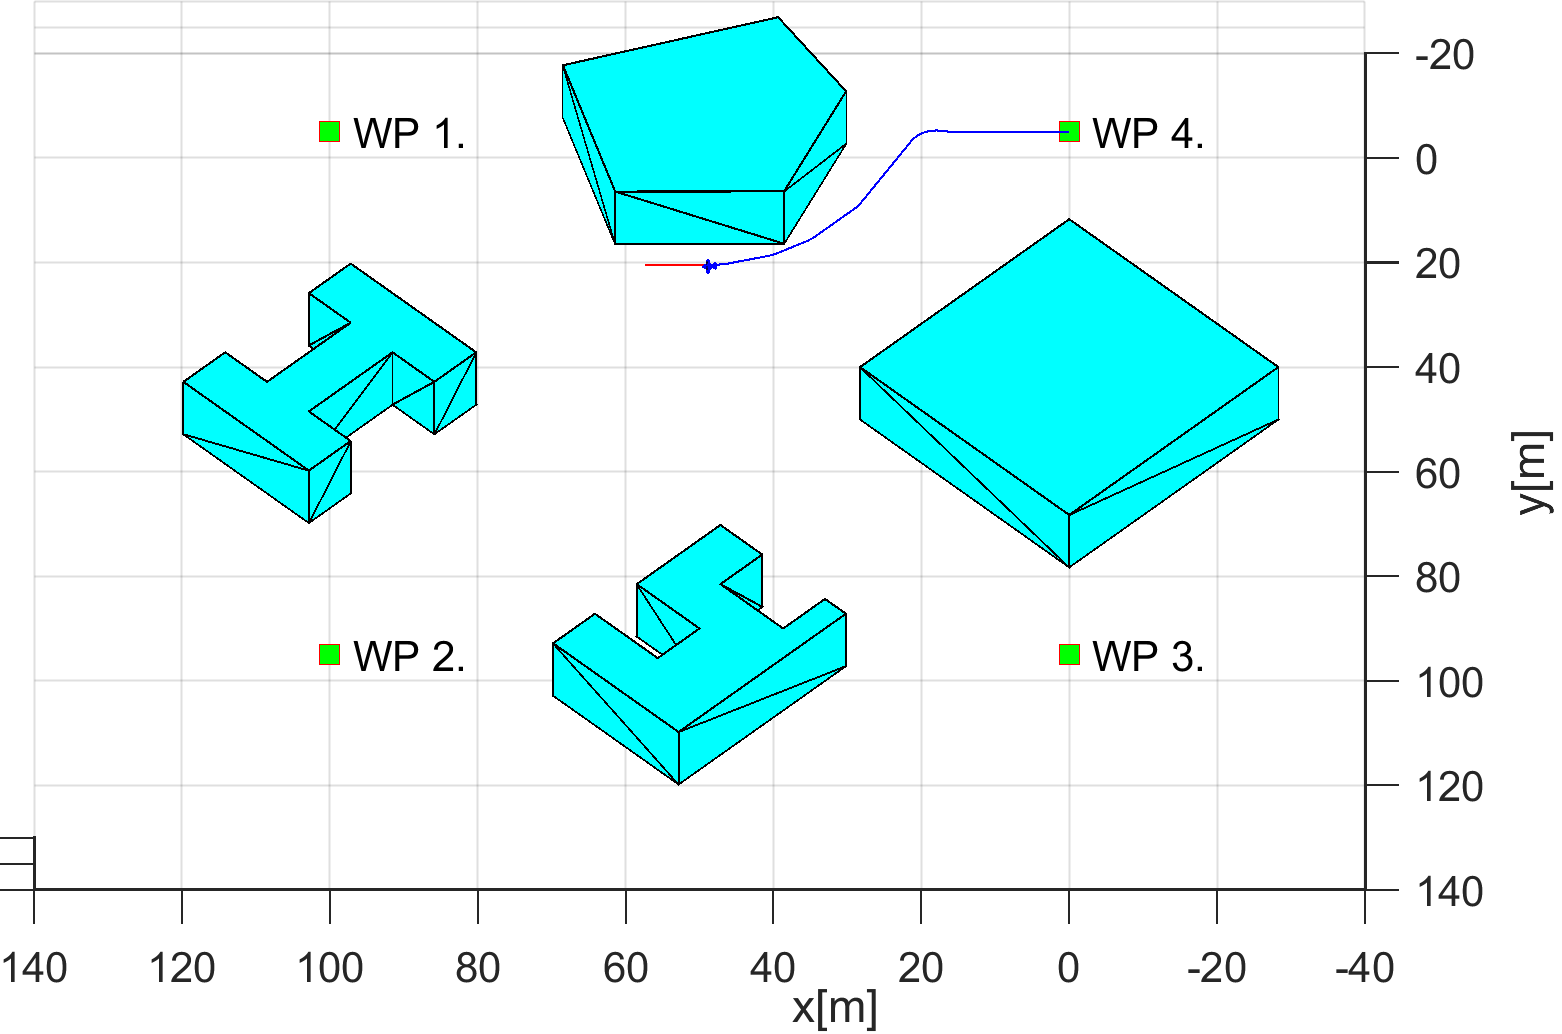
\includegraphics[width=0.9\linewidth]{\FIGDIR/NS001ConstraintsBuildingObstacle00061}
		\caption{$1^{st}$ building avoidance.}
		\label{fig:firstBuildingAvoidance}
	\end{subfigure}
	\begin{subfigure}{0.48\textwidth}
		\centering
		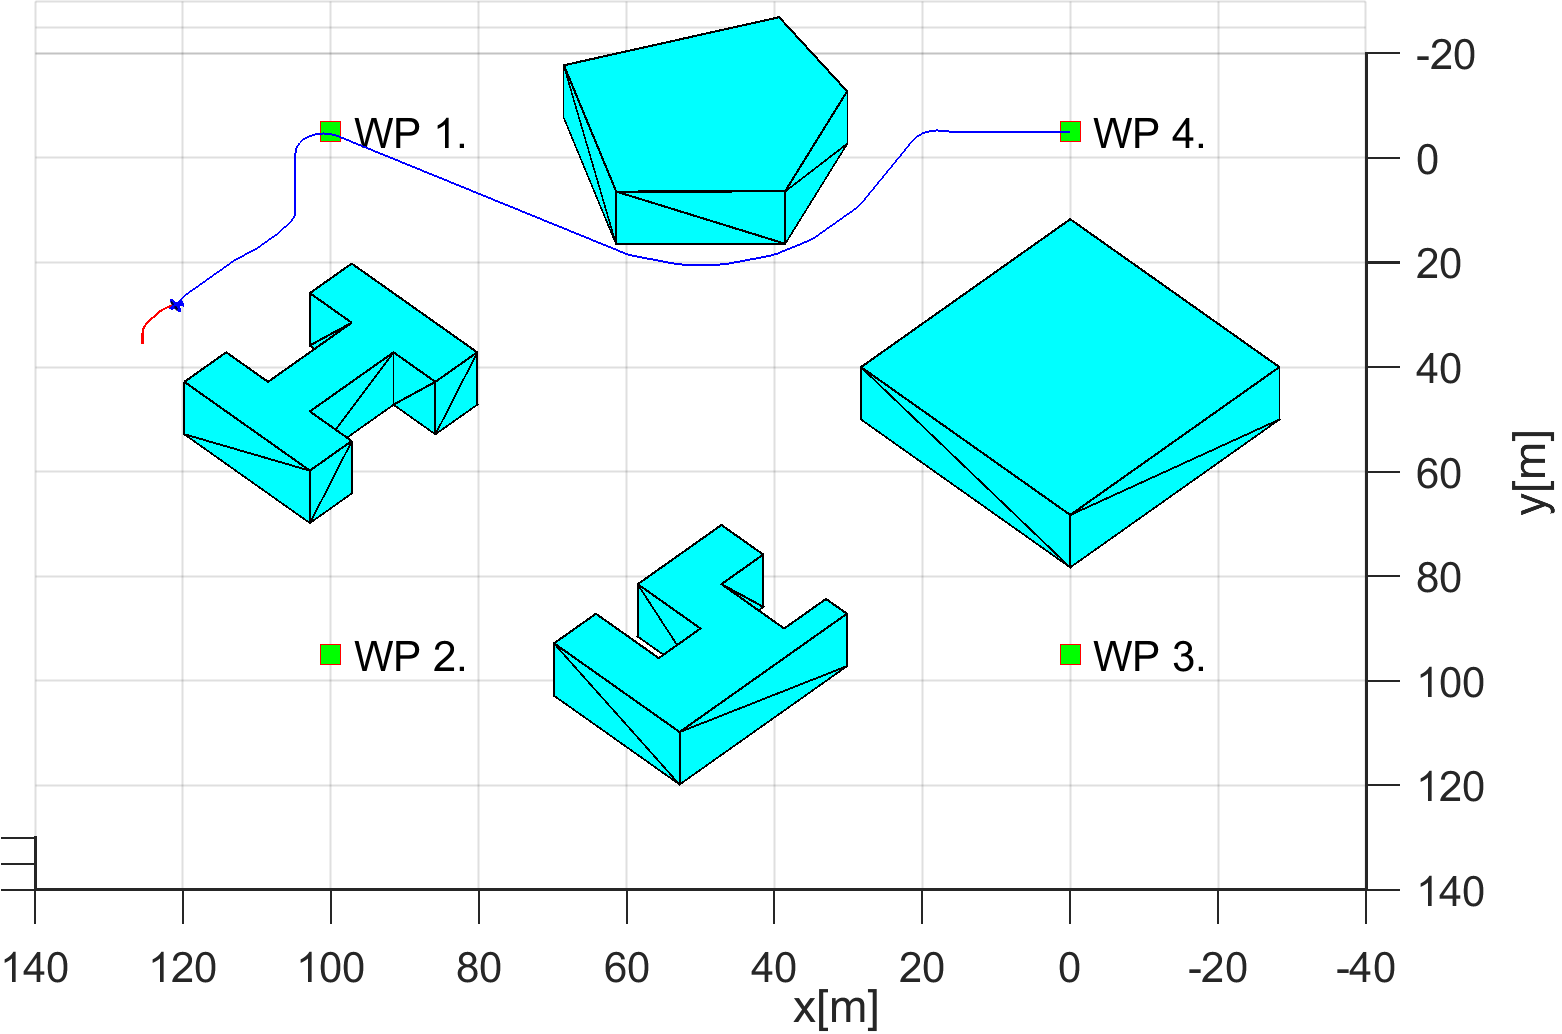
\includegraphics[width=0.9\linewidth]{\FIGDIR/NS002ConstraintsBuildingObstacles00161} 
		\caption{$1^{nd}$ building avoidance.}
		\label{fig:secondBuildingAvoidance}
	\end{subfigure}
	\\
	\begin{subfigure}{0.48\textwidth}
		\centering
		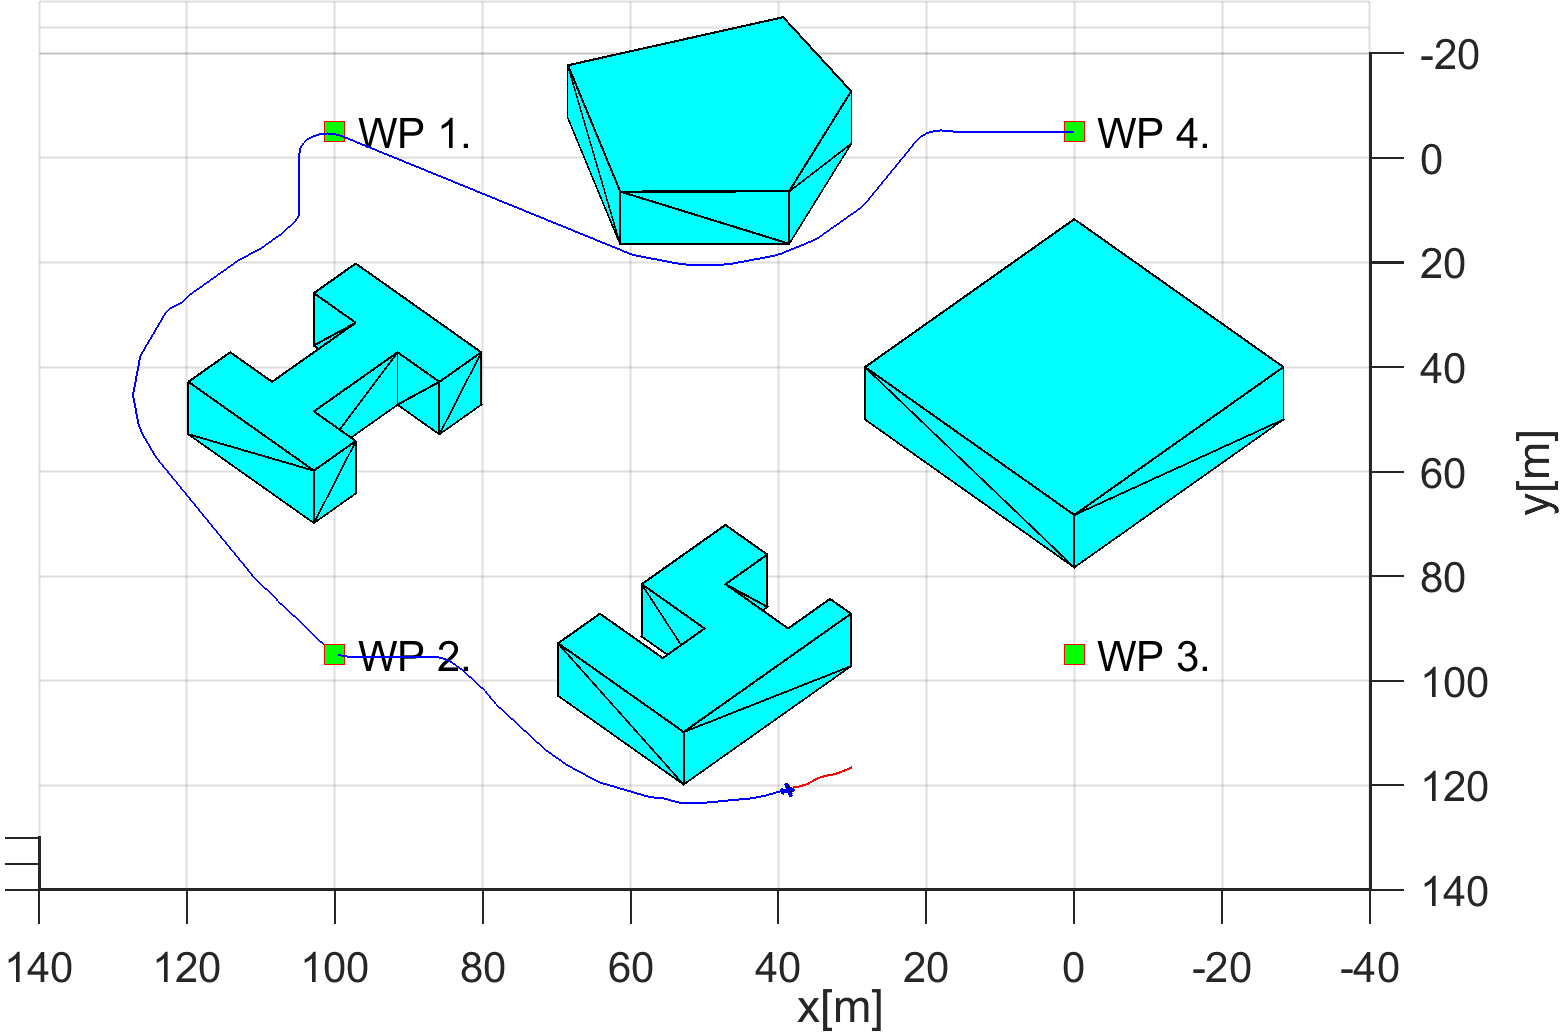
\includegraphics[width=0.9\linewidth]{\FIGDIR/NS003ConstraintsBuildingObstacles00311} 
		\caption{$3^{rd}$ building avoidance.}
		\label{fig:thirdBuidlingAvoidance}
	\end{subfigure}
	\begin{subfigure}{0.48\textwidth}
		\centering
		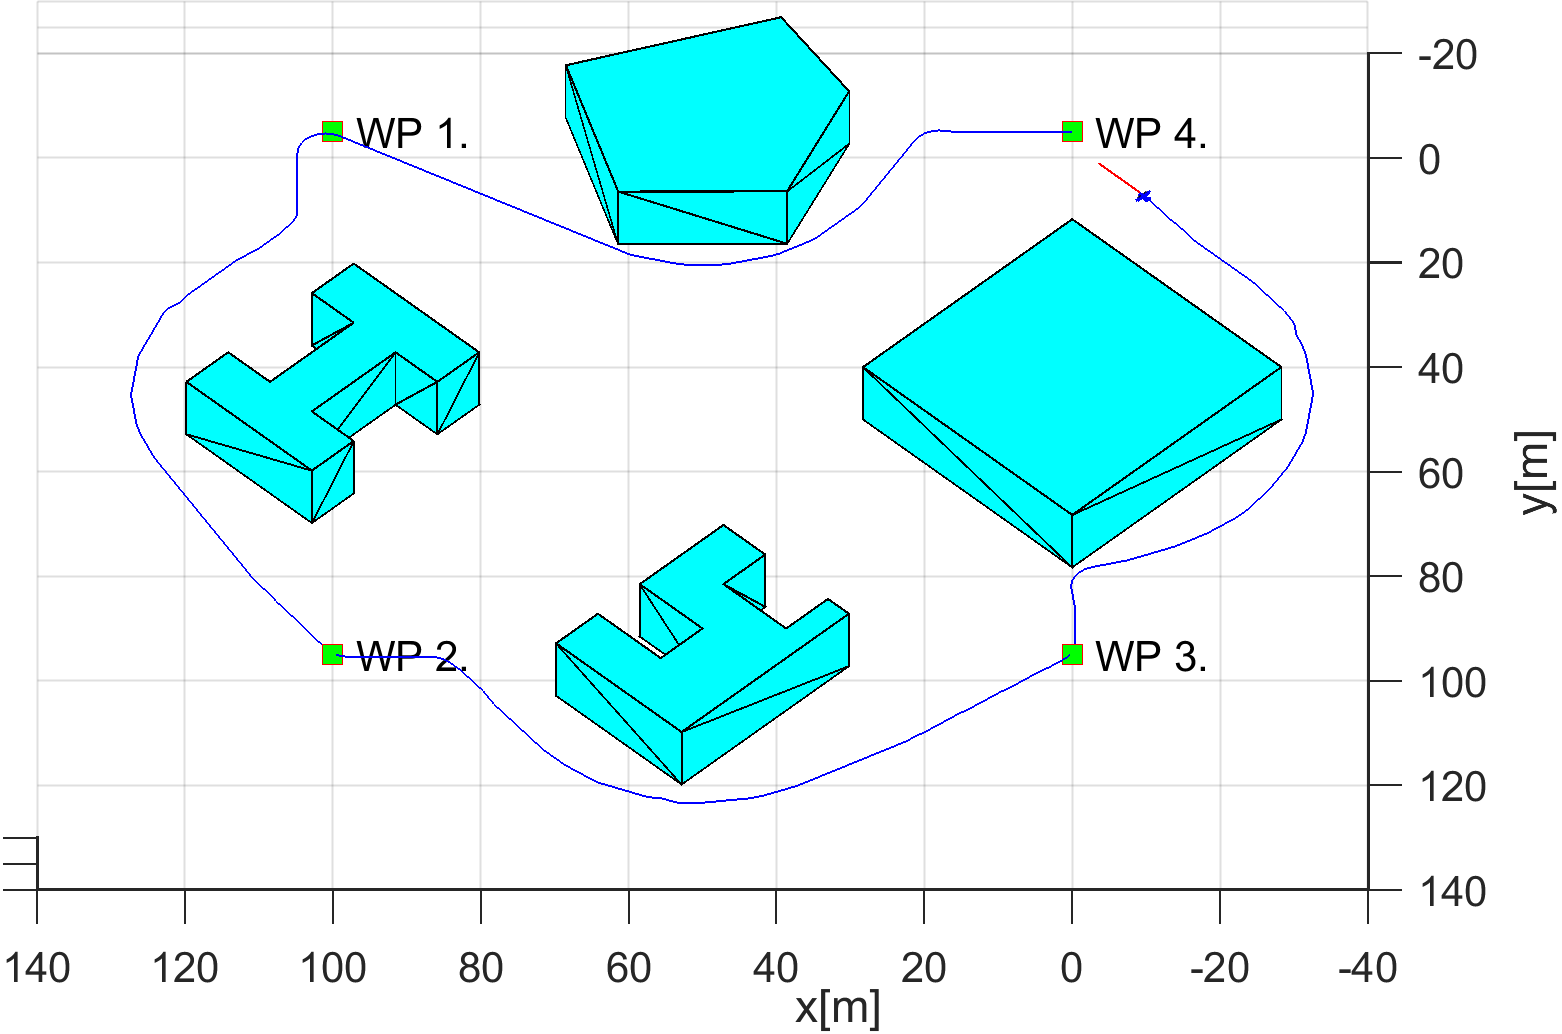
\includegraphics[width=0.9\linewidth]{\FIGDIR/NS004ConstraintsBuildingObstacles00470} 
		\caption{$4^{th}$ building avoidance.}
		\label{fig:fourthBuildingAvoidance}
	\end{subfigure}
	\caption{Test scenario for \emph{Building avoidance} (static ground obstacles). }
	\label{fig:testCaseBuildingAvoidanceSituation}
\end{figure}


\noindent\paragraph{Distance to Body/Safety Margin Evolution:} The distance of \emph{UAS} center to nearest obstacle (blue) does not broke a \emph{safety margin} (of closest obstacle (yellow)  nor \emph{body margin} of closest obstacle (red) as it can be seen in (fig. \ref{fig:testCaseBuildingAvoidancePerformance}). \emph{Acceptance condition} for \emph{algorithm mode switch} can be shown by UAS \emph{active avoidance of obstacles}.

\begin{note}
The \emph{body} and \emph{safety margins} are changing depending on \emph{UAS position and orientation}, is changing reflecting (tab. \ref{tab:obstacleSetBuildingAvoidance}) margins. 
\end{note}


\begin{figure}[H]
	\centering
	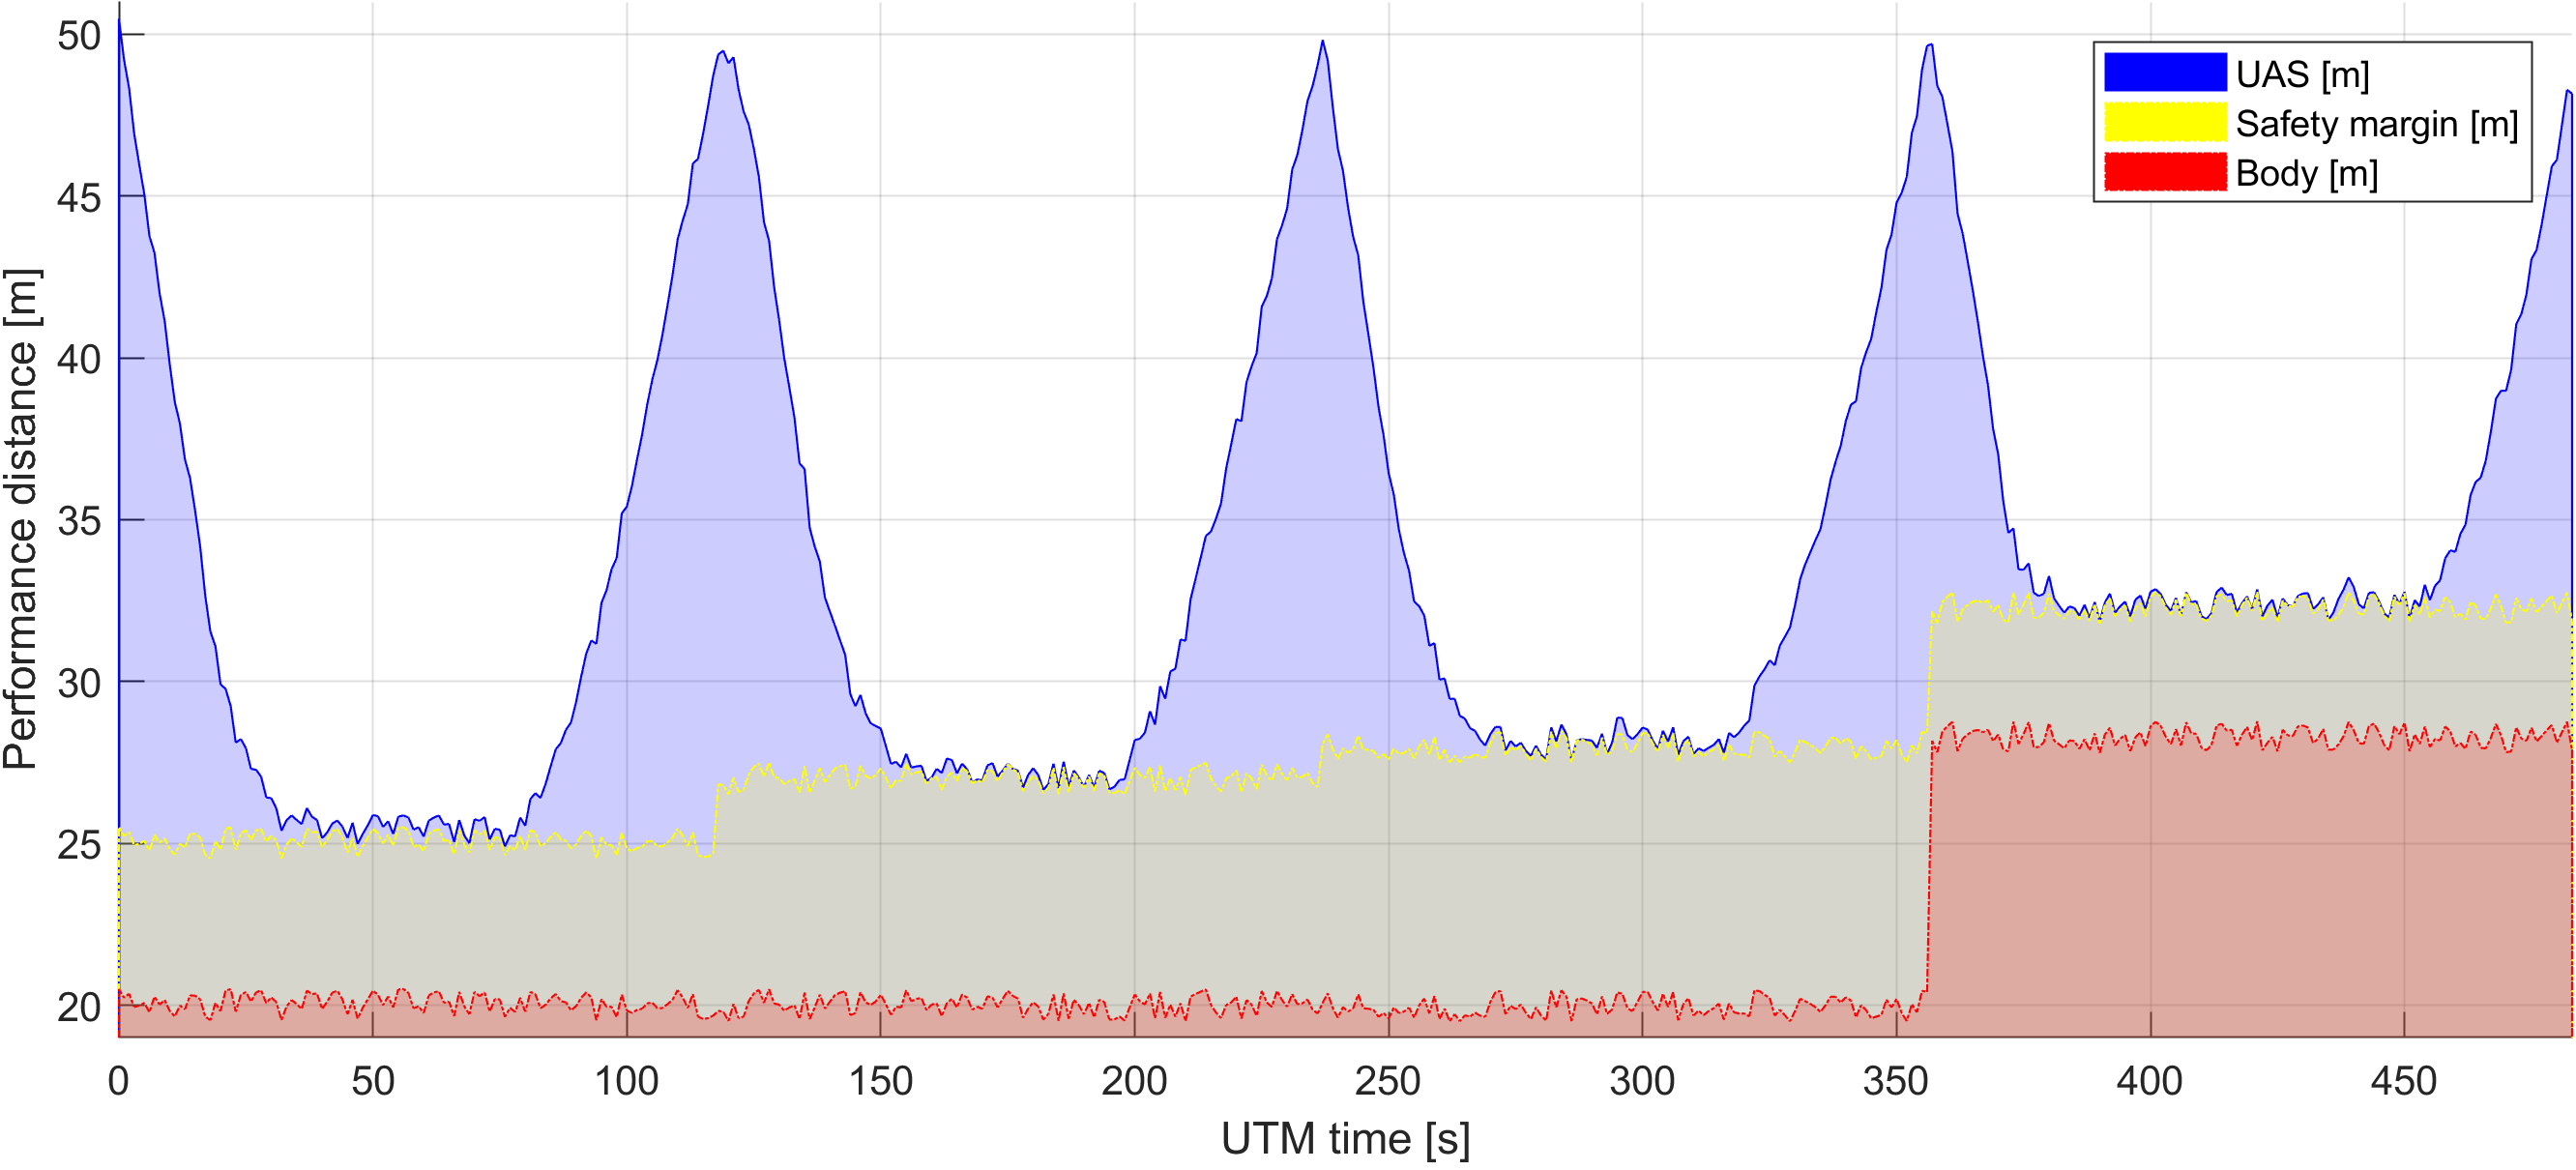
\includegraphics[width=0.8\linewidth]{\FIGDIR/NS005ConstraintsPolynomialBuildingObstaclesPerformance} 
	\caption{Distance to body/safety margin evolution for \emph{Building avoidance scenario}.}
	\label{fig:testCaseBuildingAvoidancePerformance}
\end{figure}


\noindent\paragraph{Distance to Body/Safety Margin Peaks:} Minimal distance to \emph{safety margin} is $0.69$ $m$. The \emph{minimal distance to obstacle body} is $4.69$ $m$ which is more than sufficient for tested UAS type. \emph{Safety margin acceptance criteria} have been achieved, because minimal distance is greater than zero. The minimal \emph{body margin distance} is $4.69$ $m$ for obstacle no. $4$ (tab. \ref{tab:obstacleSetBuildingAvoidance}).

\begin{table}[H]
	\centering
	\begin{tabular}{c|c||c}
	\multicolumn{2}{c||}{Parameter} & UAS 1 \\\hline\hline
	\multirow{2}{*}{Distance to Safety Margin} & min & 0.69  \\\cline{2-3}
											& max & 24.98 \\\hline
	\multirow{2}{*}{Distance to Body Margin}   & min & 4.69  \\\cline{2-3}
											& max & 29.98 
	\end{tabular}
	\caption{Distance to Body/Satety Margin Peaks for \emph{Building avoidance scenario}.}
	\label{tab:testCaseBuildingAvoidanceSafetyAndBodyMarginDistances}
\end{table}

\noindent\paragraph{Path Tracking Performance:} Reference path (green dashed line) is given as direct interconnection between waypoints (green numbered square).  The real trajectory (blue solid line) is split into its XYZ components. \emph{All mission waypoints} (fig. \ref{fig:testCaseBuildingAvoidancePathTracking}) have been reached in given order. There are some deviations on $X-Y$ horizontal axes, while the UAS was in the \emph{avoidance mode}.

\begin{figure}[H]
	\centering
	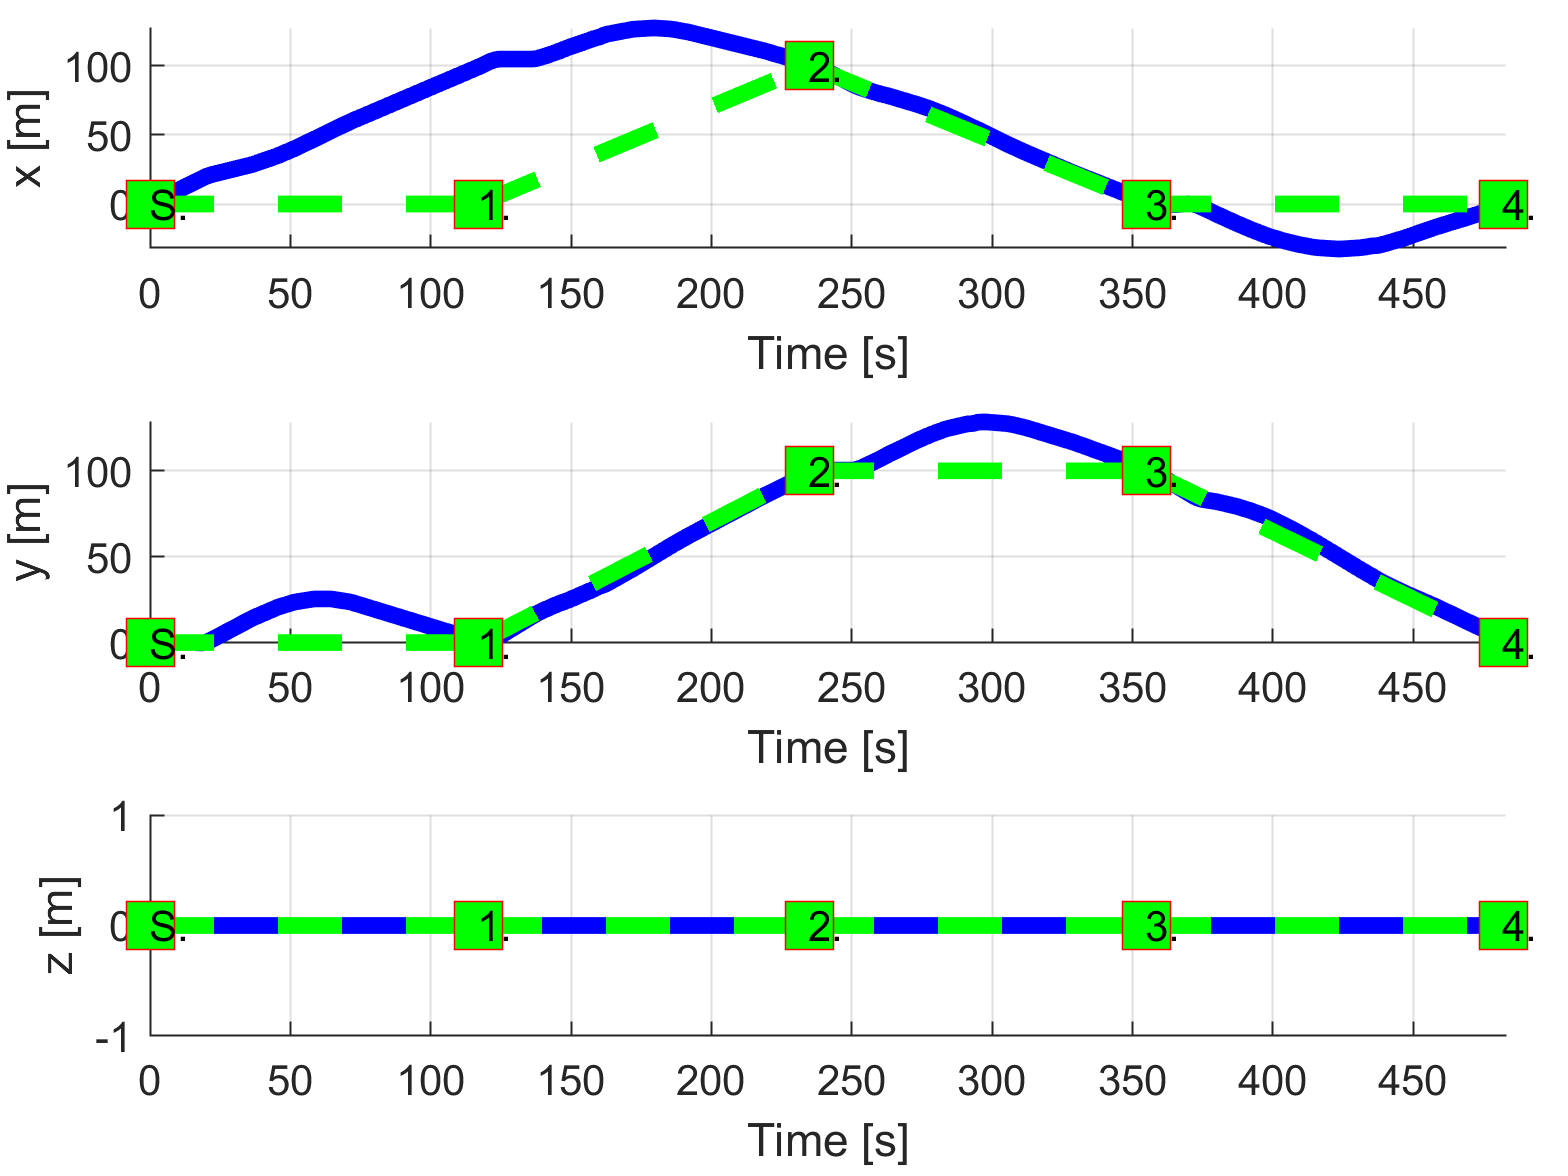
\includegraphics[width=0.55\linewidth]{\FIGDIR/NS006ConstraintsPolynomialBuildingPathFollowing} 
	\caption{\emph{Building avoidance} path tracking.}
	\label{fig:testCaseBuildingAvoidancePathTracking}
\end{figure}



\noindent\paragraph{Path Tracking Deviations:} Deviations (tab. \ref{tab:pathTrackingParametersForBuildingAvoidance}) from \emph{reference trajectory} are in expected ranges considering \emph{mission plan} (tab. \ref{tab:missionSetupForBuildingAvoidanceScenario}) and \emph{obstacle properties} (tab. \ref{tab:obstacleSetBuildingAvoidance}).
\begin{table}[H]
	\centering
	\begin{tabular}{c||c|c|c|c}
		\multirow{2}{*}{Param.} & \multicolumn{4}{c}{UAS 1} \\\cline{2-5}
						& $\mathscr{WP}_1$  & $\mathscr{WP_2}$  & $\mathscr{WP}_3$  & $\mathscr{WP}_4$  \\\hline\hline
		  $\max |x|$    & 104      & 86      & 5.34       & 32.52 \\\hline
		  $\max |y|$    & 25.39      & 6.59       & 28.2      & 4.55 \\\hline
		  $\max |z|$    & 0      & 0      &   0    & 0 \\\hline
		  $\max dist.$  & 107.05       & 86.2      & 28.7       & 32.84 \\
	\end{tabular}
	\caption{Path tracking for properties \emph{Building avoidance}.}
	\label{tab:pathTrackingParametersForBuildingAvoidance}
\end{table}

% 01-Building Avoidance Scenario:
\paragraph{Computation Load:} The \emph{computation load} for \emph{scenario} (fig.\ref{fig:buildingAvoidanceComputationTime}) shows used time (y-axis) over decision frame (x-axis).

There is slight increase in \emph{computation time} when UAS is in \emph{Emergency Avoidance Mode}.

\begin{figure}[H]
    \centering
    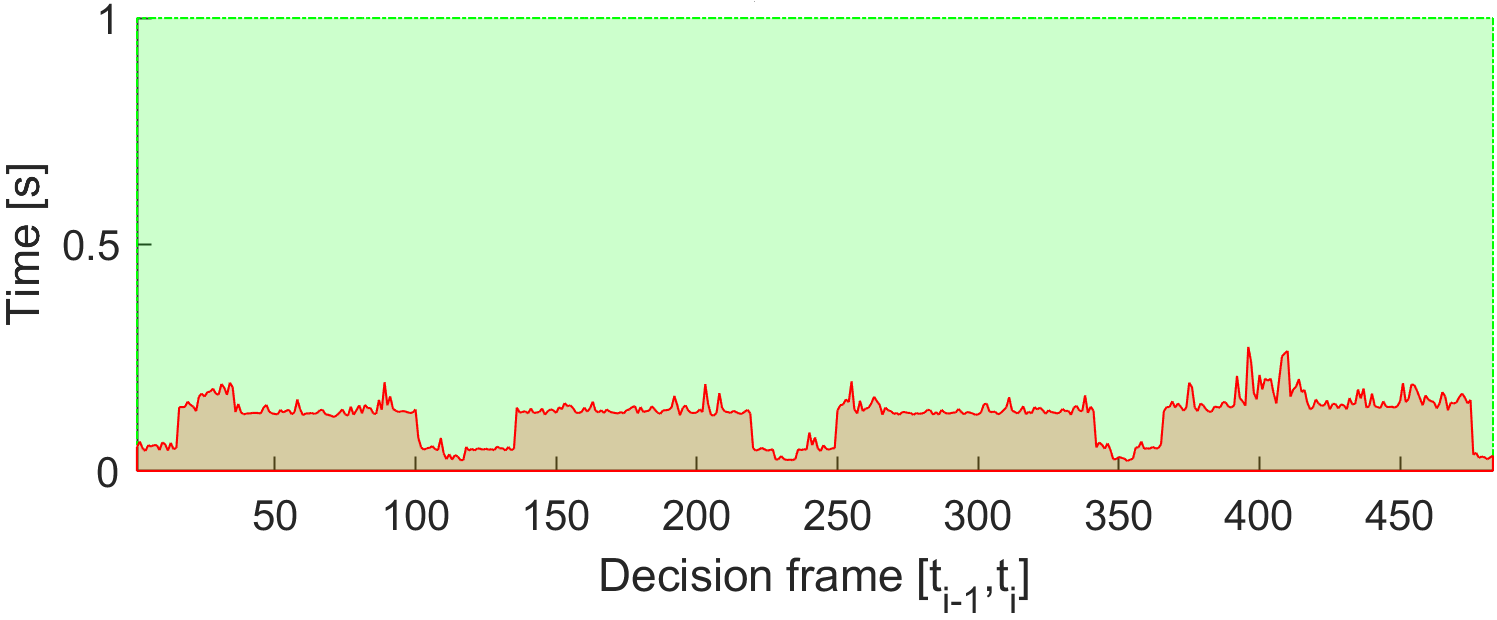
\includegraphics[width=0.65\linewidth]{\FIGDIR/NS092BuildingAvoidanceComputationTime} 
    \caption{Computation time for \emph{Building avoidance} scenario.}
    \label{fig:buildingAvoidanceComputationTime}
\end{figure}
  



    	\subsection{Slalom}\label{s:testSlalom}

\paragraph{Scenario:} The \emph{UAS} is flying the mission given by (tab. \ref{tab:missionSetupSlalomScenario}) in the \emph{open-space environment}. A Operational space is more clustered than in case of \emph{Building Avoidance} (sec. \ref{s:testBuildingAvoidance}). There map of notable \emph{buildings} with defined \emph{safety and body margins} imposing additional flight constraints. The \emph{UAS} is flying through partially known space with some charted obstacles. 

The \emph{goal waypoint} is hidden behind the sensors line of sight. There is multiple cost equivalent trajectories to reach the goal. 

\begin{table}[H]
    \centering
    \begin{tabular}{c|c||c}
        \multicolumn{2}{c||}{Position} & \multirow{2}{*}{$\mathscr{WP}_1$} \\\cline{1-2}
        $[x,y,z]$           & $[\theta,\varpi,\psi]$           & \\\hline\hline
        $[25,5,0]^T $        & $[0^\circ,0^\circ,90^\circ]^T$    & $[35,75,0]^T$        \\ 
    \end{tabular}
    \caption{Mission setup for \emph{Slalom} scenario.}
    \label{tab:missionSetupSlalomScenario}
\end{table}

\paragraph{Obstacle set:} Obstacles are discovered during a flight by \emph{UAS LiDAR Sensor}. The set of obstacles is defined in (tab. \ref{tab:obstacleSetSlalom}) Some obstacles does not have \emph{Line of Sight} during a flight, which causes additional constraints during \emph{avoidance trajectory selection} process.

\begin{table}[H]
    \centering
    \begin{tabular}{c|c|c|c|c|c}
        \multicolumn{2}{c|}{Obstacle} & \multicolumn{3}{c|}{Body Margin} & \multirow{2}{*}{Safety Margin}\\\cline{1-5}
        position & type & min. & max. & avg. &   \\\hline\hline
        multiple (4) & hospital & $[0.5,1]$ & $[2.2,3.1]$ & $[1.5,3]$  & $[1,3]$ \\\hline 
        multiple (7) & unusual  & $[0.3,1]$ & $[2.3,3.5$] & $[2,3]$  & $[1,4]$ \\\hline
        multiple (3) & square   & $[3,4]$   & $[4,5]$     & $[4,5]$ & $[1,4]$   \\
     \end{tabular}
    \caption{\emph{Obstacle set} for \emph{Slalom} scenario.}
    \label{tab:obstacleSetSlalom}
\end{table}

\paragraph{Main goal:} Show \emph{static obstacle avoidance} in \emph{clustered environment} with \emph{shorter decision frames} due the obstacle density. Show \emph{hidden waypoint navigation capability} and Behind Line of Sight impact on decision making. 

\paragraph{Acceptance Criteria} are given as follow: 
\begin{enumerate}
    \item \emph{Hidden waypoint reach} - the UAS will safely reach \emph{goal waypoint}.
    \item \emph{Minimal safety margin distance} $\ge$ 0.
    \item \emph{Hindered space} is accounted into decision making (BLOS impact).
\end{enumerate}

\paragraph{Testing setup:}  The \emph{standard test setup} defined in (tab.  \ref{tab:testMovementOrientations}. \ref{tab:testUASBasicParameters}. \ref{tab:testNavigationGridBasic}. \ref{tab:testAvoidanceGridBasic}. \ref{tab:testUASColoring}) is used with following parameter override:

\begin{enumerate}
    \item \emph{Avoidance grid - type} - \emph{ACAS-like} with enabled \emph{Horizontal maneuvers}
\end{enumerate}

\begin{note}
The \emph{vertical separation} was disabled, because \emph{UAS} will just increase its altitude to reach \emph{goal waypoint}.
\end{note}

\paragraph{Simulation run:} Notable moments from this \emph{simulation run} (fig. \ref{fig:testCaseSlalomwithHiddenWaypoint}) are following:

\begin{enumerate}
    \item \emph{Open space obstacle} (fig. \ref{fig:slalomOpenSpaceObstacle}) - avoidance of open space obstacle, while tracking \emph{hidden waypoint}. This is standard navigation procedure, the middle building in front of \emph{goal waypoint} is hidden by building in front of UAS.
        
    \item \emph{Hidden waypoint navigation} is shown in three stages start (fig. \ref{fig:slalomHiddenWaypointStart}), middle (fig. \ref{fig:slalomHiddenWaypointMiddle}), and end phase (fig. \ref{fig:slalomHiddenWaypointEnd}).The \emph{hidden goal waypoint} has been reached and first acceptance criteria was fullfilled.  The \emph{Decision points} of navigational loop are placed in very high density around this area. The avoided building had following traps which were avoided:
    
    \begin{enumerate}[a.]
        \item Trap (fig. \ref{fig:slalomHiddenWaypointStart}) on the left side of \emph{UAS} was avoided, because there was no turning point inside of space.
    
        \item Trap (fig. \ref{fig:slalomHiddenWaypointMiddle}) on the left side of UAS was avoided, because it was not wide enough to be considered as trajectory space.
    \end{enumerate}
\end{enumerate}


\begin{figure}[H]
    \centering
    \begin{subfigure}{0.48\textwidth}
    	\centering
        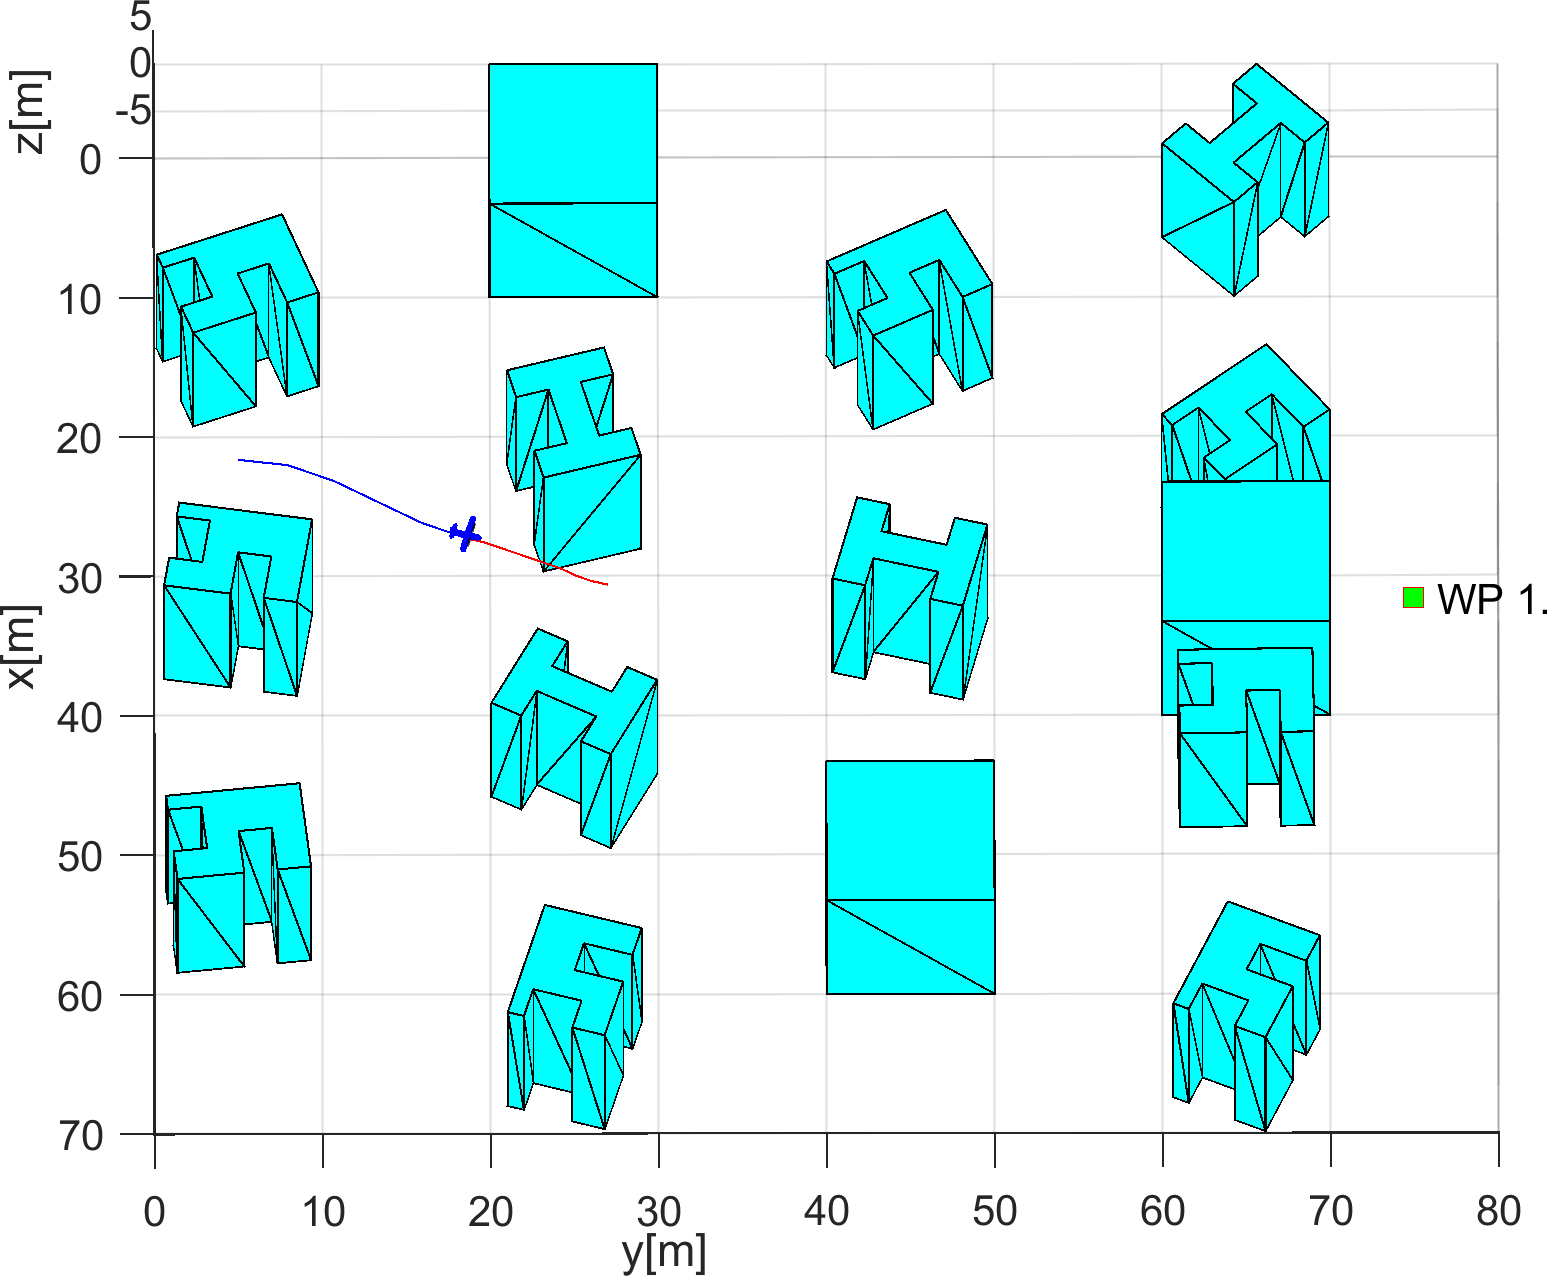
\includegraphics[width=0.9\linewidth]{\FIGDIR/NS007ConstraintsPolynomialSlalom-00015}
        \caption{Open space obstacle.}
        \label{fig:slalomOpenSpaceObstacle}
    \end{subfigure}
    \begin{subfigure}{0.48\textwidth}
    	\centering
        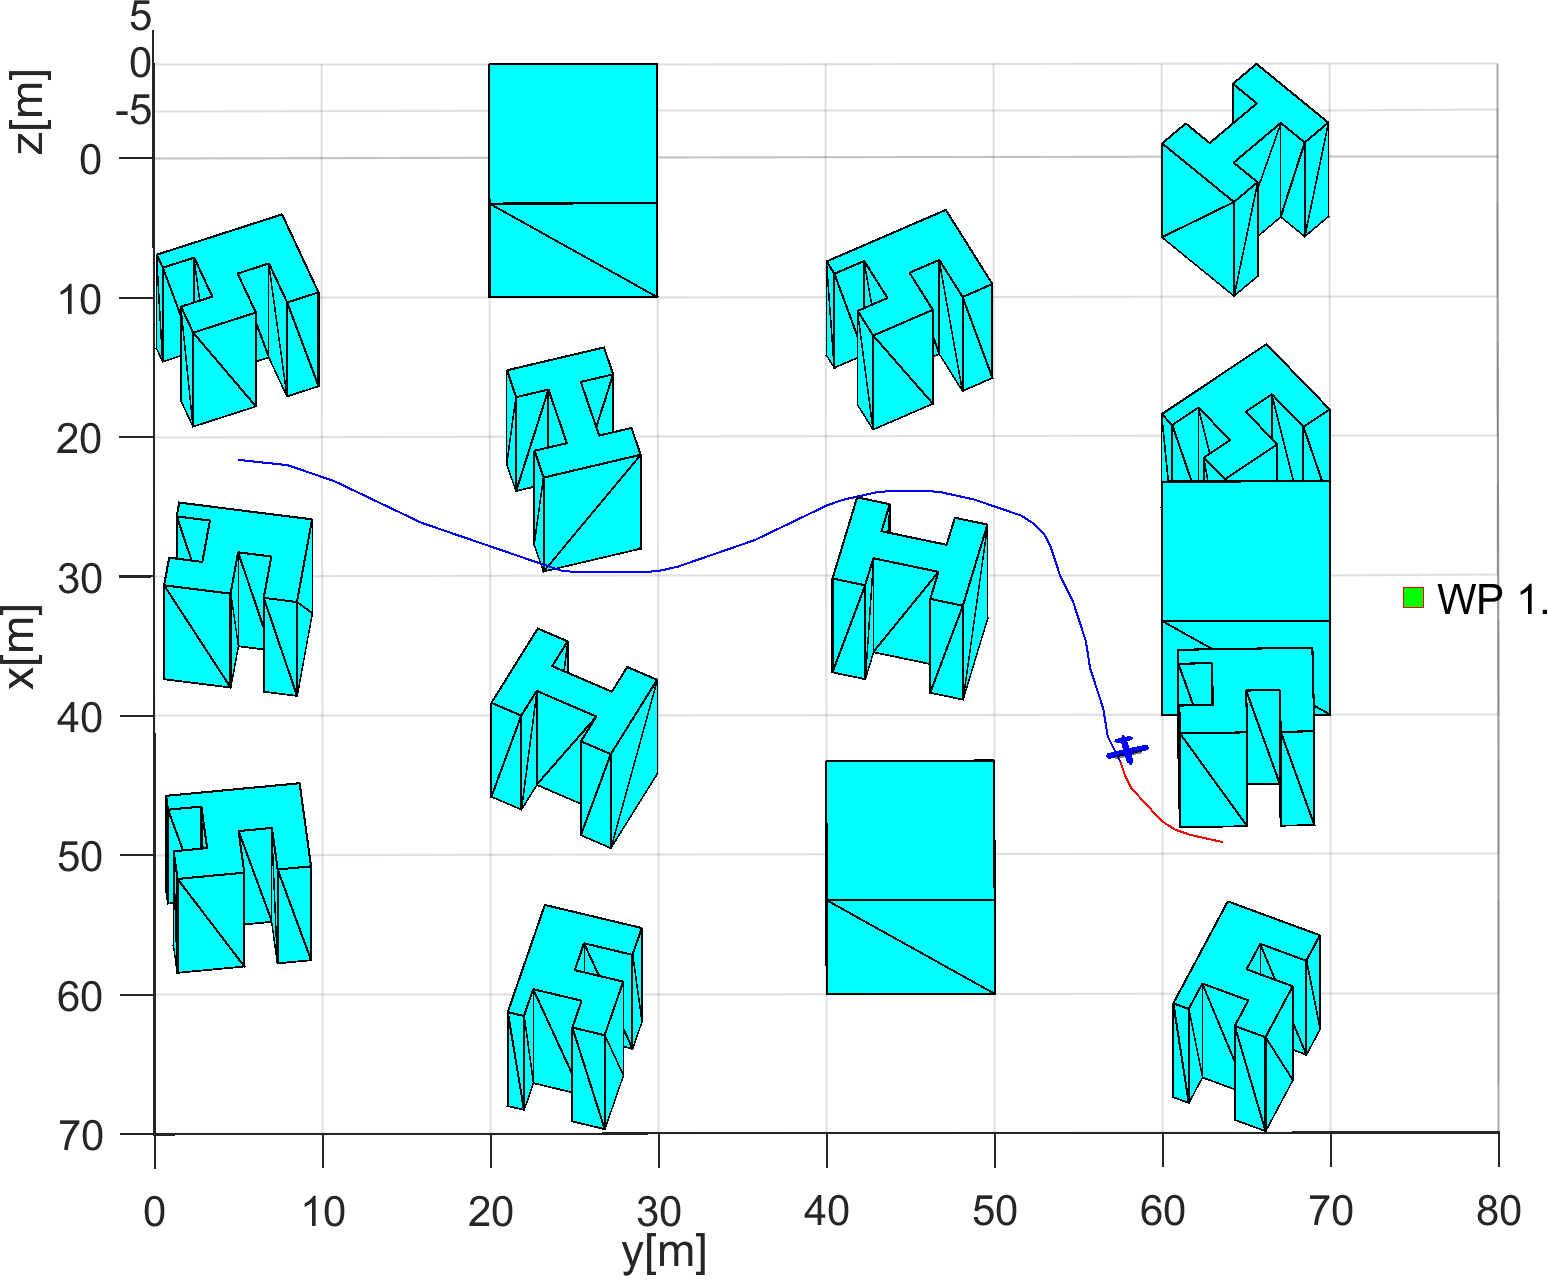
\includegraphics[width=0.9\linewidth]{\FIGDIR/NS008ConstraintsPolynomialSlalom-00069} 
        \caption{Hidden waypoint start.}
        \label{fig:slalomHiddenWaypointStart}
    \end{subfigure}
    \\
    \begin{subfigure}{0.48\textwidth}
	    \centering
        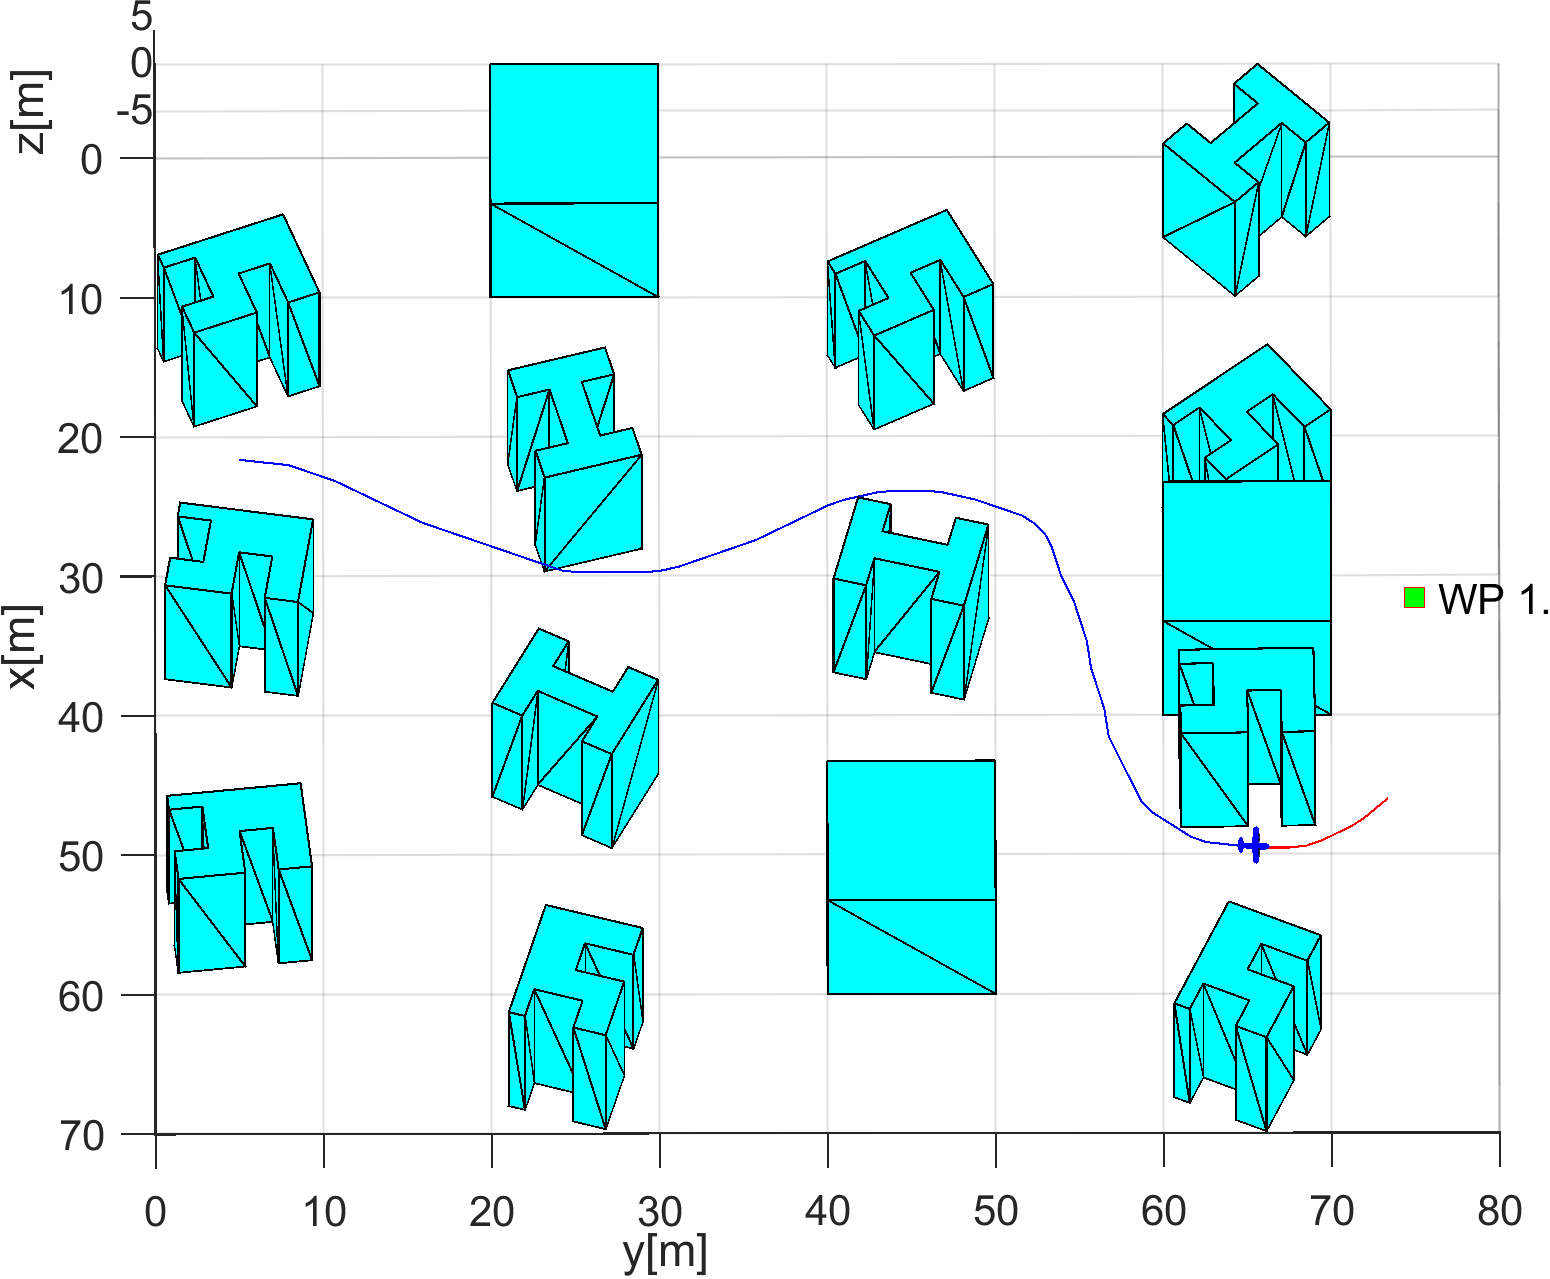
\includegraphics[width=0.9\linewidth]{\FIGDIR/NS009ConstraintsPolynomialSlalom00080} 
        \caption{Hidden waypoint middle.}
        \label{fig:slalomHiddenWaypointMiddle}
    \end{subfigure}
    \begin{subfigure}{0.48\textwidth}
    	\centering
        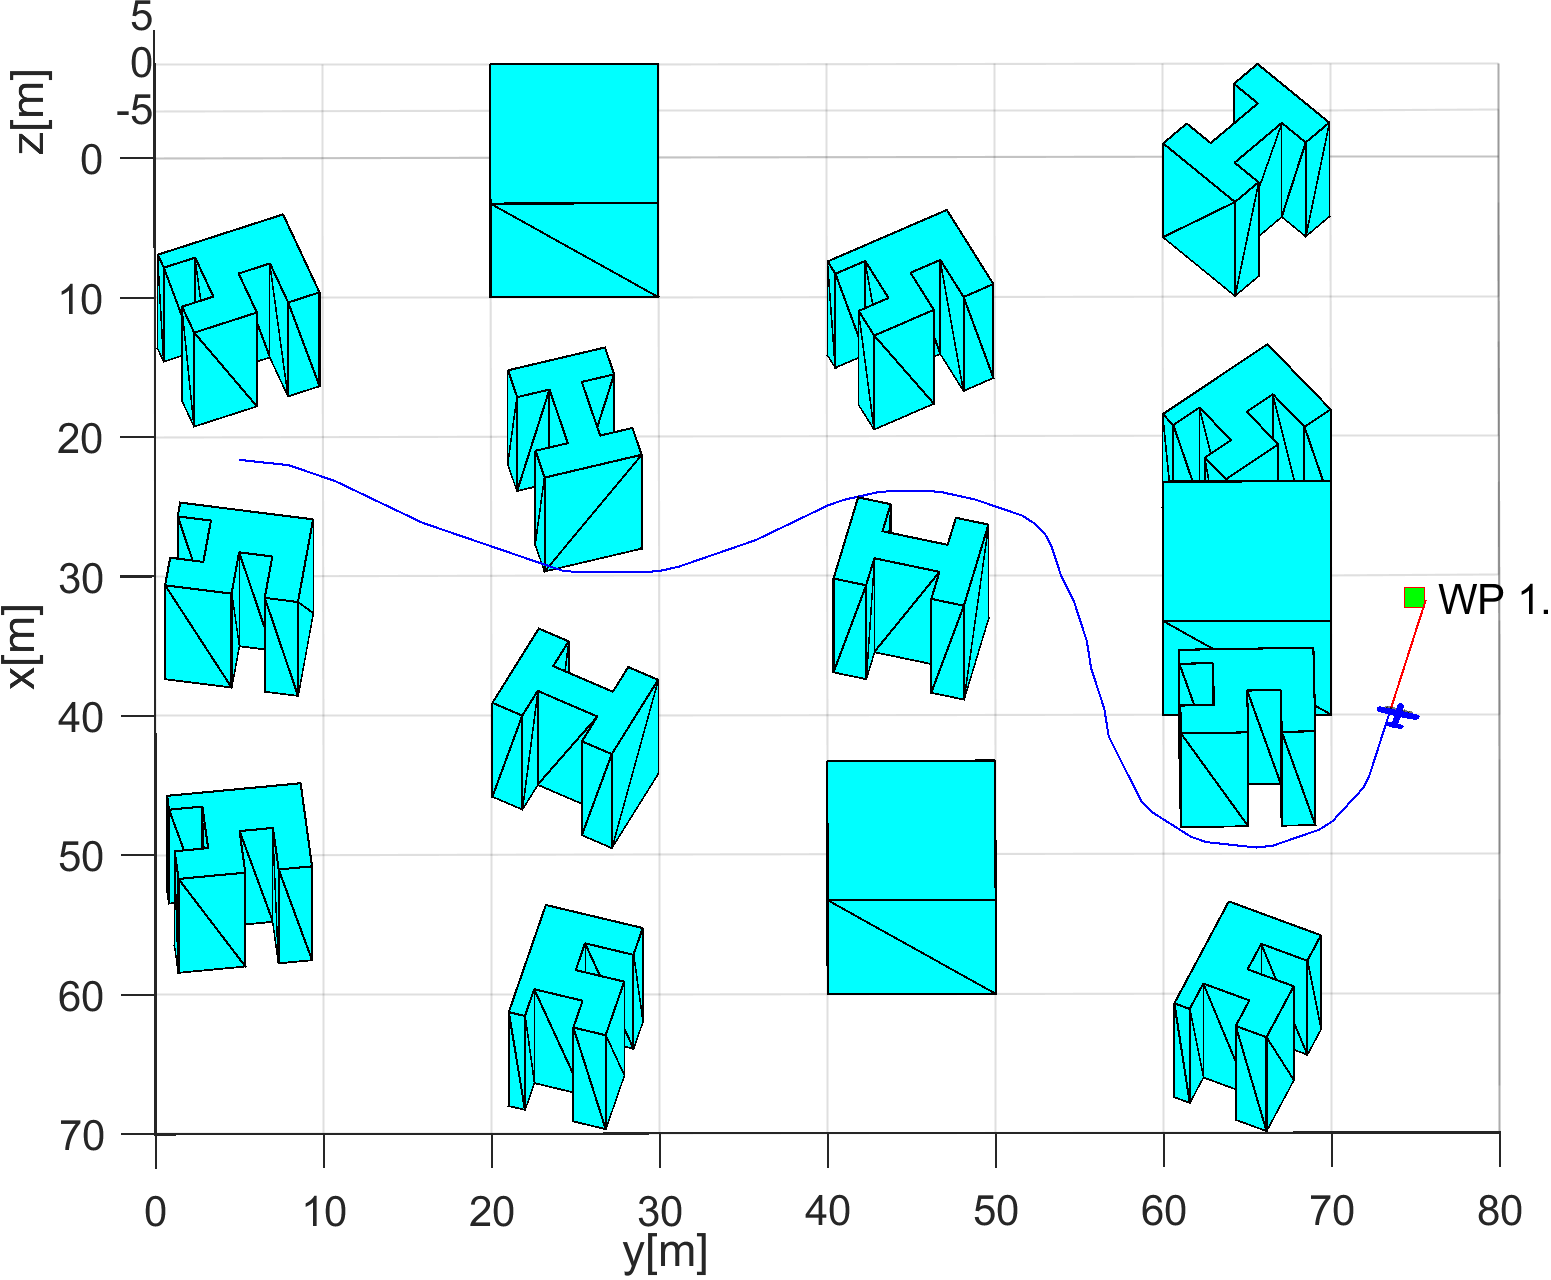
\includegraphics[width=0.9\linewidth]{\FIGDIR/NS010ConstraintsPolynomialSlalom00094} 
        \caption{Hidden waypoint end.}
        \label{fig:slalomHiddenWaypointEnd}
    \end{subfigure}
    \caption{Test scenario for \emph{Slalom} with \emph{hidden waypoint}. }
    \label{fig:testCaseSlalomwithHiddenWaypoint}
\end{figure}


\paragraph{Distance to Safety Margin Evolution:} The \emph{UAS} (blue fill) does not break a \emph{safety margin} (yellow fill) nor \emph{body margin} (red fill) as you can seen in (fig. \ref{fig:testCaseSlalomAvoidancePerformance}). Hindered space is accounted into decision making, because the distance to closest obstacle will never breach \emph{safety margin} (yellow fill). If it was not, the UAS will break \emph{safety} or \emph{body} margin. 

\emph{Body} and \emph{Safety margin} are changing values depending on the \emph{nearest obstacle} and \emph{mutual position of obstacle and UAS}. The ranges of \emph{body} and \emph{safety margins} are reflected in (tab. \ref{tab:obstacleSetSlalom}). 

\begin{figure}[H]
    \centering
    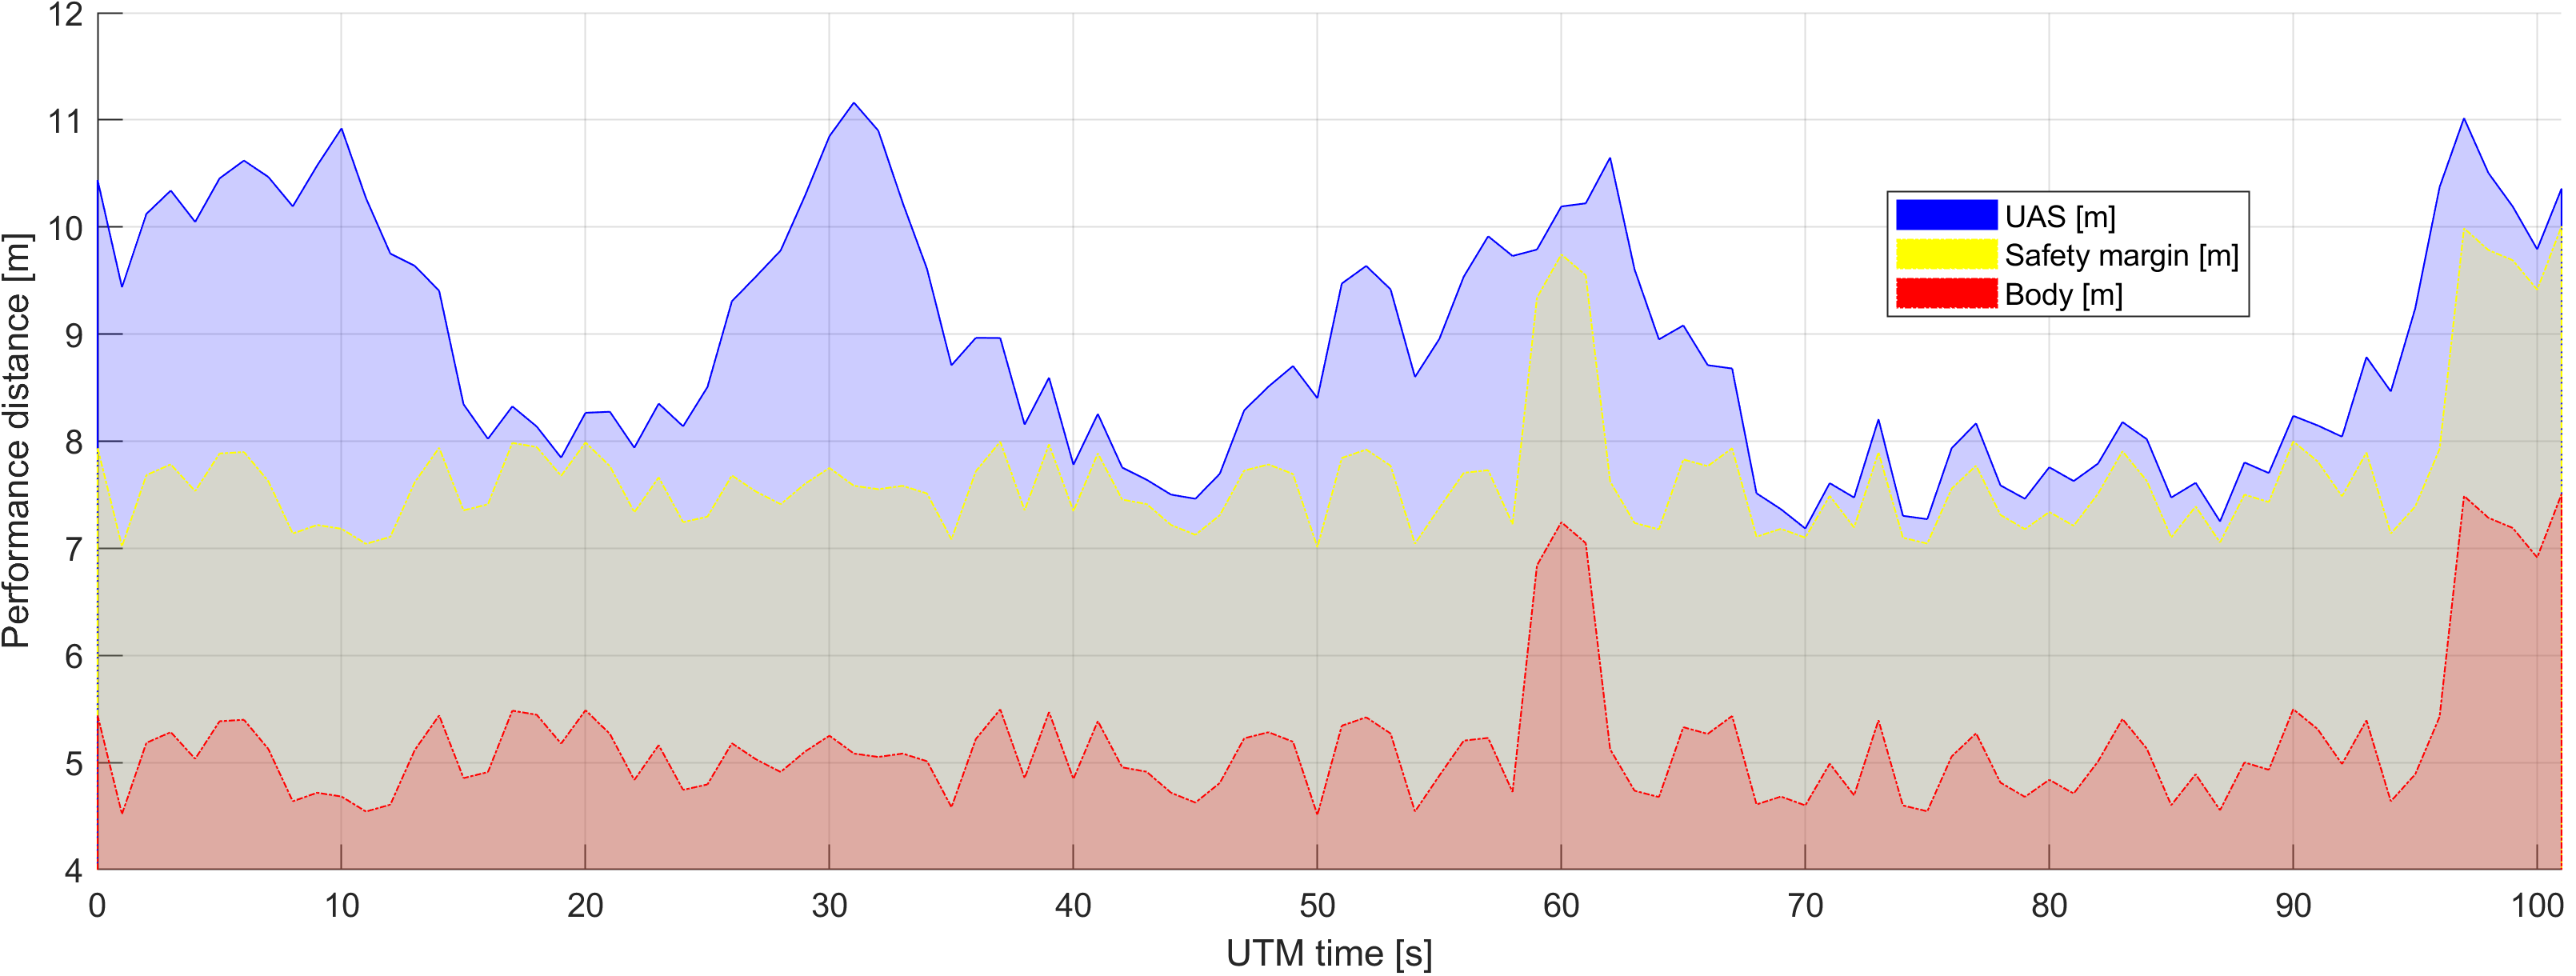
\includegraphics[width=0.8\linewidth]{\FIGDIR/NS011ConstraintsPolynomialSlalomPerformance} 
    \caption{Distance to Safety Margin Evolution for \emph{Slalom scenario}.}
    \label{fig:testCaseSlalomAvoidancePerformance}
\end{figure}

\paragraph{Distance to Safety Margin Peaks:} The boundary of \emph{safety} and  \emph{body} margin is given in (tab. \ref{tab:testCaseSlalomSafetyAndBodyMarginDistances}). The minimal distance of \emph{UAS border}(blue line) to \emph{safety margin boundary} (yellow line fig. \ref{fig:testCaseSlalomAvoidancePerformance}) is $0.0856$ $m$ which can be considered as marginal $0$. The minimal \emph{body margin} distance is $2.5856$ $m$ which is reflects \emph{safety margin} $2.5$ $m$ at that moment. The condition $safety Margin Distance \ge 0$ holds.
    
    
The difference between minimal and maximal \emph{safety margin distance} is $\sim 3$ $m$ which indicates that mission environment is  tightly packed with obstacles.

\begin{table}[H]
    \centering
    \begin{tabular}{c|c||c}
    \multicolumn{2}{c||}{Parameter} & UAS 1 \\\hline\hline
    \multirow{2}{*}{safety margin distance} & min & 0.0856\\\cline{2-3}
                                            & max & 3.7391 \\\hline
    \multirow{2}{*}{body margin distance}   & min & 2.5856  \\\cline{2-3}
                                            & max & 6.2391 
    \end{tabular}
    \caption{\emph{Slalom} safety and body margin distances.}
    \label{tab:testCaseSlalomSafetyAndBodyMarginDistances}
\end{table}


\paragraph{Path tracking performance:} Path tracking is given in (fig. \ref{fig:testCaseSlalomPathTracking}). The line between Starting position (green square, marked S) and  goal waypoint (green square marked 1) is reference trajectory (green dashed line). The flown trajectory (blue solid line) is showing evolution over mission time (Time [s]) in global coordinate frame split into three axes (x[m], y[m], z[m]). The UAS was all time in \emph{Emergency Avoidance Mode} due the vicinity of dangerous obstacles. 

The \emph{UAS} reached final navigation waypoint, which fulfills acceptance criteria. The UAS has taken a significant detour (x[m] evolution) due to hidden \emph{waypoint}. 

The test has been run multiple times to check if \emph{Right-Up} preference for avoidance is always selected. \emph{Small noise} (0.5-1m) was added to obstacle positions. The algorithm always chose similar deterministic path. The higher noise levels were not possible due the obstacle original size (tab. \ref{tab:obstacleSetSlalom}).

\begin{figure}[H]
    \centering
    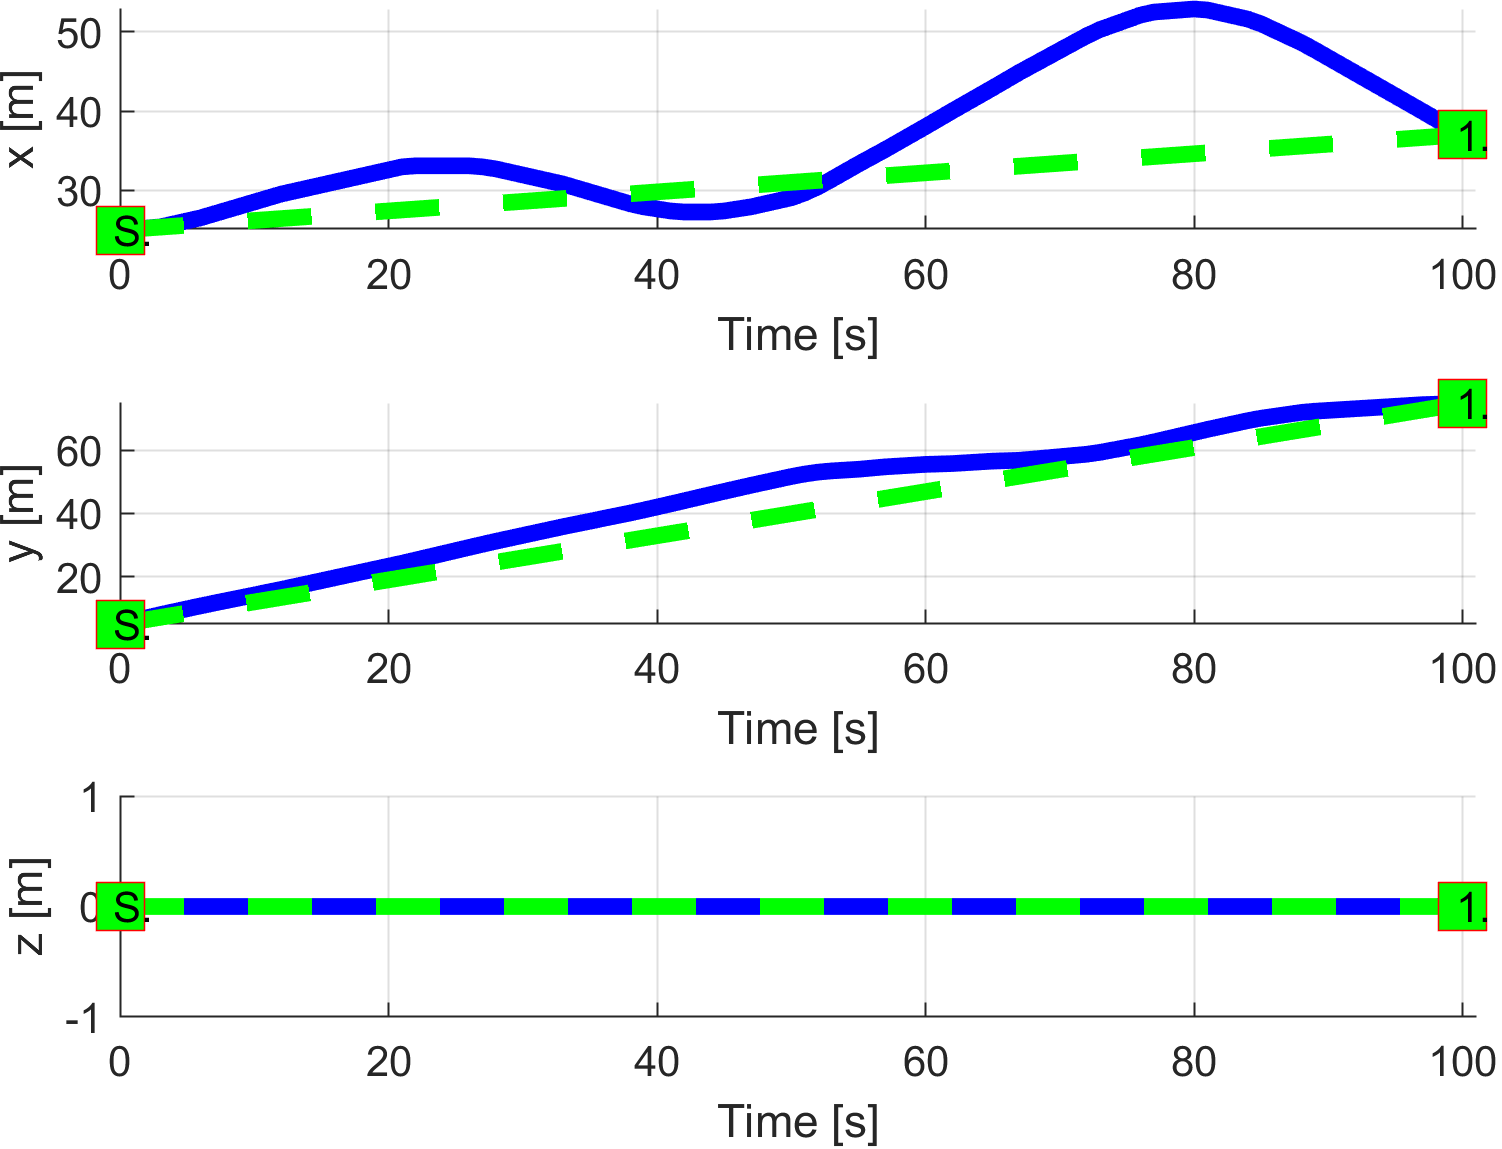
\includegraphics[width=0.55\linewidth]{\FIGDIR/NS012ConstraintsPolynomialSlalomPathFollowing} 
    \caption{\emph{Slalom} path tracking.}
    \label{fig:testCaseSlalomPathTracking}
\end{figure}


\paragraph{Path Tracking Deviations:} Deviations given in (tab. \ref{tab:pathTrackingParametersForSlalomAvoidance}) from \emph{reference trajectory} (fig. \ref{fig:testCaseSlalomPathTracking}) are in expected ranges considering \emph{mission plan} (tab. \ref{tab:missionSetupSlalomScenario}) and \emph{obstacle properties} (\ref{tab:obstacleSetSlalom}).

\begin{table}[H]
    \centering
    \begin{tabular}{c||c}
        \multirow{2}{*}{Param.} & UAS 1\\\cline{2-2}
                        & $\mathscr{WP}_1$  \\\hline\hline
          $\max |x|$    & 17.90      \\\hline
          $\max |y|$    & 12.41    \\\hline
          $\max |z|$    & 0        \\\hline
          $\max dist.$  & 20.06   \\
    \end{tabular}
    \caption{Path tracking properties for \emph{Slalom} scenario.}
    \label{tab:pathTrackingParametersForSlalomAvoidance}
\end{table}





    	\subsection{Maze}\label{s:testMaze}

\paragraph{Scenario:} The UAS is flying a mission given by (tab. \ref{tab:missionSetupMazeScenario}) in \emph{closed space} constrained by ground from bottom, airspace constraint from top and building from sides. The maneuverable space is \emph{maze-like} with  \emph{hidden goal waypoint}.

There exists a \emph{Obstacle map} with defined \emph{safety} and \emph{body margins}. \emph{Reference trajectories} (direct interconnection of initial position and \emph{goal waypoint}) is going trough \emph{partially known space} with some charted obstacles.

\begin{table}[H]
    \centering
    \begin{tabular}{c|c||c}
        \multicolumn{2}{c||}{Position} & \multirow{2}{*}{$\mathscr{WP}_1$} \\\cline{1-2}
        $[x,y,z]$           & $[\theta,\varpi,\psi]$           & \\\hline\hline
        $[15,15,0]^T $        & $[0^\circ,0^\circ,0^\circ]^T$    & $[15,75,0]^T$        \\ 
    \end{tabular}
    \caption{Mission setup for \emph{Maze} scenario.}
    \label{tab:missionSetupMazeScenario}
\end{table}

\paragraph{Obstacle set:} \emph{Obstacles} are discovered during a flight by \emph{UAS LiDAR} sensor. The \emph{Obstacle set} is defined in (tab. \ref{tab:obstacleSetMaze}). the obstacles are placed in \emph{virtual grid} with \emph{cell size} $10 \times 10 m$. There are following obstacles:

\begin{enumerate}
    \item $5\times$  \emph{Hospital building} - H-shaped, with two open traps, with minimal body margin in range $0.5 - 1m$, with maximal body margin in range $2.2 - 3.1 m$ and variable \emph{safety margin} in range $1-3 m$.
    
    \item $12\times$ \emph{Unusual trap building} - square shaped building with two traps on neighbouring side, with minimal body margin in range $0.3 - 1m$, with maximal body margin in range $2.3 - 3.5 m$ and variable \emph{safety margin} in range $1-4 m$.
    
    \item $6\times$  \emph{Square building} - square shaped building with minimal body margin in range $3-4 m$, with maximal body margin in range $4-5 m$ and variable \emph{safety margin} in range $1-4m$.
    
    \item $7\times$  \emph{U-shaped Trap} - thin walled U shaped trap designed to catch incoming flying objects, with minimal body margin in range $2-4m$, maximal body margin in range $3-5 m$ and various \emph{safety margin} in range $1-2 m$.
\end{enumerate}

The purpose of these \emph{Obstacles} except \emph{Square building} type is to create false positive path diversions. These diversions are designed to take \emph{UAS} into unsolvable situation. \emph{Avoidance} of traps is possible due \emph{Reach set properties}, because many scenarios for avoidance can be evaluated at once.

\begin{table}[H]
    \centering
    \begin{tabular}{c|c|c|c|c|c}
        \multicolumn{2}{c|}{Obstacle} & \multicolumn{3}{c|}{Body Margin} & \multirow{2}{*}{Safety Margin}\\\cline{1-5}
        position & type & min. & max. & avg. &   \\\hline\hline
        multiple (5) & hospital & $[0.5,1]$ & $[2.2,3.1]$ & $[1.5,3]$  & $[1,3]$ \\\hline 
        multiple (12) & unusual  & $[0.3,1]$ & $[2.3,3.5$] & $[2,3]$    & $[1,4]$ \\\hline
        multiple (6) & square   & $[3,4]$   & $[4,5]$     & $[4,5]$    & $[1,4]$ \\\hline
        multiple (7) & trap     & $[2,4]$   & $[3,5]$     & $[2,4]$    & $[1,2]$ \\
     \end{tabular}
    \caption{\emph{Obstacle set} for \emph{Maze} scenario.}
    \label{tab:obstacleSetMaze}
\end{table}

\paragraph{Main Goal:} Demonstrate static obstacle avoidance in closed space navigation. Focus on determinism of \emph{avoidance run}. Demonstrate the possibilities of primitives \emph{right-hand} maze solver incorporated into \emph{Navigation-loop}.

\paragraph{Acceptance Criteria:}
\begin{enumerate}
    \item \emph{Do not break top/bottom boundaries} - the \emph{UAS} Z coordinate should not leave range $-5$ to $5 m$. The boundary break occurs when there is no feasible horizontal path and UAS needs to climb up to resolve situation.
    
    \item{Minimal safety margin distance} $\ge$ $0m$.
    
    \item\emph{Reach hidden goal waypoint} by solving simple maze (tab. \ref{tab:missionSetupMazeScenario}).
\end{enumerate}

\paragraph{Testing Setup:} The \emph{standard test setup} defined in (tab.  \ref{tab:testMovementOrientations}, \ref{tab:testUASBasicParameters}, \ref{tab:testNavigationGridBasic}, \ref{tab:testAvoidanceGridBasic}, \ref{tab:testUASColoring}) is used with following parameter override:

\begin{enumerate}
    \item \emph{Avoidance grid - type} - \emph{ACAS-like} with enabled \emph{Horizontal maneuvers}
\end{enumerate}

\paragraph{Simulation Run:} Notable moments from  the simulation run (fig. \ref{fig:testCaseMazeSolver}) are following:

\begin{enumerate}
    \item \emph{The Maze} consist from heavy constrained turns: $1^{st}$ turn (fig. \ref{fig:mazeFirstTurn}), $2^{nd}$ turn (fig. \ref{fig:mazeSecondTurn}), and $3^{rd}$ turn (fig. \ref{fig:mazeThirdTurn}). The hidden waypoint reach is given by (fig. \ref{fig:mazeWaypointReach}).
        
    \item UAS is constantly in \emph{Emergency Avoidance mode}, because there is always a presence of obstacle,
        
    \item \emph{Navigation path} is located in slim corridor with width only 3-6 meters. Mutual distance of obstacles is 20 meters and combined margins takes 14-17 meters.
        
    \item \emph{Maze scenario} was very close to urban environment in terms of obstacle density and computation complexity.
        
    \item \emph{Avoidance run} computation complexity scaled linearly with count of active obstacles in Field of View.
    
    \item \emph{Hidden Goal Waypoint} have been reached as shown in (fig. \ref{fig:mazeWaypointReach}). This satisfy \emph{reach hidden waypoint} acceptance criterion. 
\end{enumerate}


\begin{figure}[H]
    \centering
    \begin{subfigure}{0.48\textwidth}
    	\centering
        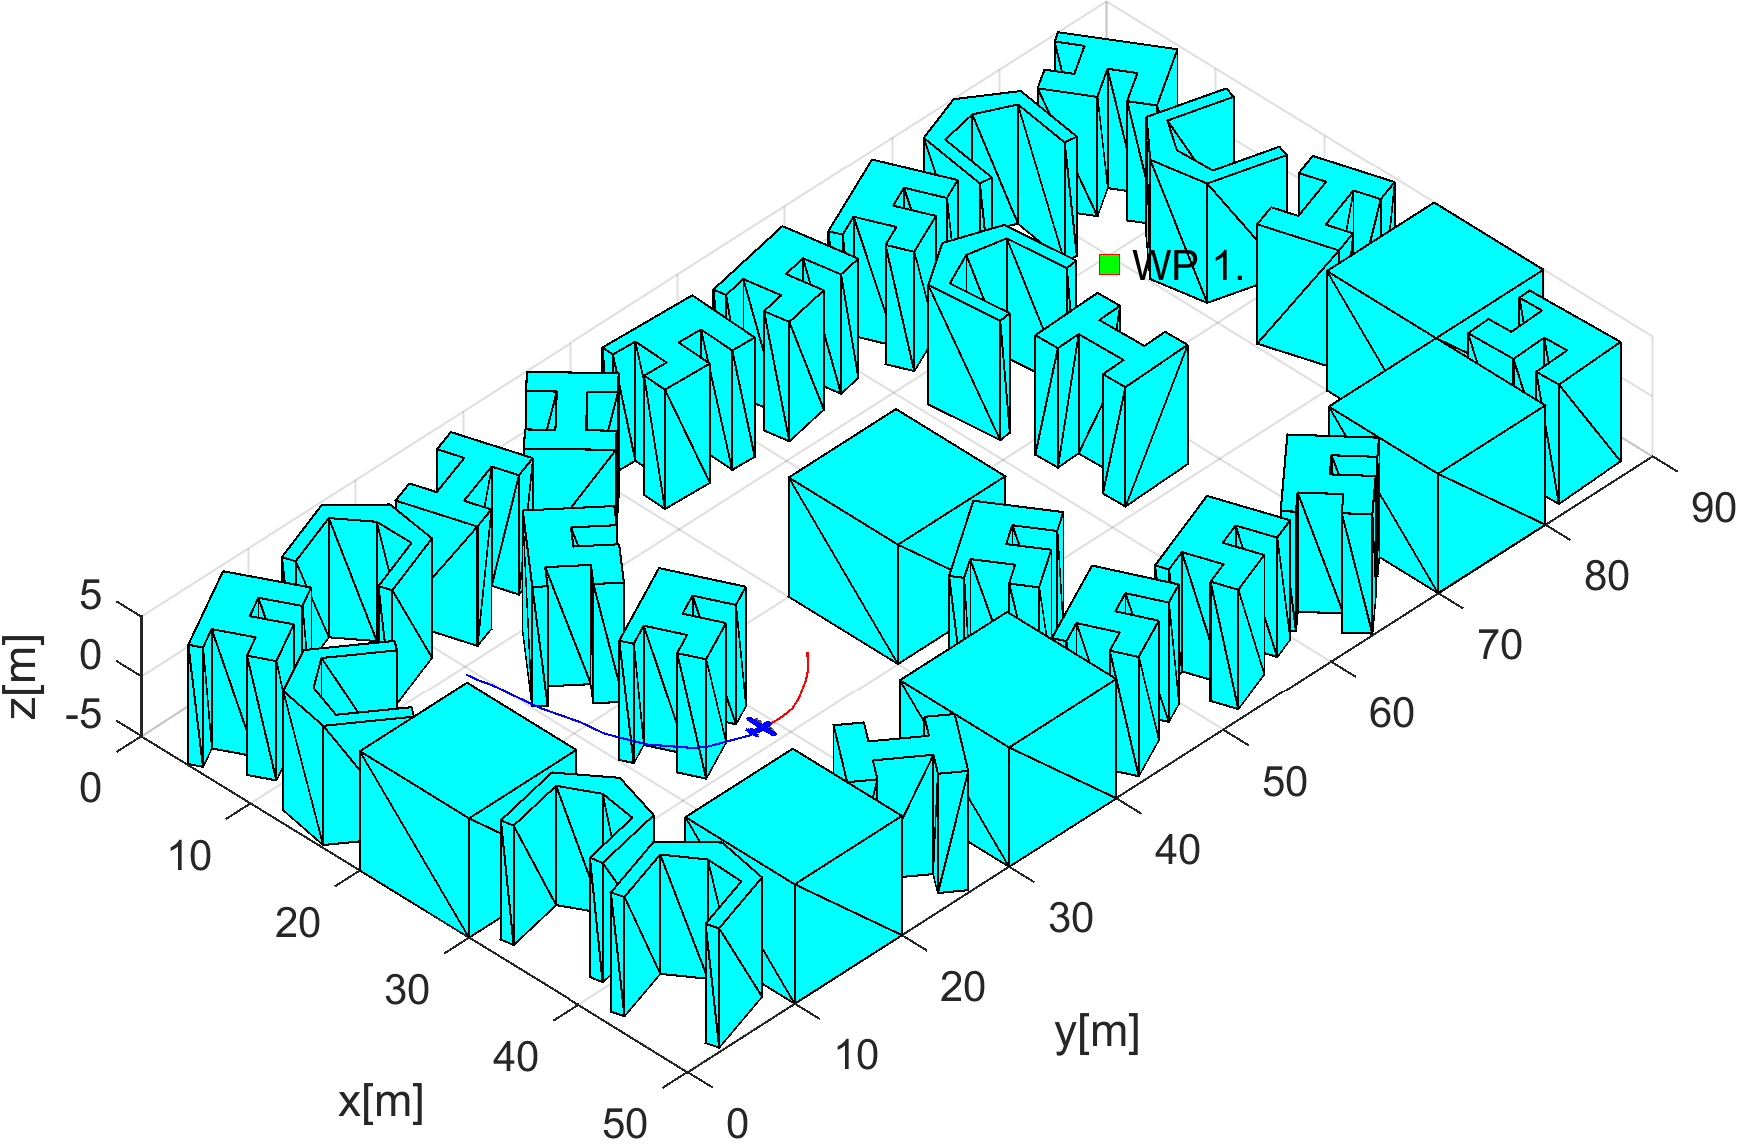
\includegraphics[width=0.9\linewidth]{\FIGDIR/NS013ConstraintsPolynomialMaze00022}
        \caption{$1^{st}$ turn.}
        \label{fig:mazeFirstTurn}
    \end{subfigure}
    \begin{subfigure}{0.48\textwidth}
	    \centering
        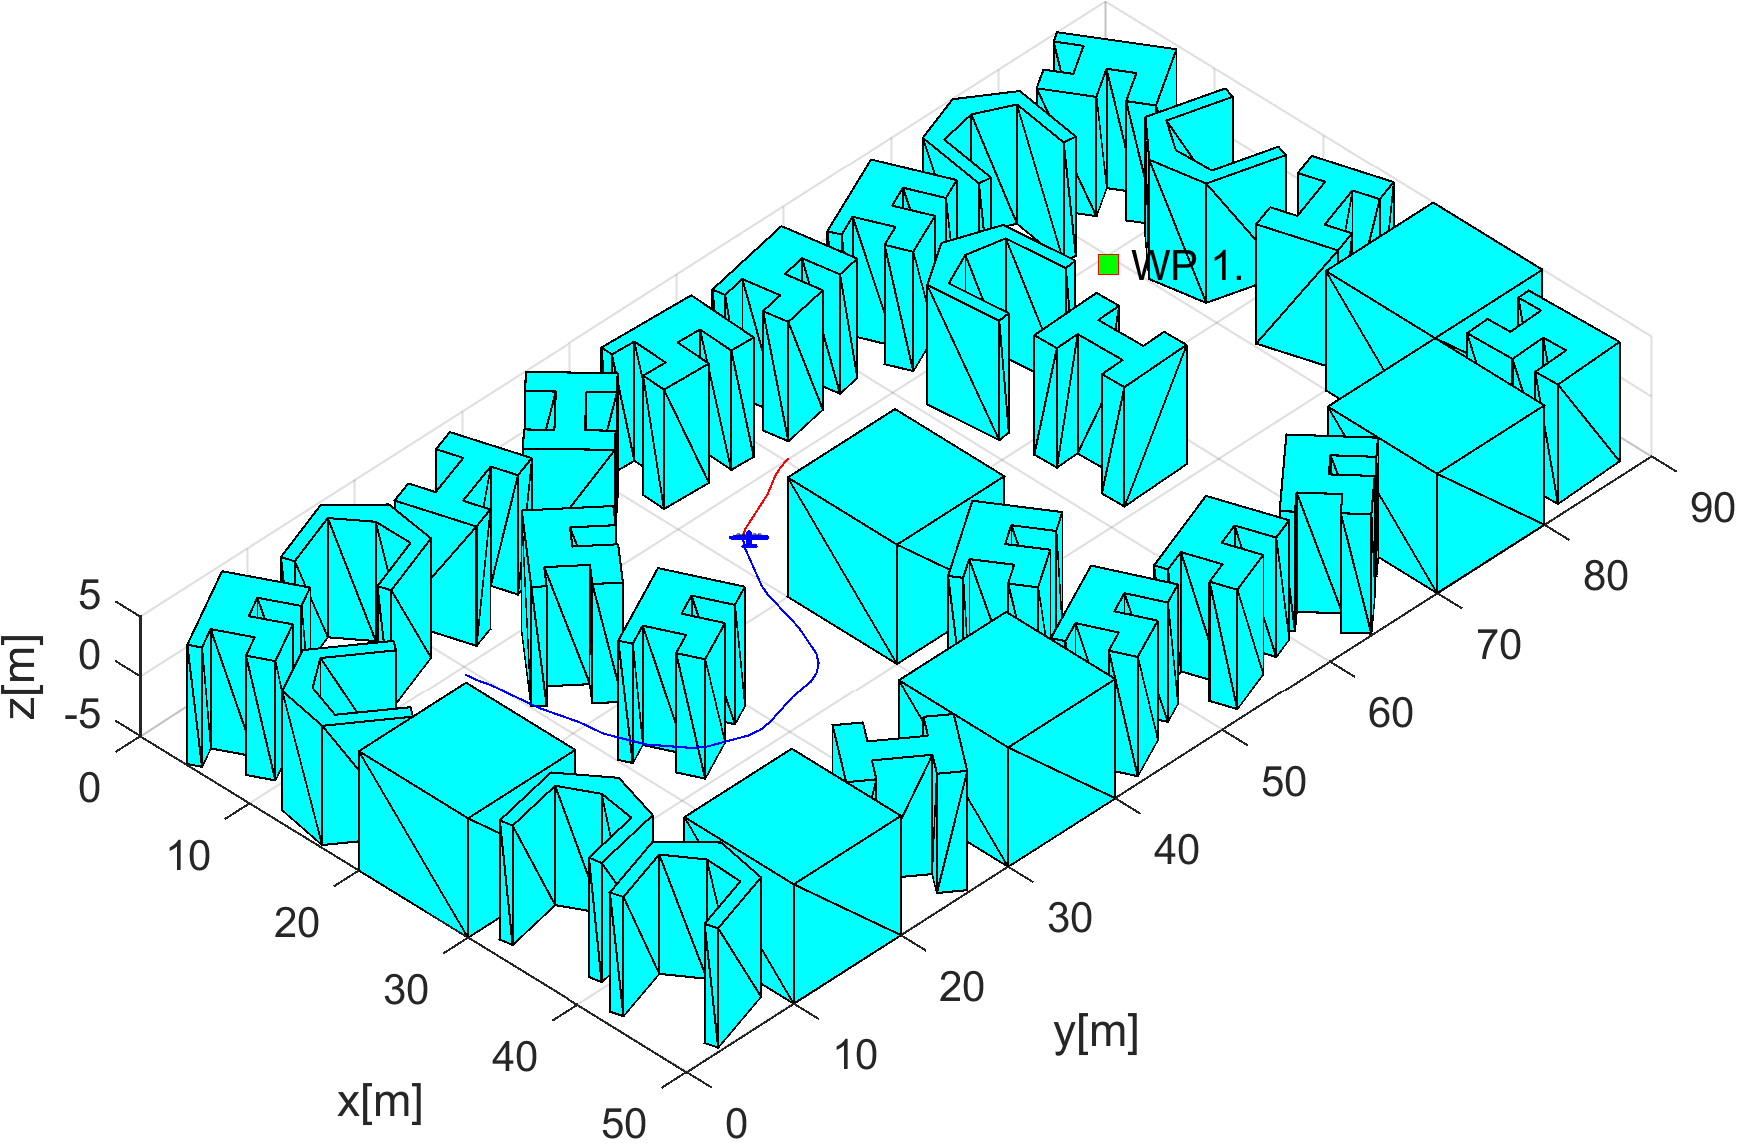
\includegraphics[width=0.9\linewidth]{\FIGDIR/NS014ConstraintsPolynomialMaze00044} 
        \caption{$2^{nd}$ turn.}
        \label{fig:mazeSecondTurn}
    \end{subfigure}
    \\
    \begin{subfigure}{0.48\textwidth}
    	\centering
        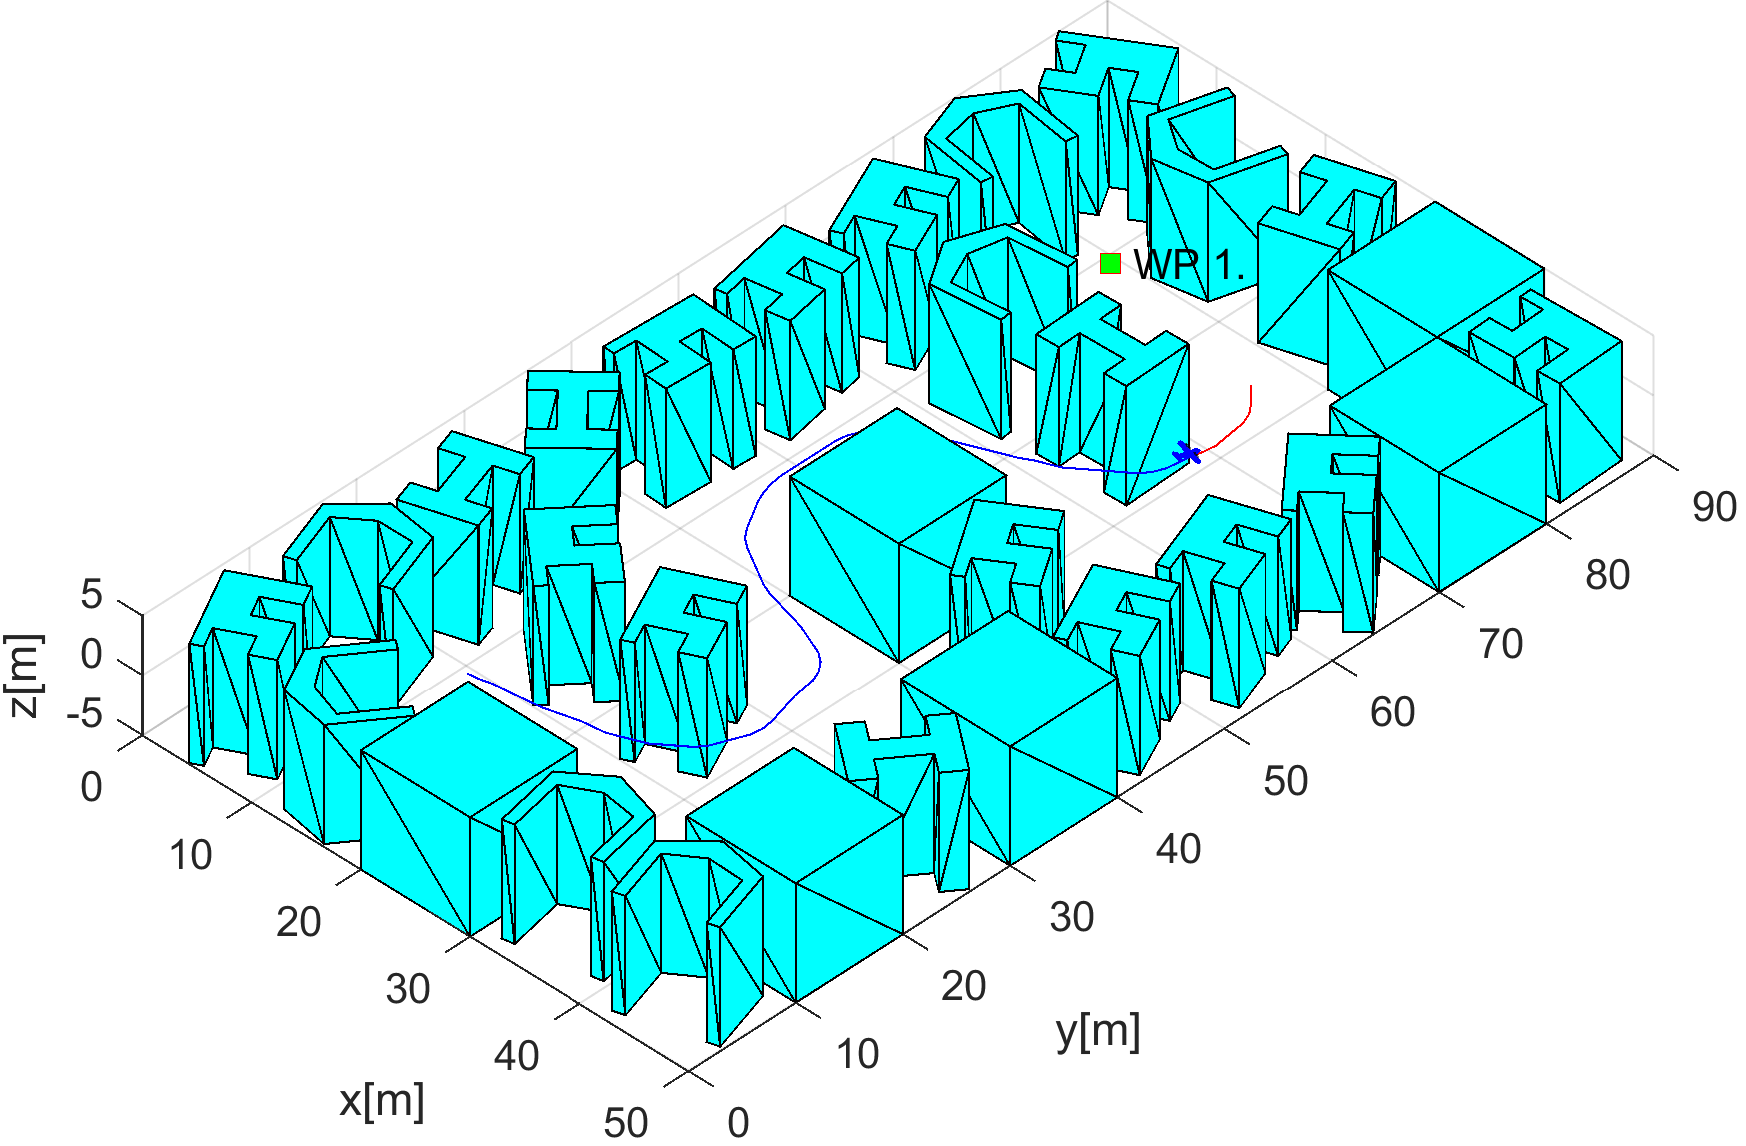
\includegraphics[width=0.9\linewidth]{\FIGDIR/NS015ConstraintsPolynomialMaze00081} 
        \caption{$3^{rd}$ turn.}
        \label{fig:mazeThirdTurn}
    \end{subfigure}
    \begin{subfigure}{0.48\textwidth}
    	\centering
        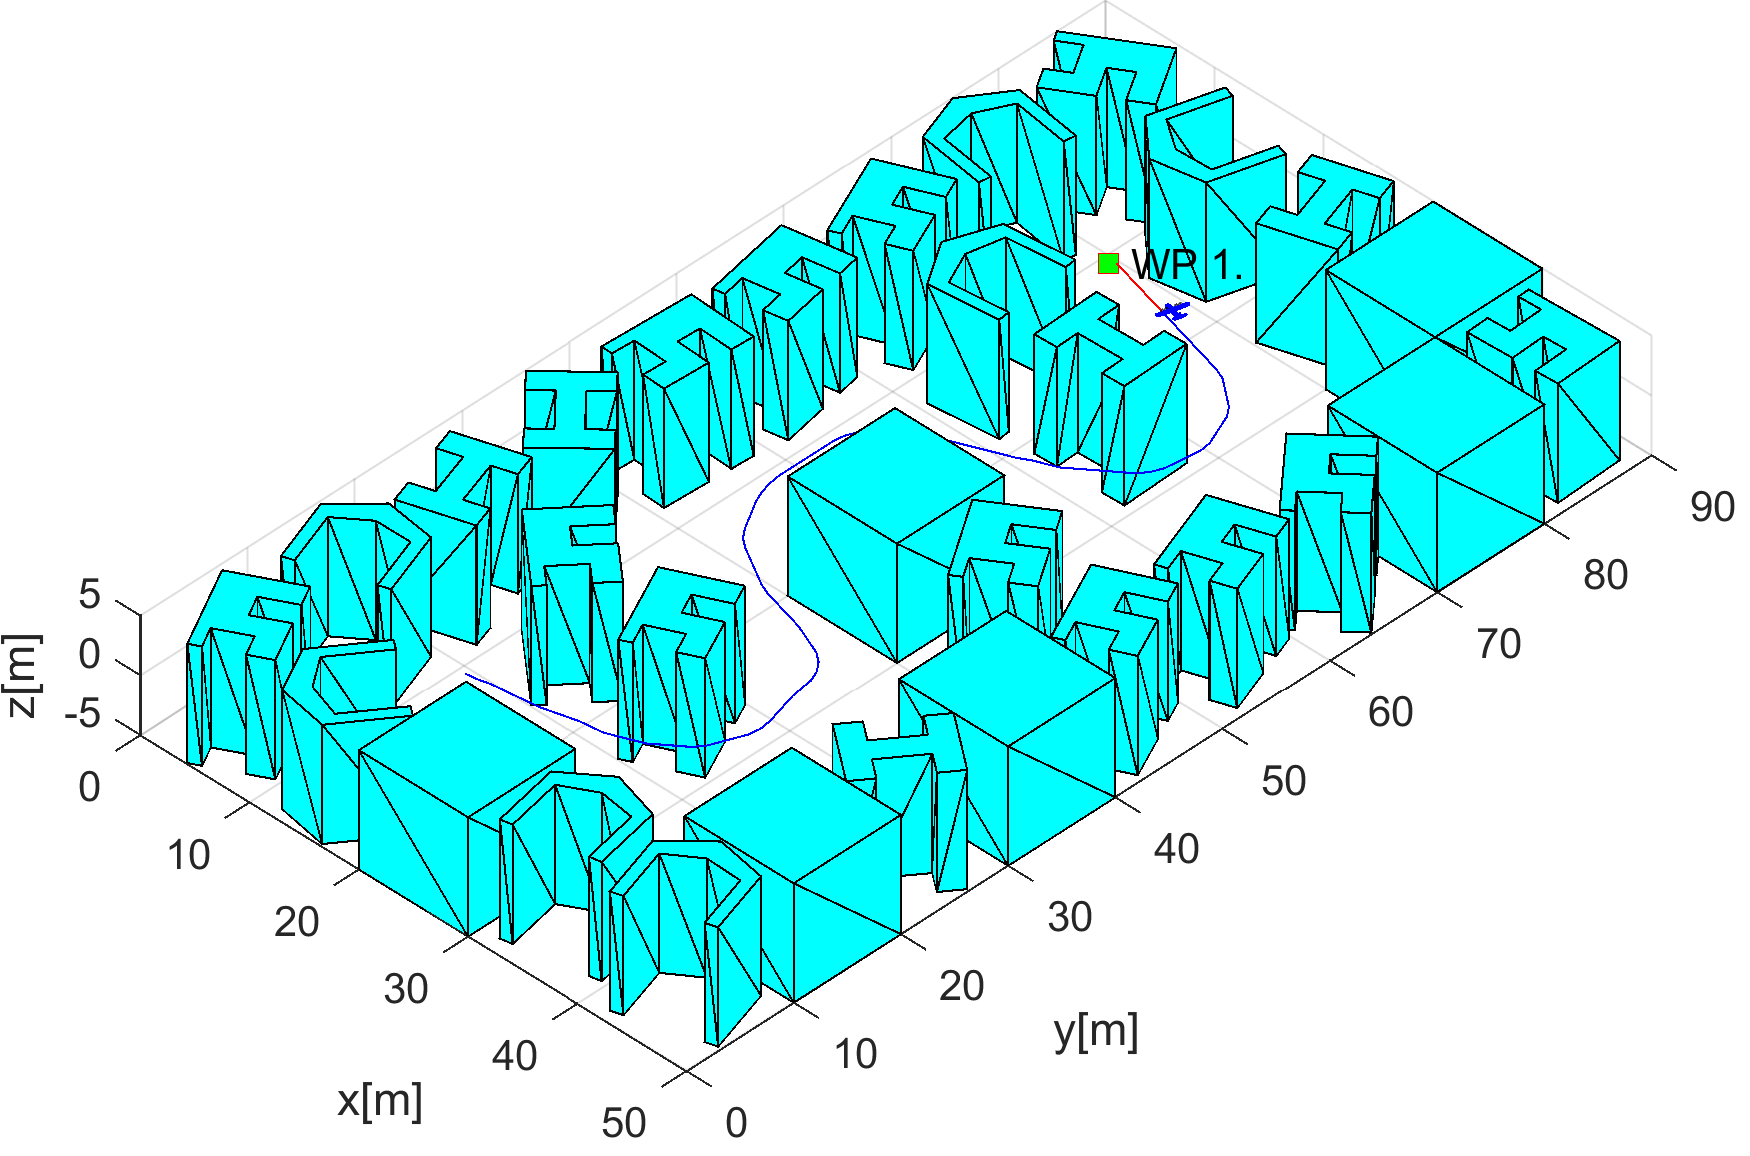
\includegraphics[width=0.9\linewidth]{\FIGDIR/NS016ConstraintsPolynomialMaze00098} 
        \caption{Waypoint reach.}
        \label{fig:mazeWaypointReach}
    \end{subfigure}
    \caption{Test scenario for \emph{Maze}. }
    \label{fig:testCaseMazeSolver}
\end{figure}

\paragraph{Distance to Body/Safety Margin Evolution:}  The evolution of \emph{body and safety margin} over time (x-axis, sec) given in  meters distance (y-axis, m) is given in (fig. \ref{fig:testCaseMazeAvoidancePerformance}).

The \emph{UAS} center distance to nearest obstacle (blue line) does not break any \emph{Safety Margin} (yellow line) of closest obstacle. \emph{Body Margin} of closest obstacle (red line) has not been break, because it always lies below of \emph{Safety Margin} (yellow).

For \emph{UTM time period} $37$ to $68$ sec there is a \emph{margin spike}  due avoidance of bloated \emph{Rectangle buildings} (fig. \ref{fig:mazeSecondTurn}) during $2^{nd}$ turn. The \emph{acceptance criterion} for \emph{Safety Margin} is satisfied.

\begin{note}
The \emph{body} and \emph{safety margin} are changing  depending on \emph{UAS position} and \emph{orientation}. The changes are reflected in (tab. \ref{tab:testCaseMazeSafetyAndBodyMarginDistances}).
\end{note}


\begin{figure}[H]
    \centering
    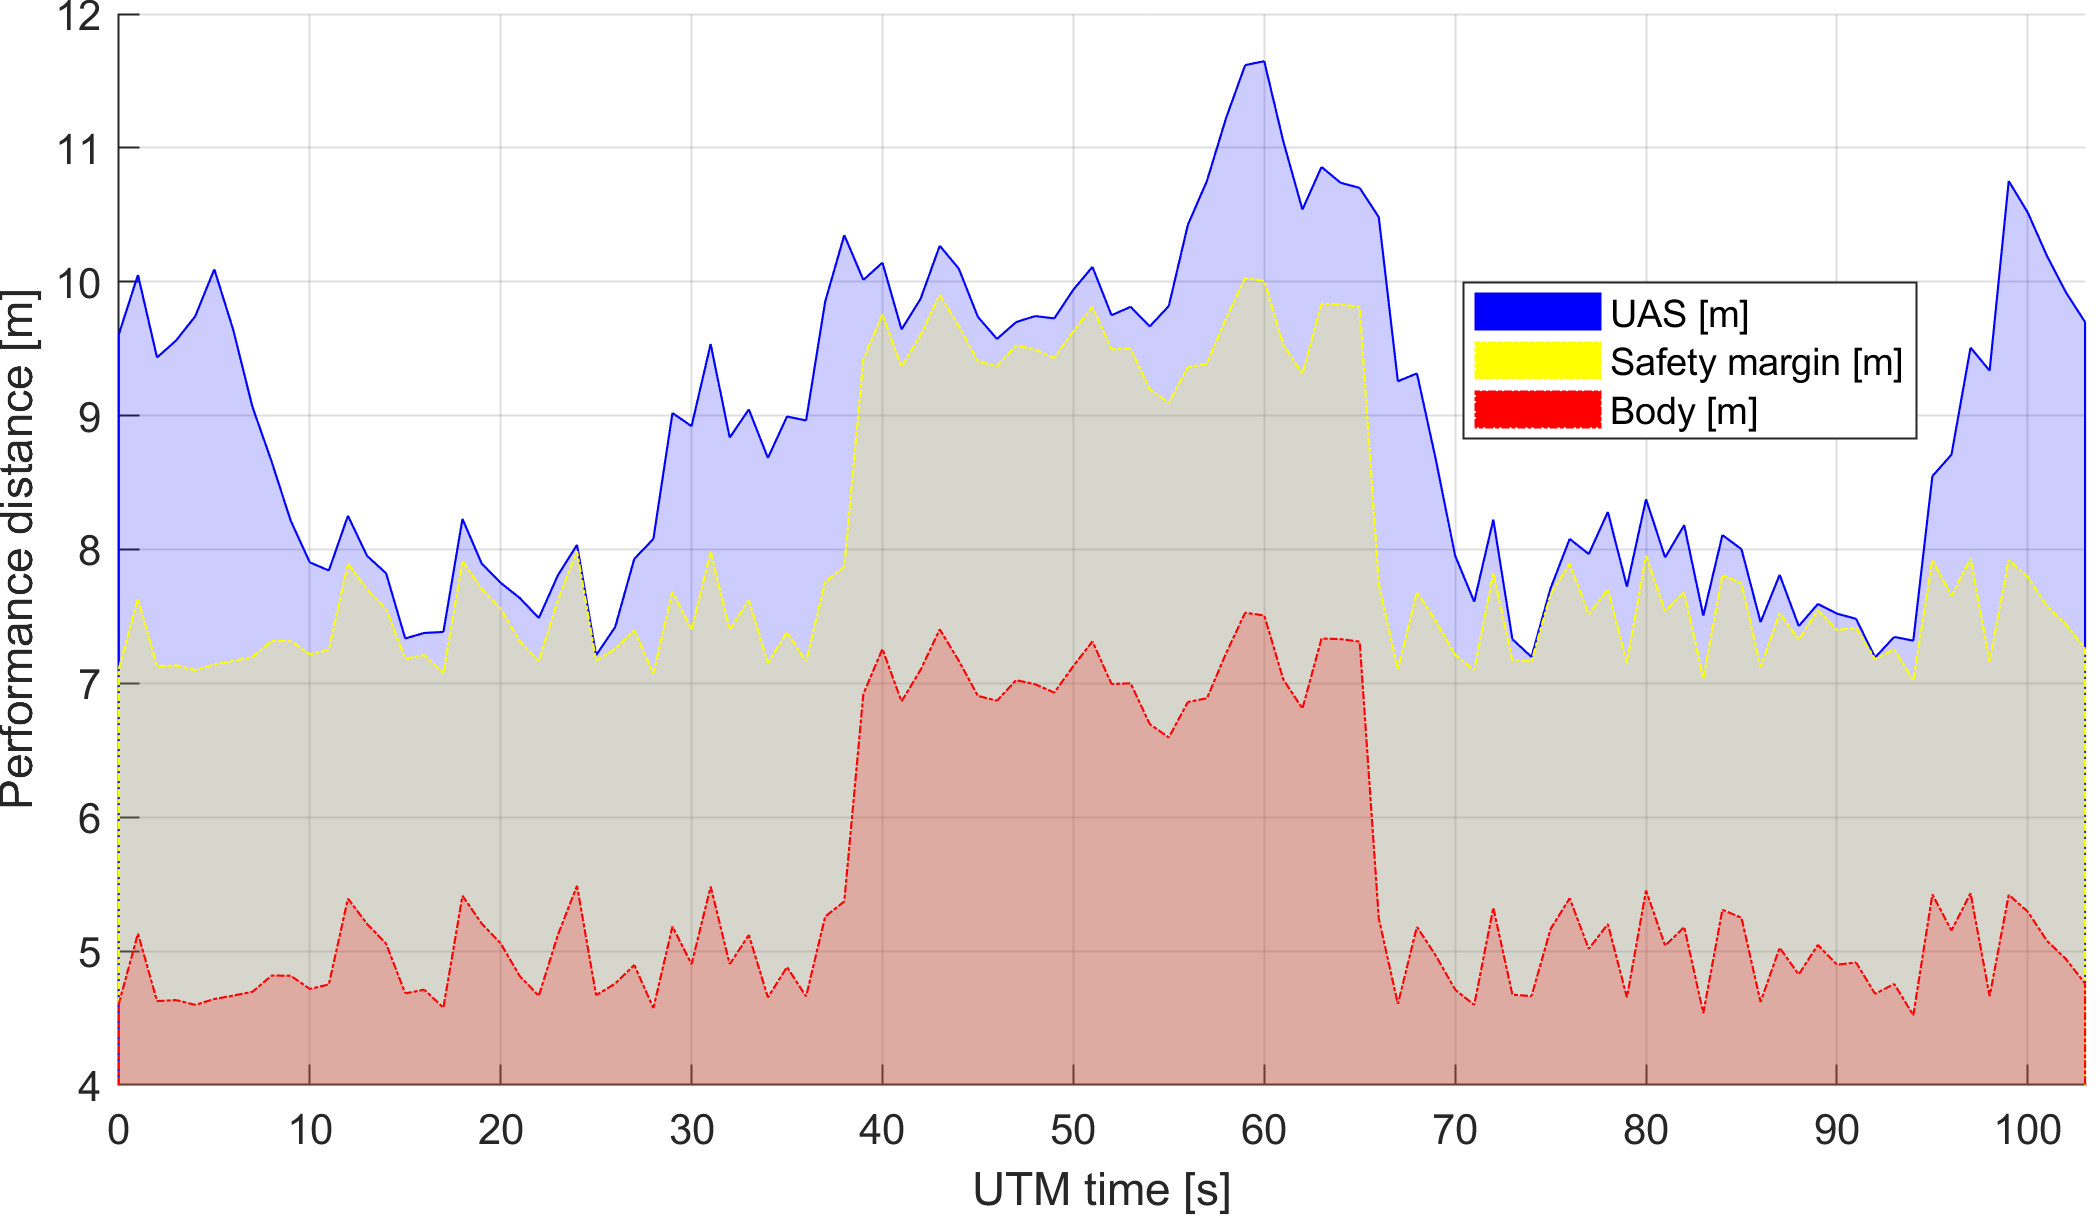
\includegraphics[width=0.8\linewidth]{\FIGDIR/NS017ConstraintsPolynomialMazePerformance} 
    \caption{Distance to body/safety margin evolution for \emph{Maze scenario}.}
    \label{fig:testCaseMazeAvoidancePerformance}
\end{figure}

\paragraph{Distance to Body/Safety Margin Peaks:} The minimal and maximal values for \emph{UAS distance} to \emph{safety margin} based on performance (fig. \ref{fig:testCaseMazeAvoidancePerformance}) is summarized in (tab. \ref{tab:testCaseMazeSafetyAndBodyMarginDistances}).

The \emph{minimal distance to safety margin} is $0.0131 m$ which can be taken as $\sim 0m$ due the numerical error. The \emph{maximal distance to safety margin} is $2.9513 m$ which is $5 \times$ \emph{UAS radius}. The safety margin distance is $\le 3 m$ which means the scenario is tightly packed with obstacles. The \emph{UAS} never left \emph{Emergency Avoidance Mode} because condition: $safety Margin Distance \ge avoidance Grid Length$ was never satisfied. 

The \emph{minimal body} distance is $5.0131 m$, while the \emph{maximal body} distance is $8.7117 m$. The difference between minimal and maximal body distance is $\sim 4 m$ which also indicates scenario packed with obstacles. 

\begin{table}[H]
    \centering
    \begin{tabular}{c|c||c}
    \multicolumn{2}{c||}{Parameter} & UAS 1 \\\hline\hline
    \multirow{2}{*}{Distance to Safety Margin} & min & 0.0131 \\\cline{2-3}
                                            & max & 2.9513 \\\hline
    \multirow{2}{*}{Distance to Body Margin}   & min & 5.0131 \\\cline{2-3}
                                            & max & 8.7117 
    \end{tabular}
    \caption{Distance to body/safety margin peaks for \emph{Maze scenario}.}
    \label{tab:testCaseMazeSafetyAndBodyMarginDistances}
\end{table}

\paragraph{Path Tracking Performance:} Reference path (green dashed) line is given as direct interconnection of \emph{initial position} (green square with S marker) and \emph{hidden waypoint} (green square with 1 marker). The \emph{UTM Reference Time} is given on x-axis. The evolution of real trajectory (blue solid line) for each axis is given as follow:

\begin{enumerate}
    \item \emph{X-axis path tracking} - reflects the maneuvering in the curves of the maze.
    
    \item \emph{Y-axis path tracking} - shows horizontal progress to the \emph{hidden goal waypoint}. The expected linear tracking is not achievement due the manuevering delays on X-axis.
    
    \item \emph{Z-axis path tracking} - shows perfect linear tracking of reference trajectory. The \emph{altitude acceptance criterion}: $-5m \le altitude \le 5m$ have been fulfilled.
\end{enumerate}

\begin{figure}[H]
    \centering
    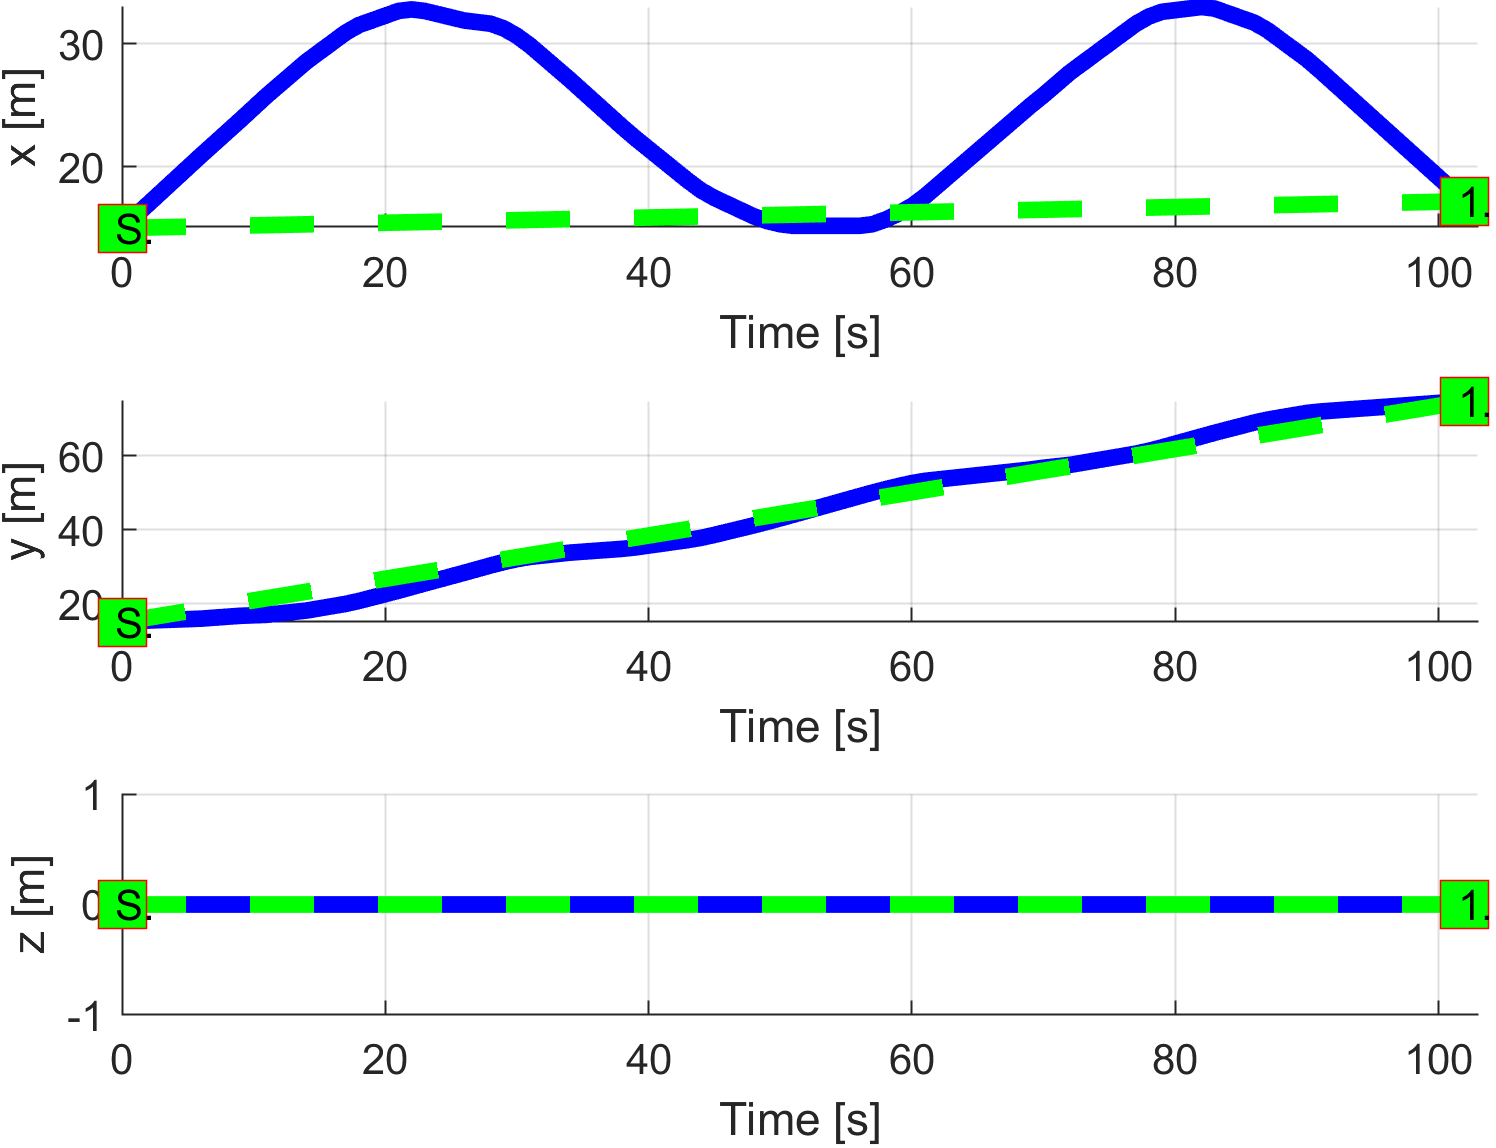
\includegraphics[width=0.55\linewidth]{\FIGDIR/NS018ConstraintsPolynomialMazePathFollowing} 
    \caption{\emph{Maze} path tracking.}
    \label{fig:testCaseMazePathTracking}
\end{figure}


\paragraph{Path Tracking Deviations:} Deviations (tab. \ref{tab:pathTrackingParametersForMazeAvoidance}) from \emph{reference trajectory} are in expected ranges considering \emph{mission plan} (tab. \ref{tab:missionSetupMazeScenario}) and \emph{obstacle properties} (tab. \ref{tab:obstacleSetMaze}).

\begin{table}[H]
    \centering
    \begin{tabular}{c||c}
        \multirow{2}{*}{Param.} & UAS 1\\\cline{2-2}
                        & $\mathscr{WP}_1$  \\\hline\hline
          $\max |x|$    & 27.32             \\\hline
          $\max |y|$    & 2.41             \\\hline
          $\max |z|$    & 0                 \\\hline
          $\max dist.$  & 28.06             \\
    \end{tabular}
    \caption{Path tracking properties for \emph{Maze} scenario.}
    \label{tab:pathTrackingParametersForMazeAvoidance}
\end{table}



    	\subsection{Storm}\label{s:testStorm}
    \paragraph{Scenario:} Small UAS is flying in open space in uncontrolled airspace ($\le$ 500 feet AGL (Above Ground Level)). A \emph{Weather Service} notices UAS about \emph{Dangerous Weather zone} (virtual constraint s. \ref{s:virtualConstraints}) which is moving in UAS direction. The \emph{UAS} is  executing mission given by (tab. \ref{tab:missionSetupStormScenario}).
    
    \begin{table}[H]
        \centering
        \begin{tabular}{c|c||c}
            \multicolumn{2}{c||}{Position} & \multirow{2}{*}{$\mathscr{WP}_1$} \\\cline{1-2}
            $[x,y,z]$           & $[\theta,\varpi,\psi]$           & \\\hline\hline
            $[0,0,0]^T $        & $[0^\circ,0^\circ,90^\circ]^T$    & $[0,60,0]^T$        \\ 
        \end{tabular}
        \caption{Mission setup for \emph{Storm} scenario.}
        \label{tab:missionSetupStormScenario}
    \end{table}
    
    \paragraph{Constraints:} The \emph{storm} is modeled as a \emph{virtual constraint} with parameters given in (tab. \ref{tab:obstacleSetStorm}). A constraint is modeled as a \emph{convex polygon} for \emph{horizontal boundary} and altitude for the \emph{vertical boundary}.
    
    The \emph{Storm} is moving through an \emph{operational region} with linear velocity $0.5 ms^{-1}$. The \emph{storm`s center} was first detected at \emph{decision frame} $0$ at position $[0,50,0]^T$.
    
    \begin{table}[H]
        \centering
        \begin{tabular}{c|c|c|c|c|c|c}
            \multicolumn{3}{c|}{Constraint} & \multicolumn{3}{c|}{Body Margin} & \multirow{2}{*}{Safety Margin}\\\cline{1-6}
            i. position & velocity & type & min. & max. & avg. &   \\\hline\hline
            $[0,50,0]^T$ & $[0,-0.5,0]$ & polygon & $9$ & $10$ & $9.5$  & $5$ \\
         \end{tabular}
        \caption{\emph{Constraint set} for \emph{Storm} scenario.}
        \label{tab:obstacleSetStorm}
    \end{table}
    
    \paragraph{Assumption:} Every \emph{avoidable moving constraint} is usually slower than an \emph{Approaching UAS}, or its radius is smaller than the turning radius of an \emph{Approaching UAS}.
    
    \begin{note}
    \emph{Manned aviation} receives a permit to operate in  \emph{controlled airspace} only if it has capability outmaneuver every known threat in requested airspace. 
    
    The \emph{Constrained space portion} is usually very large, therefore in the majority of cases the assumption $uasSpeed >> constraintSpeed$  holds.
    \end{note}
 
    \paragraph{Main Goal:} Show dynamic moving constraint avoidance capability in \emph{uncontrolled airspace}.
    
    \paragraph{Acceptance criteria:}
    \begin{enumerate}
        \item \emph{Hard constraint avoidance} - the \emph{UAS} must not cross the body margin:  $distance($ $stormCenter,$ $UAS)$ $\ge$  $bodyMargin$.
        
        \item \emph{Soft constraint avoidance} - the \emph{UAS} cannot cross the safety margin to get into proximity of \emph{Storms surrounding area}: \emph{distance(stormCenter, UAS)} $\ge$ \emph{safetyMargin}. 
    \end{enumerate}
    
    \paragraph{Testing setup:} The \emph{standard test setup} defined in (tab. \ref{tab:testMovementOrientations}, \ref{tab:testUASBasicParameters}, \ref{tab:testNavigationGridBasic}, \ref{tab:testAvoidanceGridBasic}, \ref{tab:testUASColoring}) is used with following parameter override:
    \begin{enumerate}
        \item \emph{Avoidance grid - type} - \emph{ACAS-like} with \emph{horizontal enabled maneuvers}.
    \end{enumerate}
    
    \paragraph{Simulation run:} \emph{Notable moments} from a \emph{simulation run} (fig. \ref{fig:testCaseStormAvoidance}) are the following:
    \begin{enumerate}
    
        \item \emph{Detection} (fig. \ref{fig:stromSituationDetection}) - the \emph{Storm} (magenta polygon) is detected prior to the engagement (retrieved from associated weather service). The \emph{UAS} (blue) stays in \emph{Navigation mode}. \emph{Trajectories} in \emph{Navigation grid} are constrained by rule \emph{Enforce safety margin} (tab. \ref{tab:ruleEnforceSafetyMargin}). The \emph{Planned trajectory} (red) changes to avoid \emph{Storm}.
        
        \item \emph{Avoidance start} (fig. \ref{fig:stormAvoidanceStart}) - when UAS reaches optimal avoidance distance, the \emph{navigation reach set} is constrained, forcing UAS to perform an evasive maneuver.
        
        \item \emph{Avoidance end} (fig. \ref{fig:stormAvoidanceEnd}) - navigation space is no longer constrained when the \emph{minimal safe distance/heading} is achieved.
        
        \item \emph{Waypoint reached} (fig. \ref{fig:stormWaypointReach}) - standard waypoint navigation procedure was used in this case.
        
    \end{enumerate}
        
    \begin{figure}[H]
        \centering
        \begin{subfigure}{0.48\textwidth}
        	\centering
            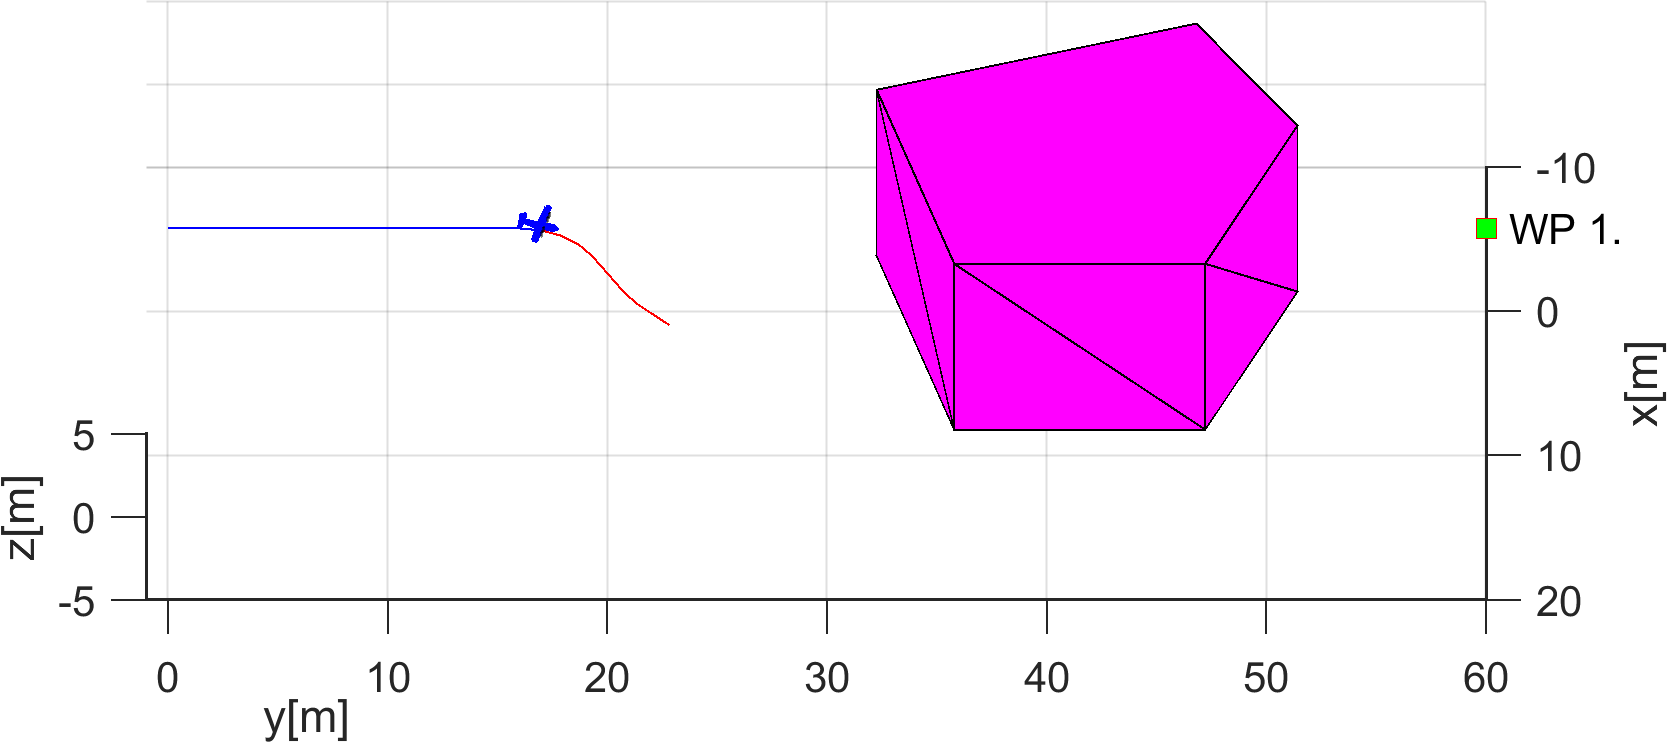
\includegraphics[width=0.9\linewidth]{\FIGDIR/NS019ConstraintsPolynomialStorm00017}
            \caption{Situation detection.}
            \label{fig:stromSituationDetection}
        \end{subfigure}
        \begin{subfigure}{0.48\textwidth}
        	\centering
            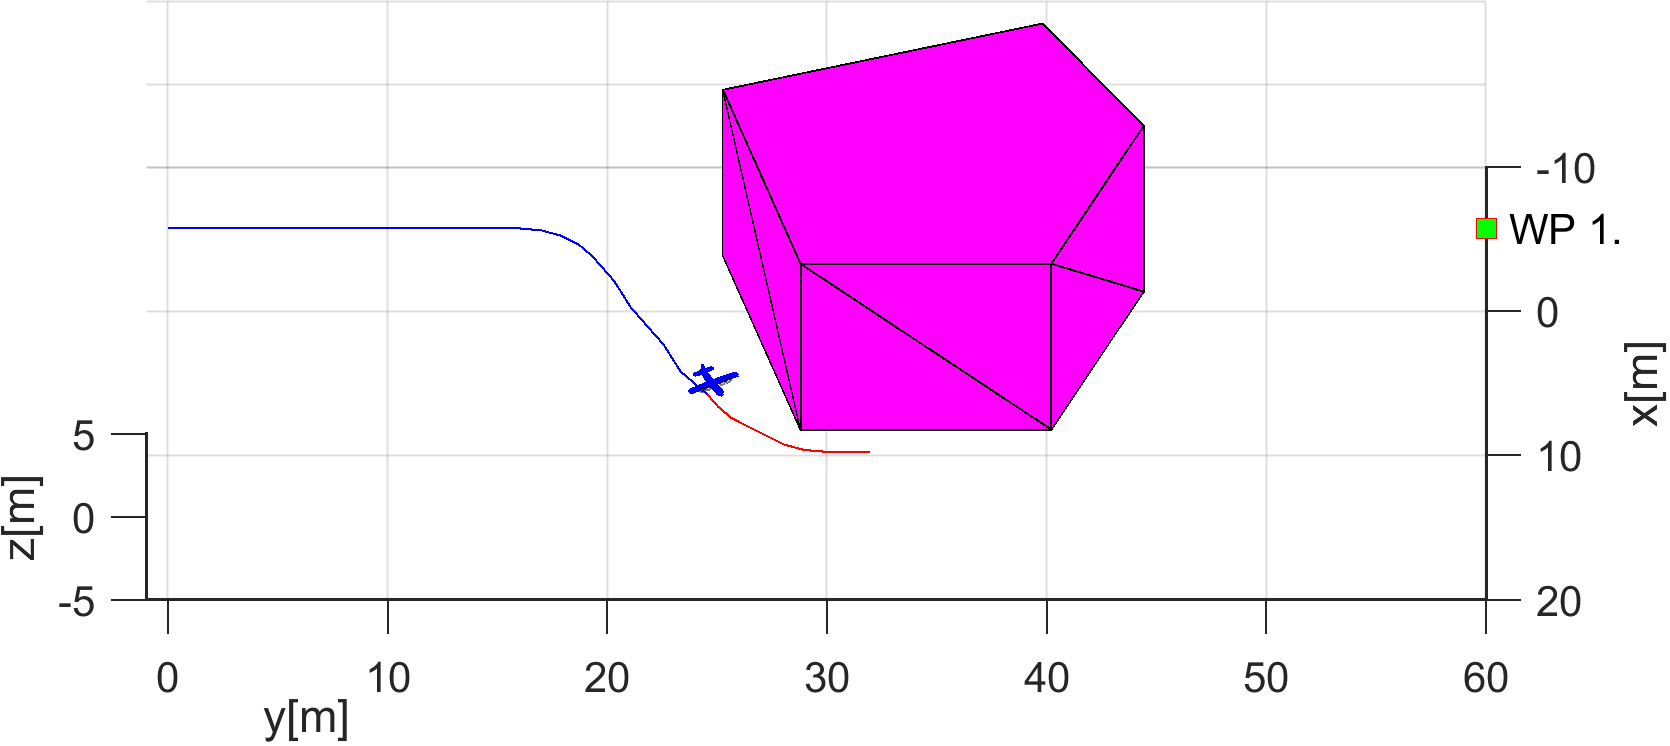
\includegraphics[width=0.9\linewidth]{\FIGDIR/NS020ConstraintsPolynomialStorm00031} 
            \caption{Storm avoidance start.}
            \label{fig:stormAvoidanceStart}
        \end{subfigure}
        \\
        \begin{subfigure}{0.48\textwidth}
        	\centering
            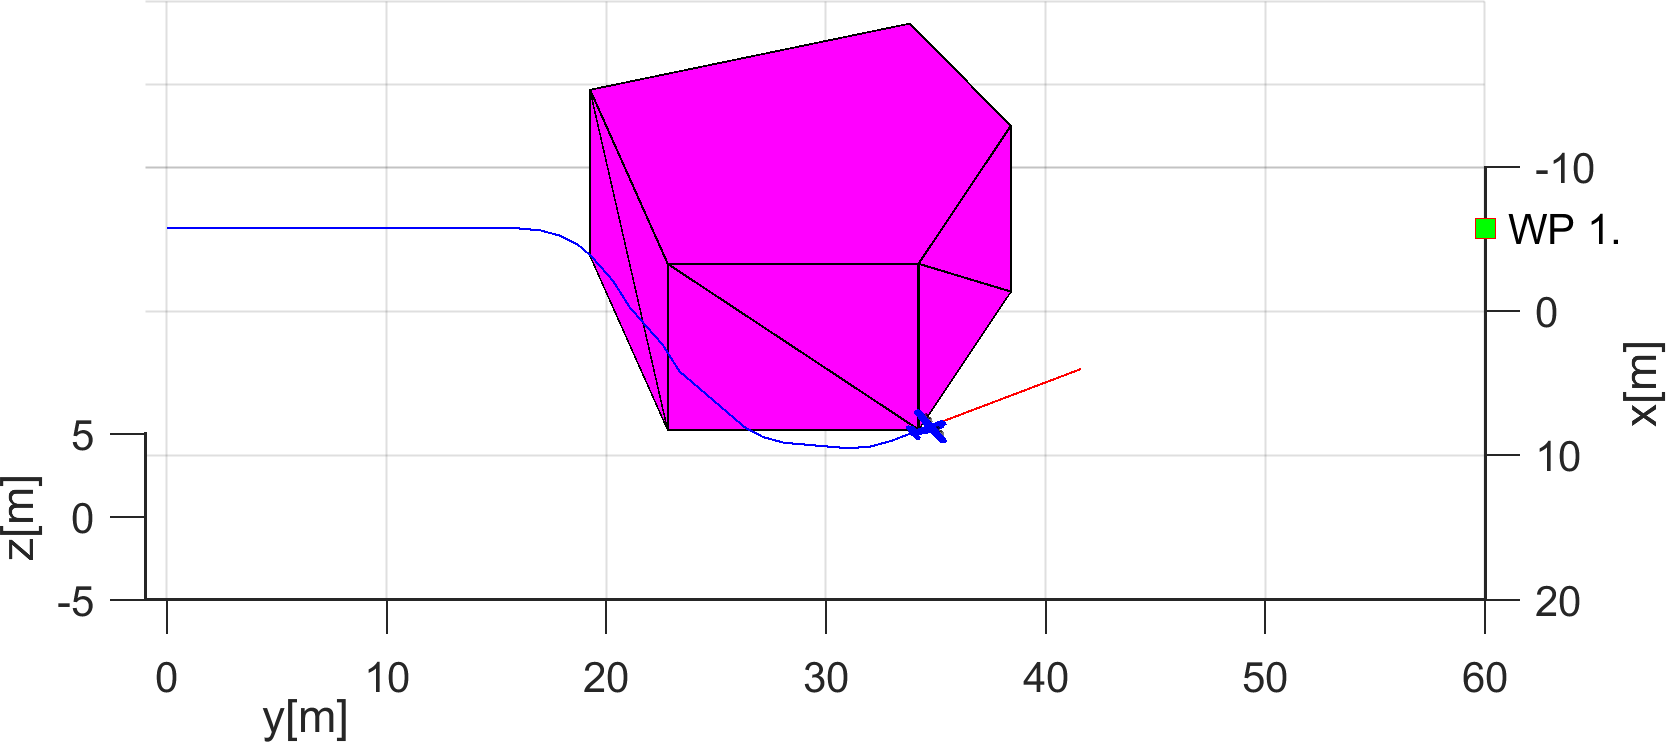
\includegraphics[width=0.9\linewidth]{\FIGDIR/NS021ConstraintsPolynomialStorm00043} 
            \caption{Storm avoidance end.}
            \label{fig:stormAvoidanceEnd}
        \end{subfigure}
        \begin{subfigure}{0.48\textwidth}
        	\centering
            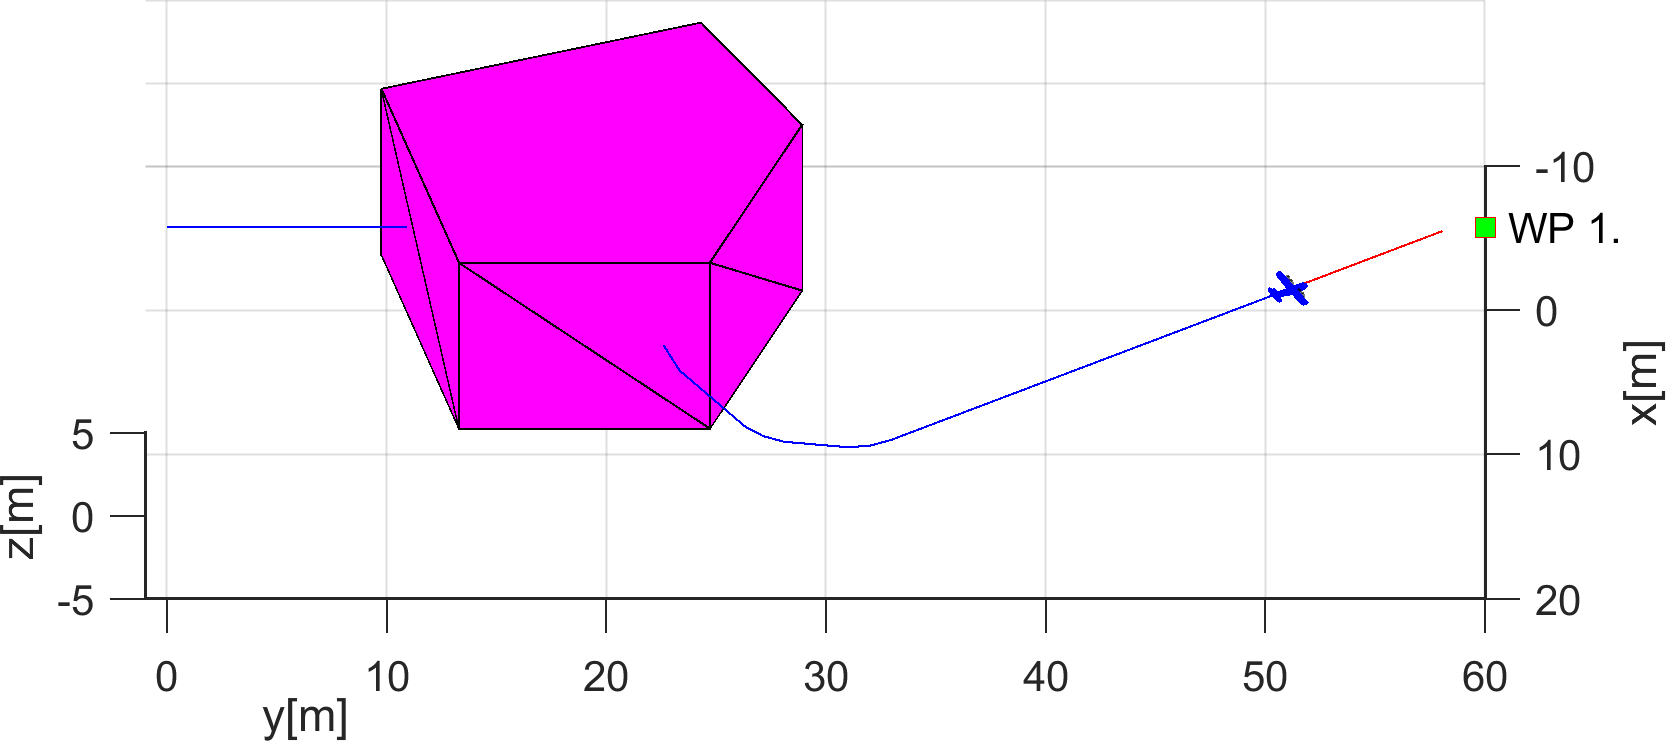
\includegraphics[width=0.9\linewidth]{\FIGDIR/NS022ConstraintsPolynomialStorm00062} 
            \caption{Waypoint reach.}
            \label{fig:stormWaypointReach}
        \end{subfigure}
        \caption{Test scenario for \emph{Storm} (Dynamic hard constraint). }
        \label{fig:testCaseStormAvoidance}
    \end{figure}
    
    \paragraph{Distance to Body/Safety Margin Evolution:} The \emph{body margin} (red line) and \emph{safety margin} (yellow line) and \emph{UAS distance to storm center} (blue line) evolution over \emph{UTM time} (x-axis) are given in (fig. \ref{fig:testCaseStormAvoidancePerformance}) The \emph{body} and \emph{safety} margin was changing according to the mutual position of the \emph{storm} and the \emph{UAS} (see tab. \ref{tab:obstacleSetStorm}). 
    
    The acceptance criteria for the \emph{hard constraint avoidance} and \emph{soft constraint avoidance} have been fulfilled. 
    
    \begin{figure}[H]
        \centering
        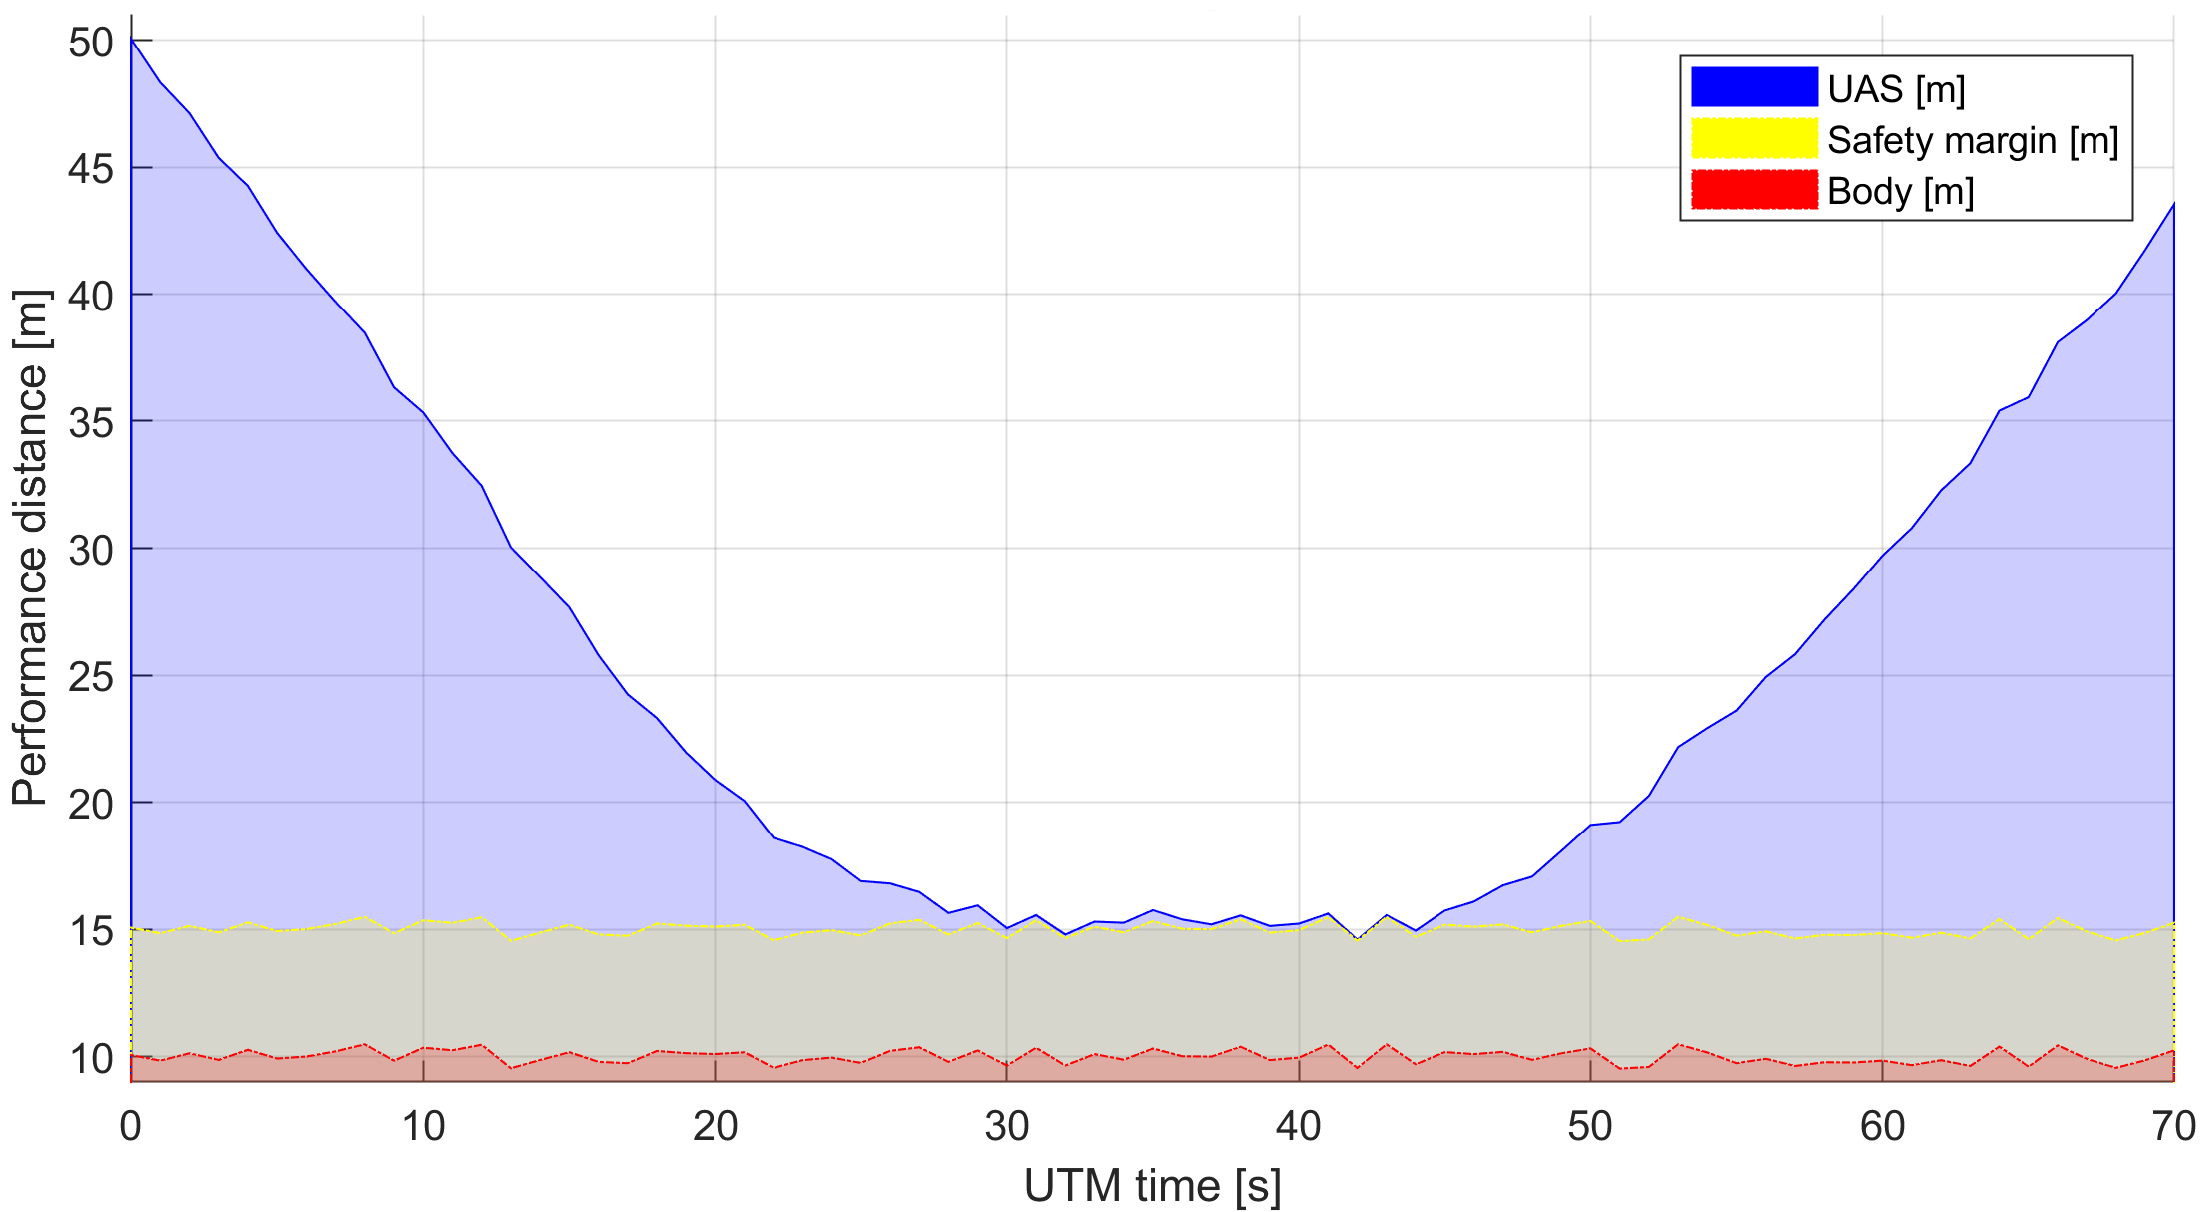
\includegraphics[width=0.8\linewidth]{\FIGDIR/NS023ConstraintsPolynomialStormPerformance} 
        \caption{Distance to body/safety margin evolution for \emph{Storm scenario}.}
        \label{fig:testCaseStormAvoidancePerformance}
    \end{figure}
    
    
    \paragraph{Distance to Body/Safety Margin Peaks:} A \emph{hard constraint} of \emph{body margin} was not breached, because the \emph{distance(UAS(t),stormBody(t))} was all time greater than \emph{0}. Thus the \emph{UAS} stayed well clear from \emph{Storm}. The summary (tab. \ref{tab:testCaseStormSafetyAndBodyMarginDistances}) shows that the \emph{minimal body margin distance} was $5.0335$ $m$, which proves \emph{avoidance of hard constraint}.
    
    A \emph{soft constraint} represented as a \emph{safety margin} (protective coating around storm body) was not breached, because the \emph{distance(UAS(t), stormBody(t)) - safetyMargin(t)} was all time greater than \emph{0}.  The summary (tab. \ref{tab:testCaseStormSafetyAndBodyMarginDistances}) show that the \emph{minimal safety margin distance} was $0.0355$ $m$, which proves \emph{avoidance of soft constraints}.
    
    \begin{table}[H]
        \centering
        \begin{tabular}{c|c||c}
        \multicolumn{2}{c||}{Parameter} & UAS 1 \\\hline\hline
        \multirow{2}{*}{Distance to Safety Margin} & min & 0.0355 \\\cline{2-3}
                                                & max & 34.9934 \\\hline
        \multirow{2}{*}{Distance to Body Margin}   & min & 5.0355 \\\cline{2-3}
                                                & max & 39.9934 
        \end{tabular}
        \caption{Distance to body/safety margin peaks for \emph{Storm scenario}.}
        \label{tab:testCaseStormSafetyAndBodyMarginDistances}
    \end{table}
    
    \paragraph{Path Tracking Performance:} The \emph{path tracking} (solid blue line) of \emph{reference trajectory} (green dashed line) between \emph{starting waypoint} (green square marked "S") and \emph{final waypoint} (green square marked "1") is portrayed in (fig. \ref{fig:testCaseStormPathTracking}). The\emph{UAS} executes \emph{horizontal right-side avoidance} of the \emph{Storm} as is preferred. 
    
    \begin{figure}[H]
        \centering
        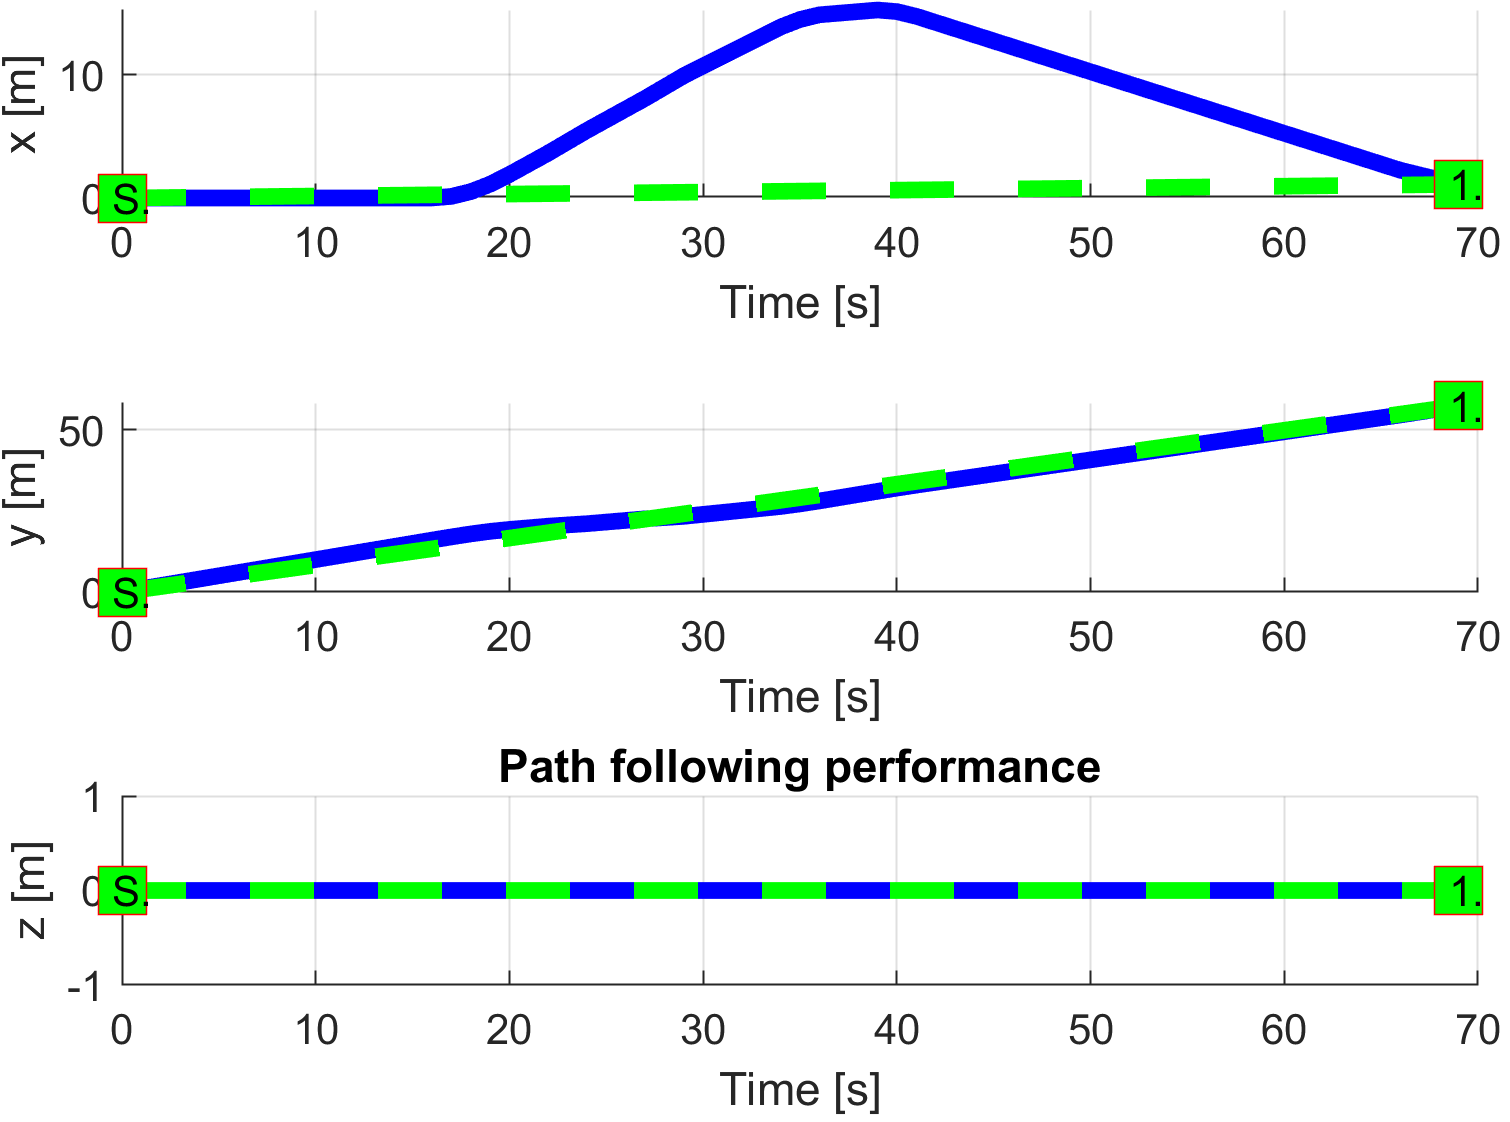
\includegraphics[width=0.55\linewidth]{\FIGDIR/NS024ConstraintsPolynomialStormPathFollowing} 
        \caption{\emph{Storm} avoidance scenario path tracking.}
        \label{fig:testCaseStormPathTracking}
    \end{figure}
    
    \paragraph{Path Tracking Deviations:} \emph{Deviations} (tab. \ref{tab:pathTrackingParametersForStormAvoidance}) are in expected ranges considering the mission plan (tab. \ref{tab:missionSetupStormScenario}) and \emph{body} and \emph{safety} margins (tab. \ref{tab:obstacleSetStorm}).
    
    \begin{table}[H]
        \centering
        \begin{tabular}{c||c}
            \multirow{2}{*}{Param.} & UAS 1\\\cline{2-2}
                            & $\mathscr{WP}_1$  \\\hline\hline
              $\max |x|$    & 15.26             \\\hline
              $\max |y|$    & 1.32             \\\hline
              $\max |z|$    & 0                 \\\hline
              $\max dist.$  & 15.76             \\
        \end{tabular}
        \caption{Path tracking properties for \emph{Storm} scenario.}
        \label{tab:pathTrackingParametersForStormAvoidance}
    \end{table}
    
    
    % 04 Storm
\paragraph{Computation Load:} The \emph{computation load} for \emph{scenario} (fig.\ref{fig:stormComputationTime}) shows used time (y-axis) over decision frame (x-axis).

The \emph{computation time} is low; it only increases slightly during  avoidance maneuver.

\begin{figure}[H]
    \centering
    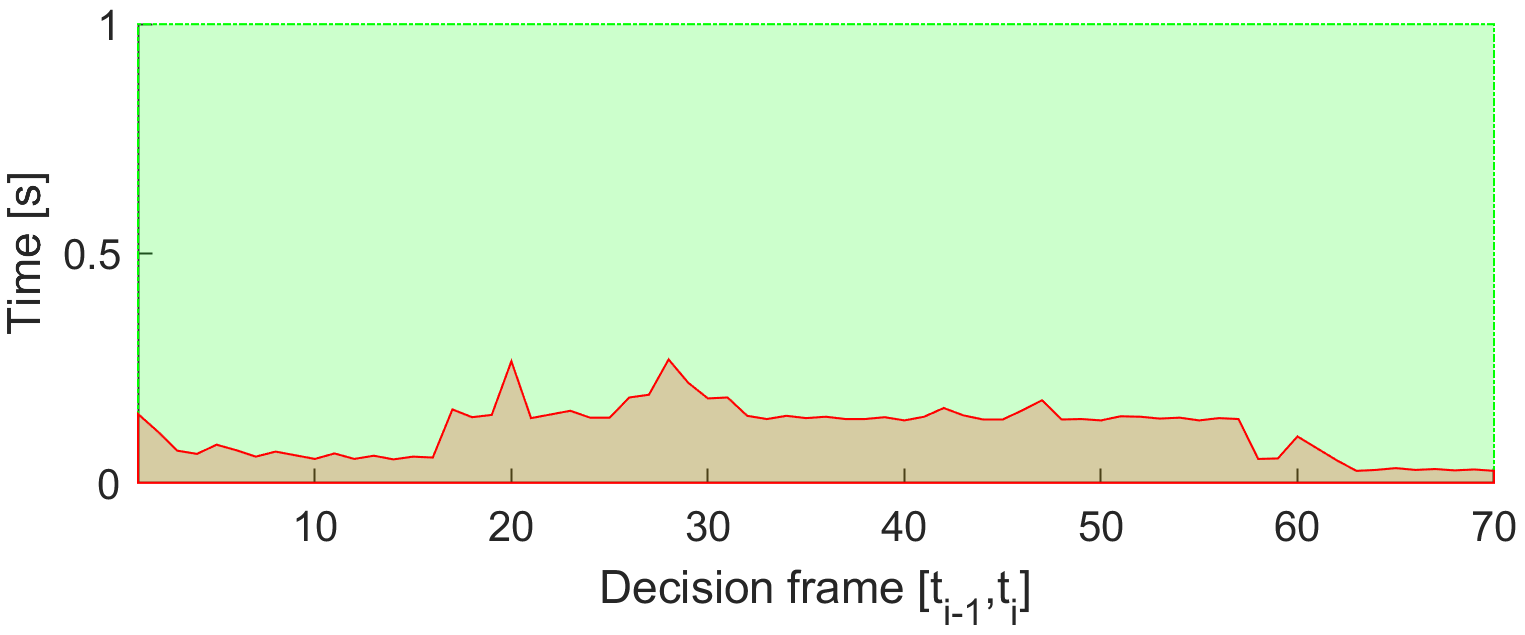
\includegraphics[width=0.65\linewidth]{\FIGDIR/NS095StormComputationTime} 
    \caption{Computation time for \emph{Maze} scenario.}
    \label{fig:stormComputationTime}
\end{figure}
    
    

    	\subsection{Emergency Converging}\label{s:testEmergencyConverging}

\paragraph{Scenario:} Two \emph{UAS} are flying in  \emph{uncontrolled airspace} (altitude $\le$ 500 ft. Above the Ground Level) with missions defined in (tab. \ref{tab:missionSetupEmergencyConvergingScenario}). Both \emph{UAS} are in the \emph{Navigation mode} with active \emph{ADSB-In/Out}, receiving position notification from each other. Cruising altitude is sufficient for horizontal separation (50-100 ft. Above the Ground Level). \emph{Horizontal separation} is the preferred separation type for both \emph{UAS}.

\begin{table}[H]
    \centering
    \begin{tabular}{c||c|c||c}
        \multirow{2}{*}{UAS} &\multicolumn{2}{c||}{Position} & \multirow{2}{*}{$\mathscr{WP}_1$} \\\cline{2-3}
          & $[x,y,z]$           & $[\theta,\varpi,\psi]$           & \\\hline\hline
        1 & $[0,20,0]^T $       & $[0^\circ,0^\circ,0^\circ]^T$    & $[40,20,0]^T$\\\hline 
        2 & $[20,0,0]^T $       & $[0^\circ,0^\circ,90^\circ]^T$  & $[20,40,0]^T$\\ 
    \end{tabular}
    \caption{Mission setup for \emph{Emergency converging} scenario.}
    \label{tab:missionSetupEmergencyConvergingScenario}
\end{table}

\begin{note}
\emph{Collision point} is expected at $\mathscr{C} = [20,20,0]^T$. The \emph{angle of approach} is $90^{\circ}$ which classifies the  situation as \emph{Converging maneuver} (fig. \ref{fig:OvertakeManeuverTheoretical}).
\end{note}

\paragraph{Main Goal:} Show two \emph{non-cooperative} UAS avoidance capability for \emph{Converging maneuver} scenario in \emph{uncontrolled airspace}.


\paragraph{Acceptance criteria:}
\begin{enumerate}
    \item \emph{Proper mode invocation} - when an intruder intersects the UAS  with \emph{Right of the Way} navigation grid, both UAS will switch into \emph{Emergency Avoidance Mode}.
    
    \item \emph{Minimal safety margin distance} $\ge$ $0 m$.
    
    \item \emph{Each UAS} will reach own goal waypoint (tab. \ref{tab:missionSetupEmergencyConvergingScenario}).
\end{enumerate}

\paragraph{Testing setup:} The \emph{standard test setup} for each UAS defined in (tab \ref{tab:testMovementOrientations}, \ref{tab:testUASBasicParameters}, \ref{tab:testNavigationGridBasic}, \ref{tab:testAvoidanceGridBasic}, \ref{tab:testUASColoring}) is used with the following without parameter override.

\emph{Intruder intersection} model has been chosen depending on UAS (tab. \ref{tab:aboidanceParametersForEmergencyConvergingScenario}). Each UAS is equipped with \emph{ADS-B In/Out} sensor obtaining/distributing the following information:

\begin{enumerate}
    \item \emph{Position} - in operational section coordinate frame.

    \item \emph{Velocity} - vector representation in the given coordinate frame.

    \item \emph{Class size} - class body radius based on UAS propulsion and size.

    \item \emph{Safety margin set} - set of safety margins for different collision cases.
\end{enumerate}

\noindent \emph{Avoidance parameters} for the \emph{Emergency converging scenario} are given in (tab. \ref{tab:aboidanceParametersForEmergencyConvergingScenario}). Each UAS has the same speed set to $1 m s^{-1}$. Second UAS has the \emph{Right of Way}. 

The \emph{safety margin} is considered as sum of both participants \emph{near miss margins}. In this case, the default safety margin is considered as $1.2$ $m$.

\begin{table}[H]
    \centering
    \begin{tabular}{c||c|c|c||c|c||c}
        \multirow{2}{*}{UAS} & \multicolumn{3}{c||}{Parameters} & \multicolumn{2}{c||}{Margins} & \multirow{2}{*}{Separation}                                            \\\cline{2-6}
                             & velocity & intruder model & ROW        & body & safety \\\hline\hline
        1                    & 1        & body + spread  & false            & 0.3         & 0.6           & horizontal\\\hline
        2                    & 1        & body + spread  & true             & 0.3         & 0.6  & horizontal          \\
    \end{tabular}
    \caption{Avoidance parameters for  \emph{Emergency converging} scenario.}
    \label{tab:aboidanceParametersForEmergencyConvergingScenario}
\end{table}

\begin{note}
 Both UAS are using  body (app. \ref{s:bodyvolumeIntersection}) and spread (app. \ref{s:uncertaintyIntersection}) intersection models, reflecting both body volume and maneuverability  of intruder. Both UAS have preferred separation mode as \emph{horizontal}, typical for planes.
\end{note}

\paragraph{Simulation Run:} Notable moments from the simulation run (fig. \ref{fig:testCaseEmergencyConverging}) are following
\begin{enumerate}
    \item \emph{Detection} (fig. \ref{fig:emergencyConvergingSituationDetection}) - Intruder (UAS2 cyan) is approaching (UAS 1 blue) from the right side, Intruder (UAS2 cyan) has the right of way, because of $70^{\circ}$ $\le$ $angleOfApproach$ $<$ $130^{\circ}$. \emph{Intruder intersection model} (for UAS 2) is created and propagated in \emph{avoidance grid} (for UAS 1). 
            
    \item \emph{Start Converging} (fig. \ref{fig:emergencyConvergingStart}) - when \emph{UAS 2 (cyan) parametric intruder intersection model} disables \emph{trajectories}, converging maneuver for UAS 1 (blue) starts.
    
    \item \emph{Near miss case} (fig. \ref{fig:emergencyConvergingEnd}) - UAS 1 (blue) to UAS 2 (cyan) closest distance. The safety margin for \emph{near miss} has not been breached. The safety margin for \emph{well clear} in uncontrolled airspace is invalid.
    
    \item \emph{Waypoint reached} (fig. \ref{fig:emergencyConvergingWaypointReach}) - the intruder intersection model for \emph{UAS 2} (cyan) is removed from UAS 1 (blue) \emph{avoidance grid} after \emph{converging maneuver competition}, standard navigation procedure is applied afterward.
    
\end{enumerate}


\begin{note}
	\emph{UAS 2} (cyan) has the\emph{Right of way} in (tab. \ref{tab:aboidanceParametersForEmergencyConvergingScenario}).
\end{note}

\begin{note}
	\emph{UAS 1} (blue) used only horizontal separation (priority) in (fig. \ref{fig:emergencyConvergingUAS1PathTracking}).
\end{note}


\begin{figure}[H]
    \centering
    \begin{subfigure}{0.48\textwidth}
    	\centering
        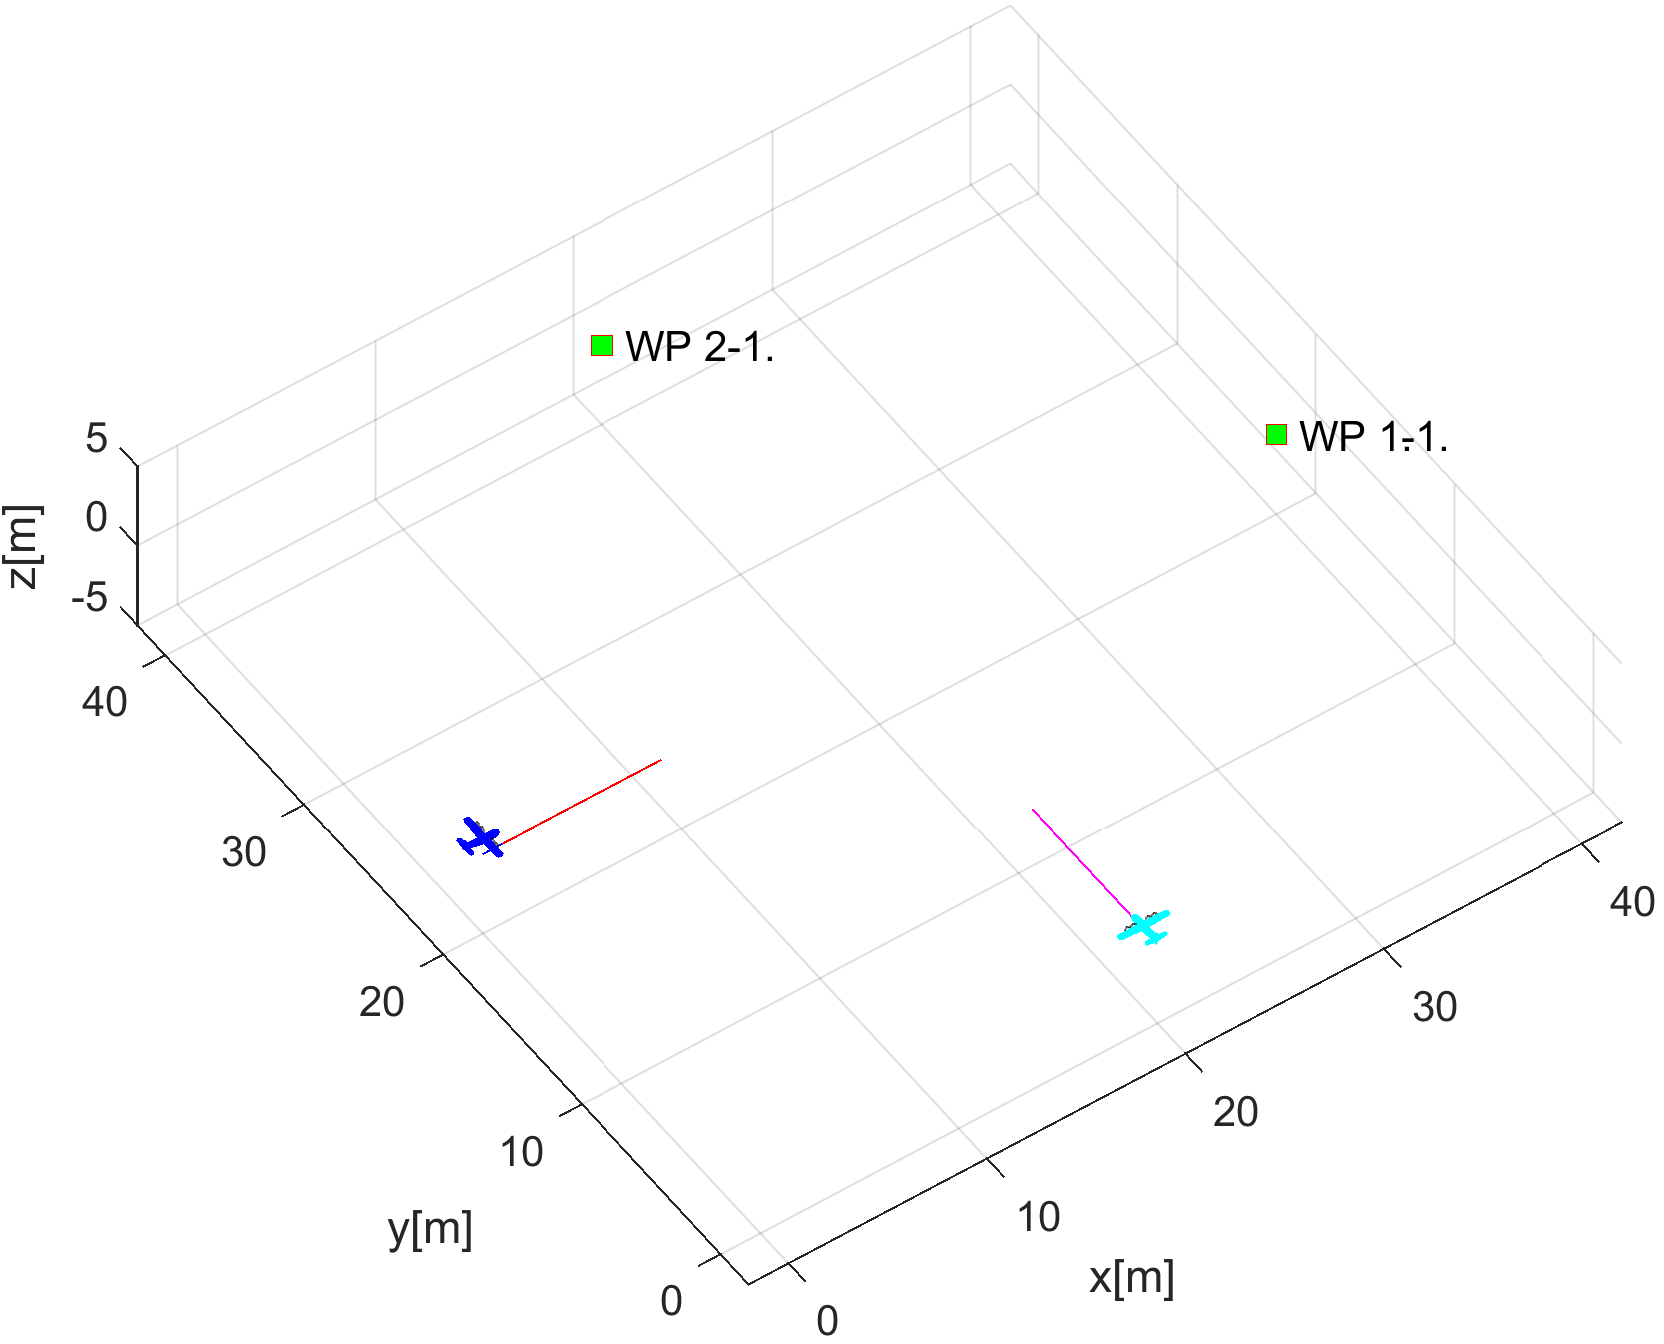
\includegraphics[width=0.9\linewidth]{\FIGDIR/NS025UtmEmergencyConverging00001}
        \caption{Situation detection.}
        \label{fig:emergencyConvergingSituationDetection}
    \end{subfigure}
    \begin{subfigure}{0.48\textwidth}
    	\centering
        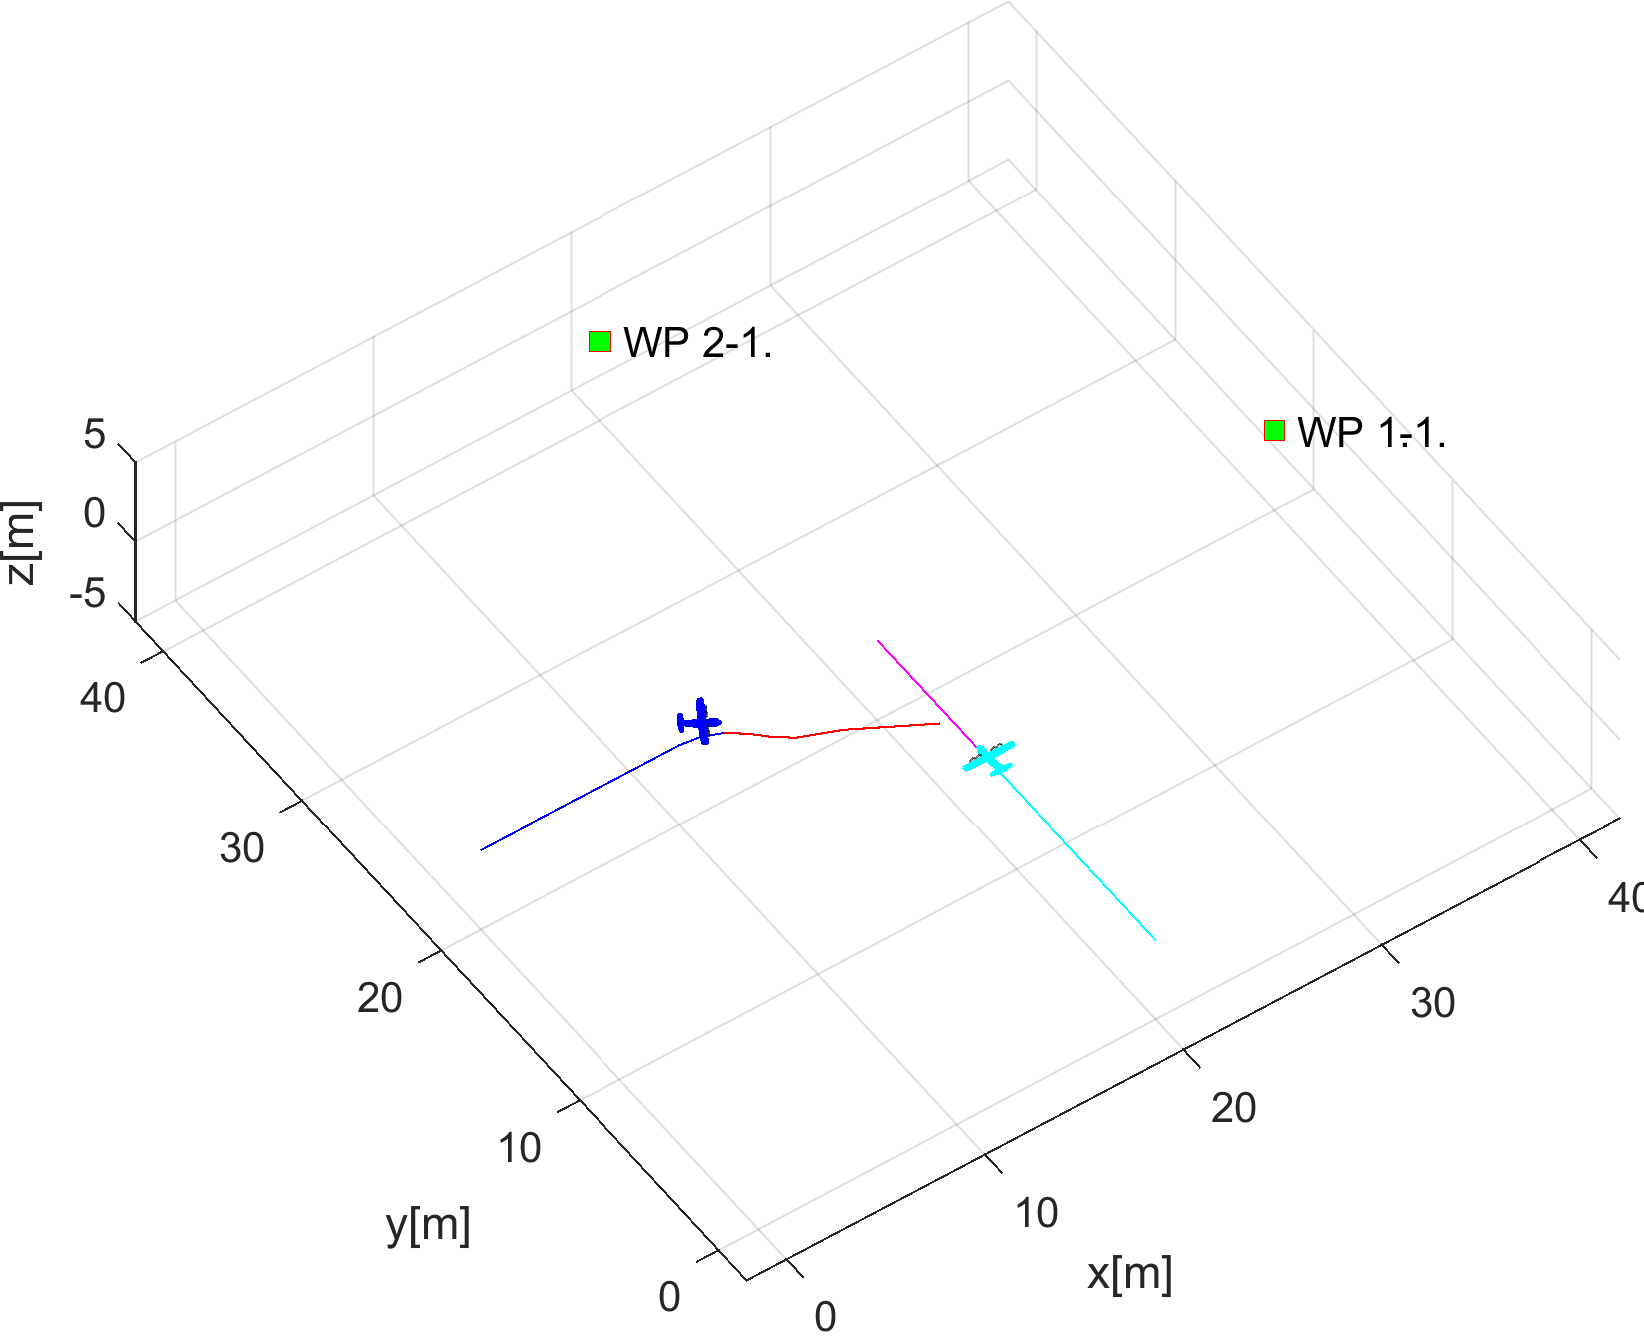
\includegraphics[width=0.9\linewidth]{\FIGDIR/NS026UtmEmergencyConverging00012} 
        \caption{Start converging.}
        \label{fig:emergencyConvergingStart}
    \end{subfigure}
    \\
    \begin{subfigure}{0.48\textwidth}
    	\centering
        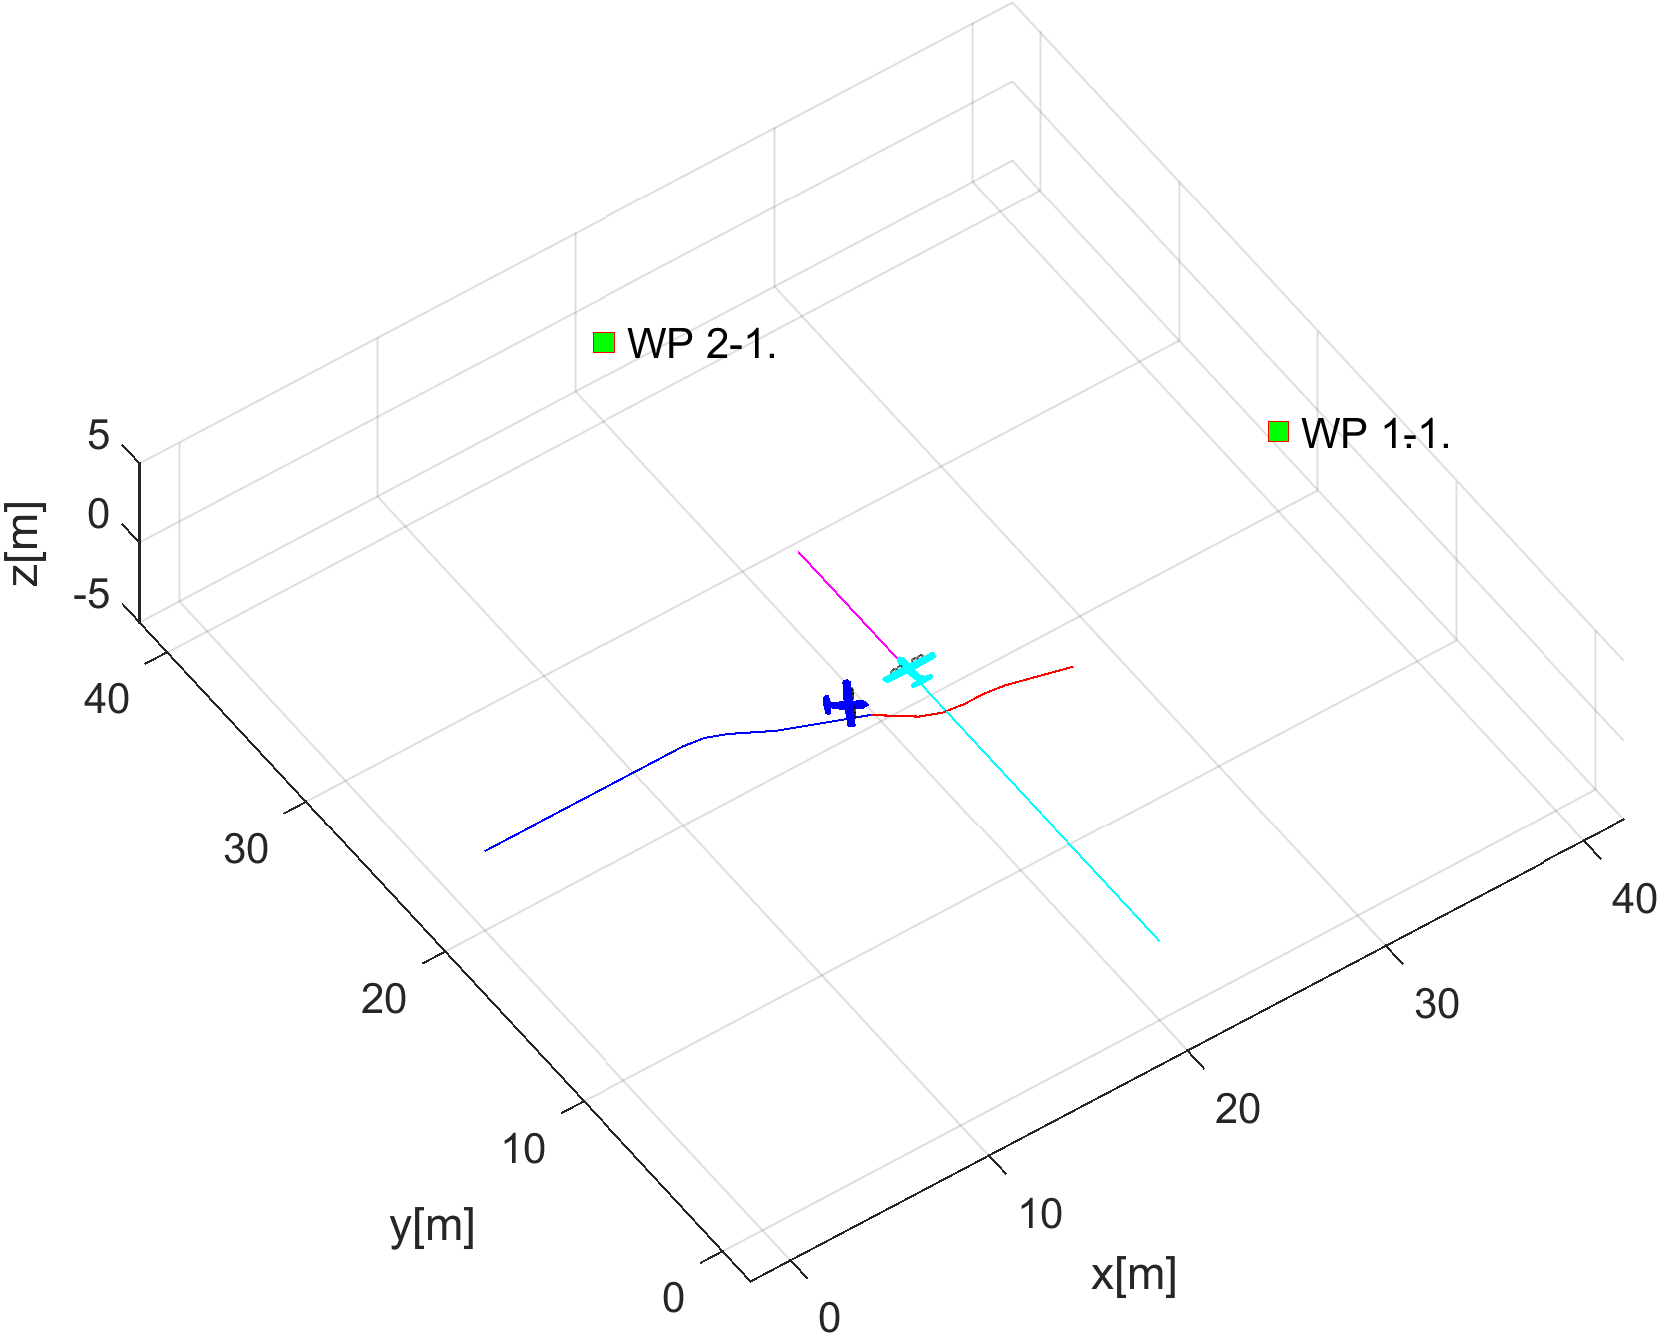
\includegraphics[width=0.9\linewidth]{\FIGDIR/NS027UtmEmergencyConverging00018} 
        \caption{Near miss case.}
        \label{fig:emergencyConvergingEnd}
    \end{subfigure}
    \begin{subfigure}{0.48\textwidth}
    	\centering
        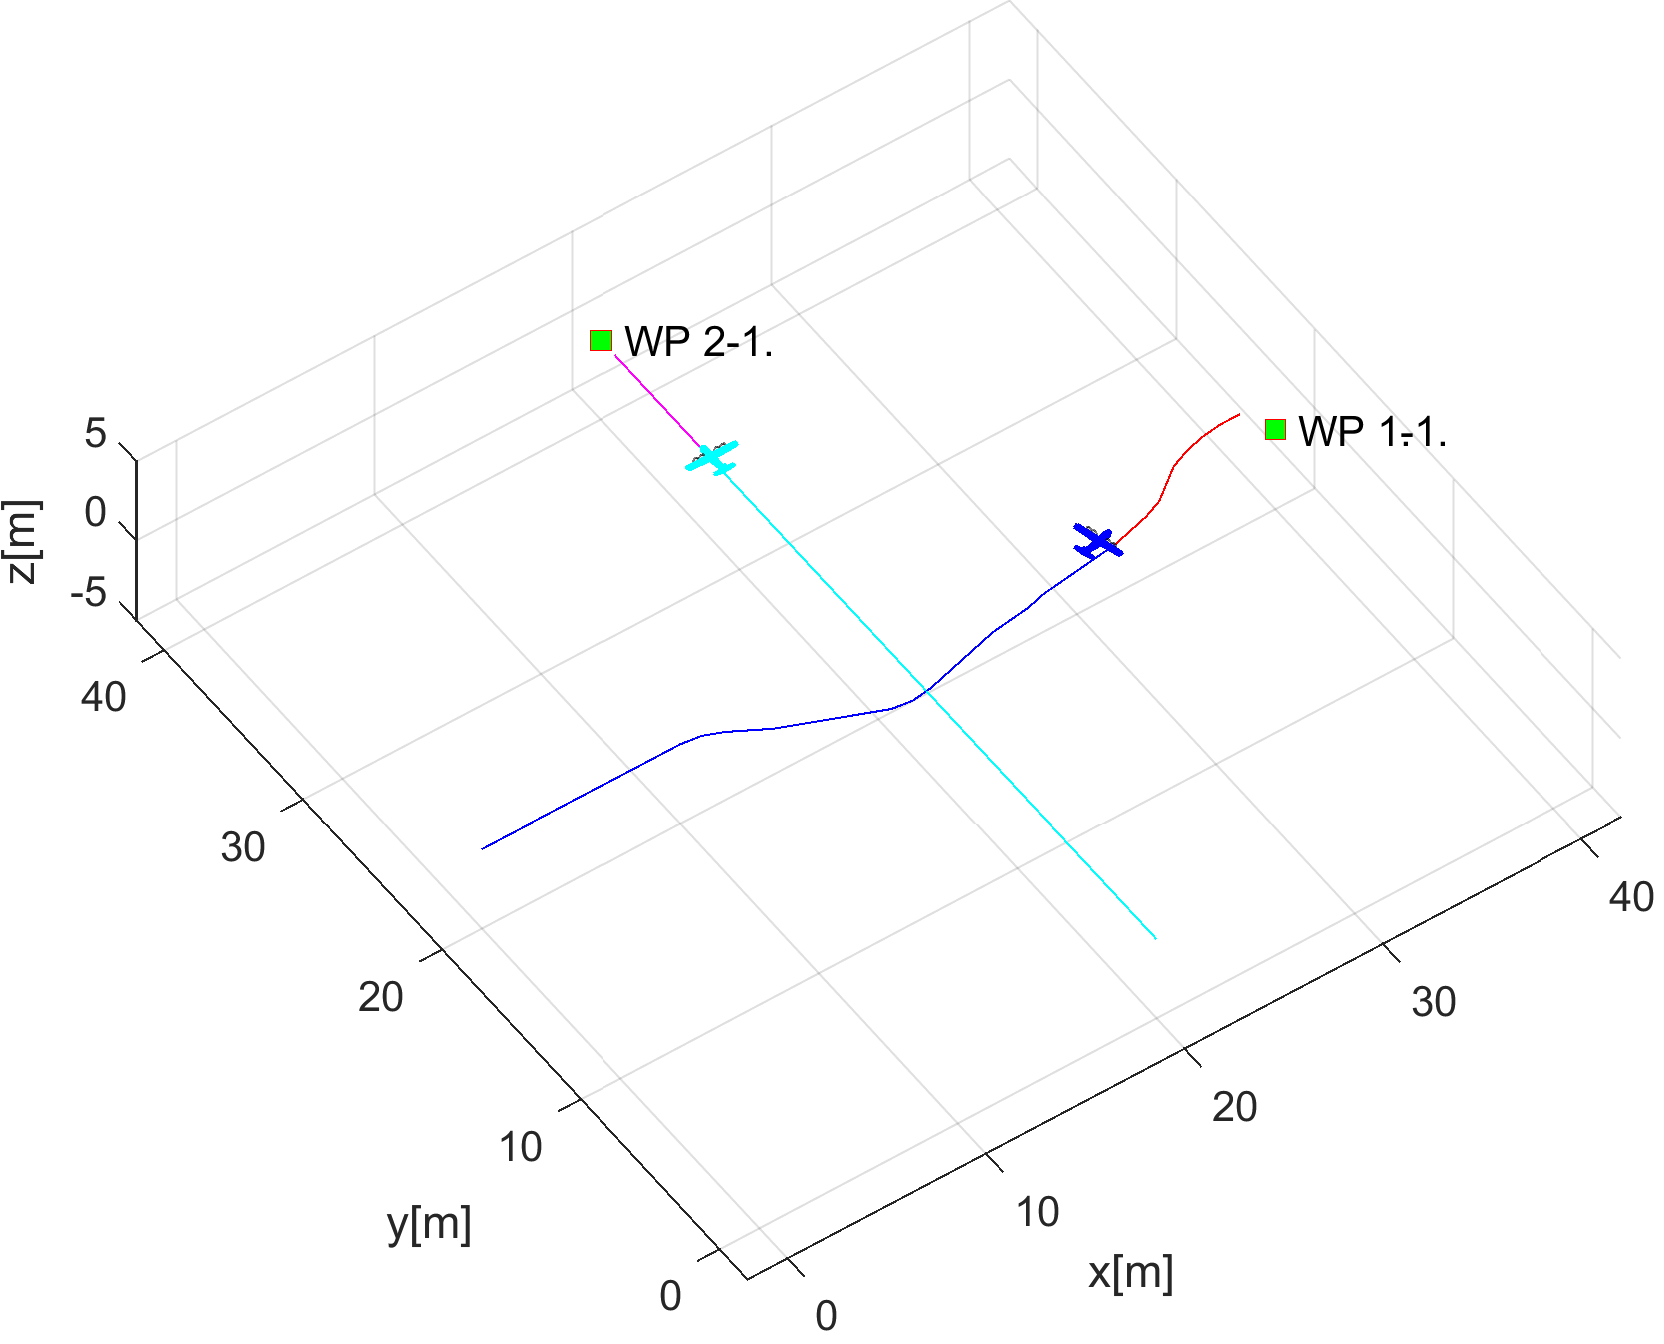
\includegraphics[width=0.9\linewidth]{\FIGDIR/NS028UtmEmergencyConverging00032} 
        \caption{Waypoints reach.}
        \label{fig:emergencyConvergingWaypointReach}
    \end{subfigure}
    \caption{Test scenario for \emph{Emergency converging} (Intruder avoidance). }
    \label{fig:testCaseEmergencyConverging}
\end{figure}

\begin{figure}[H]
    \centering
    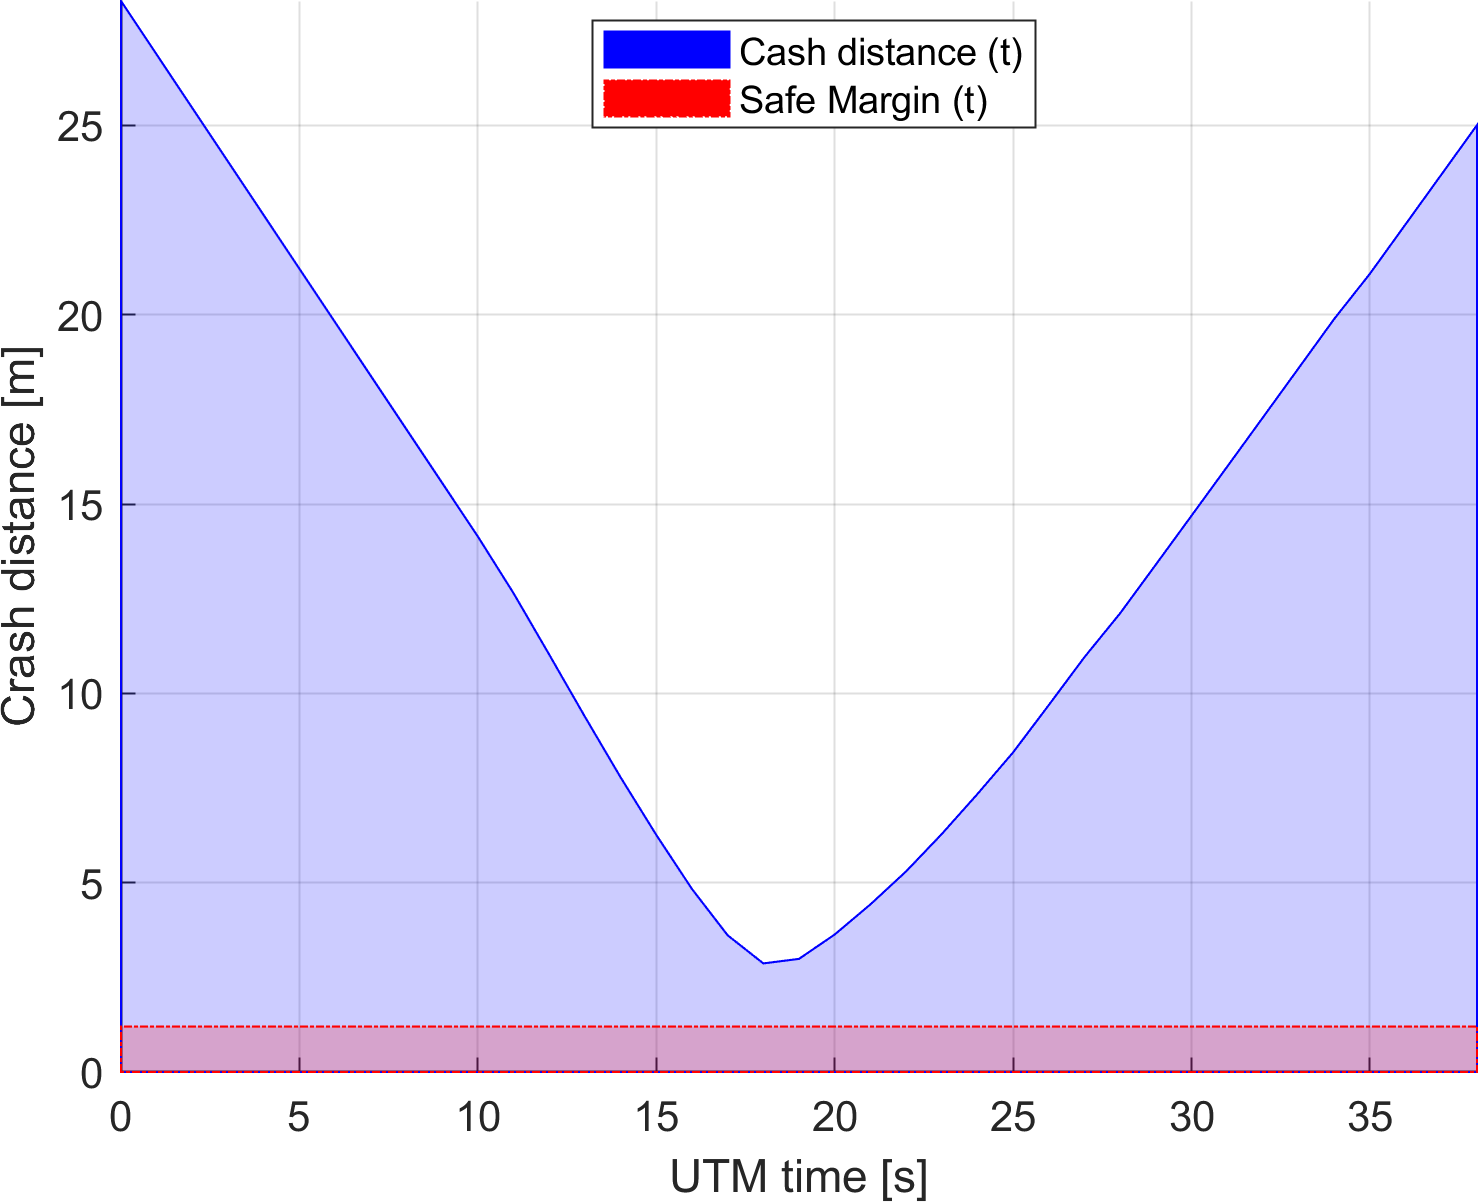
\includegraphics[width=0.55\linewidth]{\FIGDIR/NS029UtmEmergencyConvergingPerformance} 
    \caption{Distance to safety margin evolution for \emph{emergency converging scenario}.}
    \label{fig:testCaseEmergencyConvergingAvoidancePerformance}
\end{figure}

\paragraph{Distance to Safety Margin Evolution:} There is a need to compare the mutual distance between both UAS (y-axis [m]) and its evolution over UTM time (x-axis [s]). The \emph{mutual} distance of \emph{UAS 1} to \emph{UAS 2} is given by \emph{blue line}. The \emph{Safety margin} value is denoted by the red line at a  \emph{constant value} of $1.2$ $m$.

The \emph{Proper avoidance Invocation} is shown when UAS systems are getting closer to each other, and they enter (Emergency Avoidance Mode) to provide \emph{active separation}. The \emph{Mutual distance evolution} (blue line) does not cross \emph{safety margin} (red line).


\paragraph{Distance to Safety Margin Peaks:} Minimal and Maximal mutual distance to safety margin is summarized in (tab. \ref{tab:testCaseEmergencyConvergingSafetyMarginDistances}). The closest to the collision are UAS systems when the distance to safety margin is $1.6676m$.

The \emph{minimal distance to safety margin  $\ge$ 0} which means that the \emph{safety acceptance criterion} is fulfilled. 

\begin{table}[H]
    \centering
    \begin{tabular}{c|c||c}
    \multicolumn{2}{c||}{UAS:} & 1-2 \\\hline\hline
    \multirow{2}{*}{Distance to Safety Margin} & min & 1.6676 \\\cline{2-3}
                                            & max & 27.0843 \\
    \end{tabular}
    \caption{Distance to safety margin peaks for the \emph{emergency converging scenario}.}
    \label{tab:testCaseEmergencyConvergingSafetyMarginDistances}
\end{table}

\paragraph{Path Tracking Performance:} All waypoints (green numbered squares) for both  UAS have been reached (fig. \ref{fig:emergencyConvergingTrajectoryTrackingPerformance}). \emph{Reference trajectories} (green dashed lines), between the initial position (green square marked S) and goal waypoint (green square marked 1) are split into three XYZ values with respective figures. The tracked value is on y-axis [m] and time on x-axis [s]. The blue lines represent real parameter evolution over time.

Following observations can be made from path tracking (fig. \ref{fig:emergencyConvergingTrajectoryTrackingPerformance}) and preferred separations (tab. \ref{tab:aboidanceParametersForEmergencyConvergingScenario}):

\begin{enumerate}
    \item UAS 1 (fig. \ref{fig:emergencyConvergingUAS1PathTracking}) is using \emph{horizontal separation} (y-axis). The UAS diverges from the reference trajectory to minimum necessary time.
    
    \item UAS 2 (fig. \ref{fig:emergencyCovnergingUAS2PathTracking}) has the right of way and is not using any active avoidance mechanism. 
\end{enumerate}

\begin{figure}[H]
    \centering
    \begin{subfigure}{0.48\textwidth}
    	\centering
        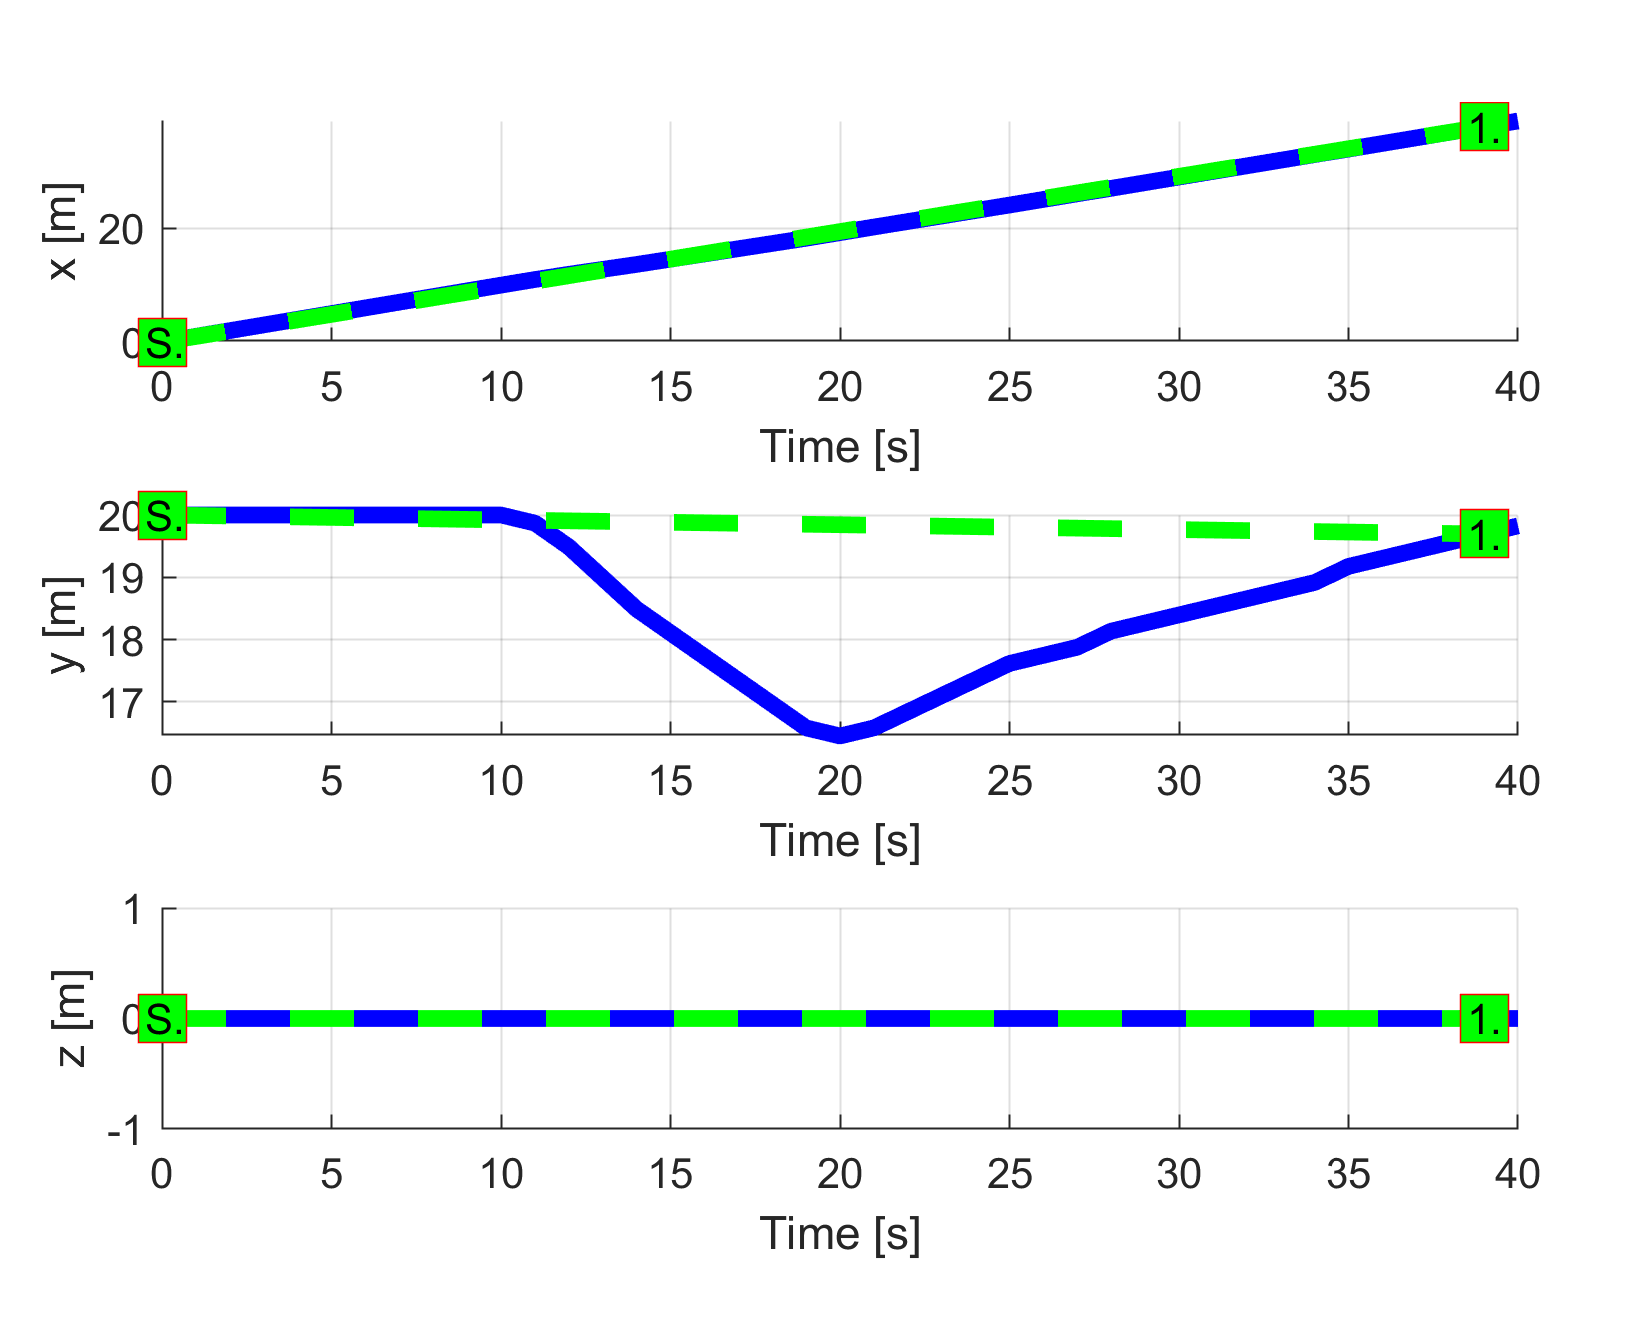
\includegraphics[width=0.9\linewidth]{\FIGDIR/NS030UtmEmergencyConvergingUAV1PathFollowing}
        \caption{UAS 1.}
        \label{fig:emergencyConvergingUAS1PathTracking}
    \end{subfigure}
    \begin{subfigure}{0.48\textwidth}
	    \centering
        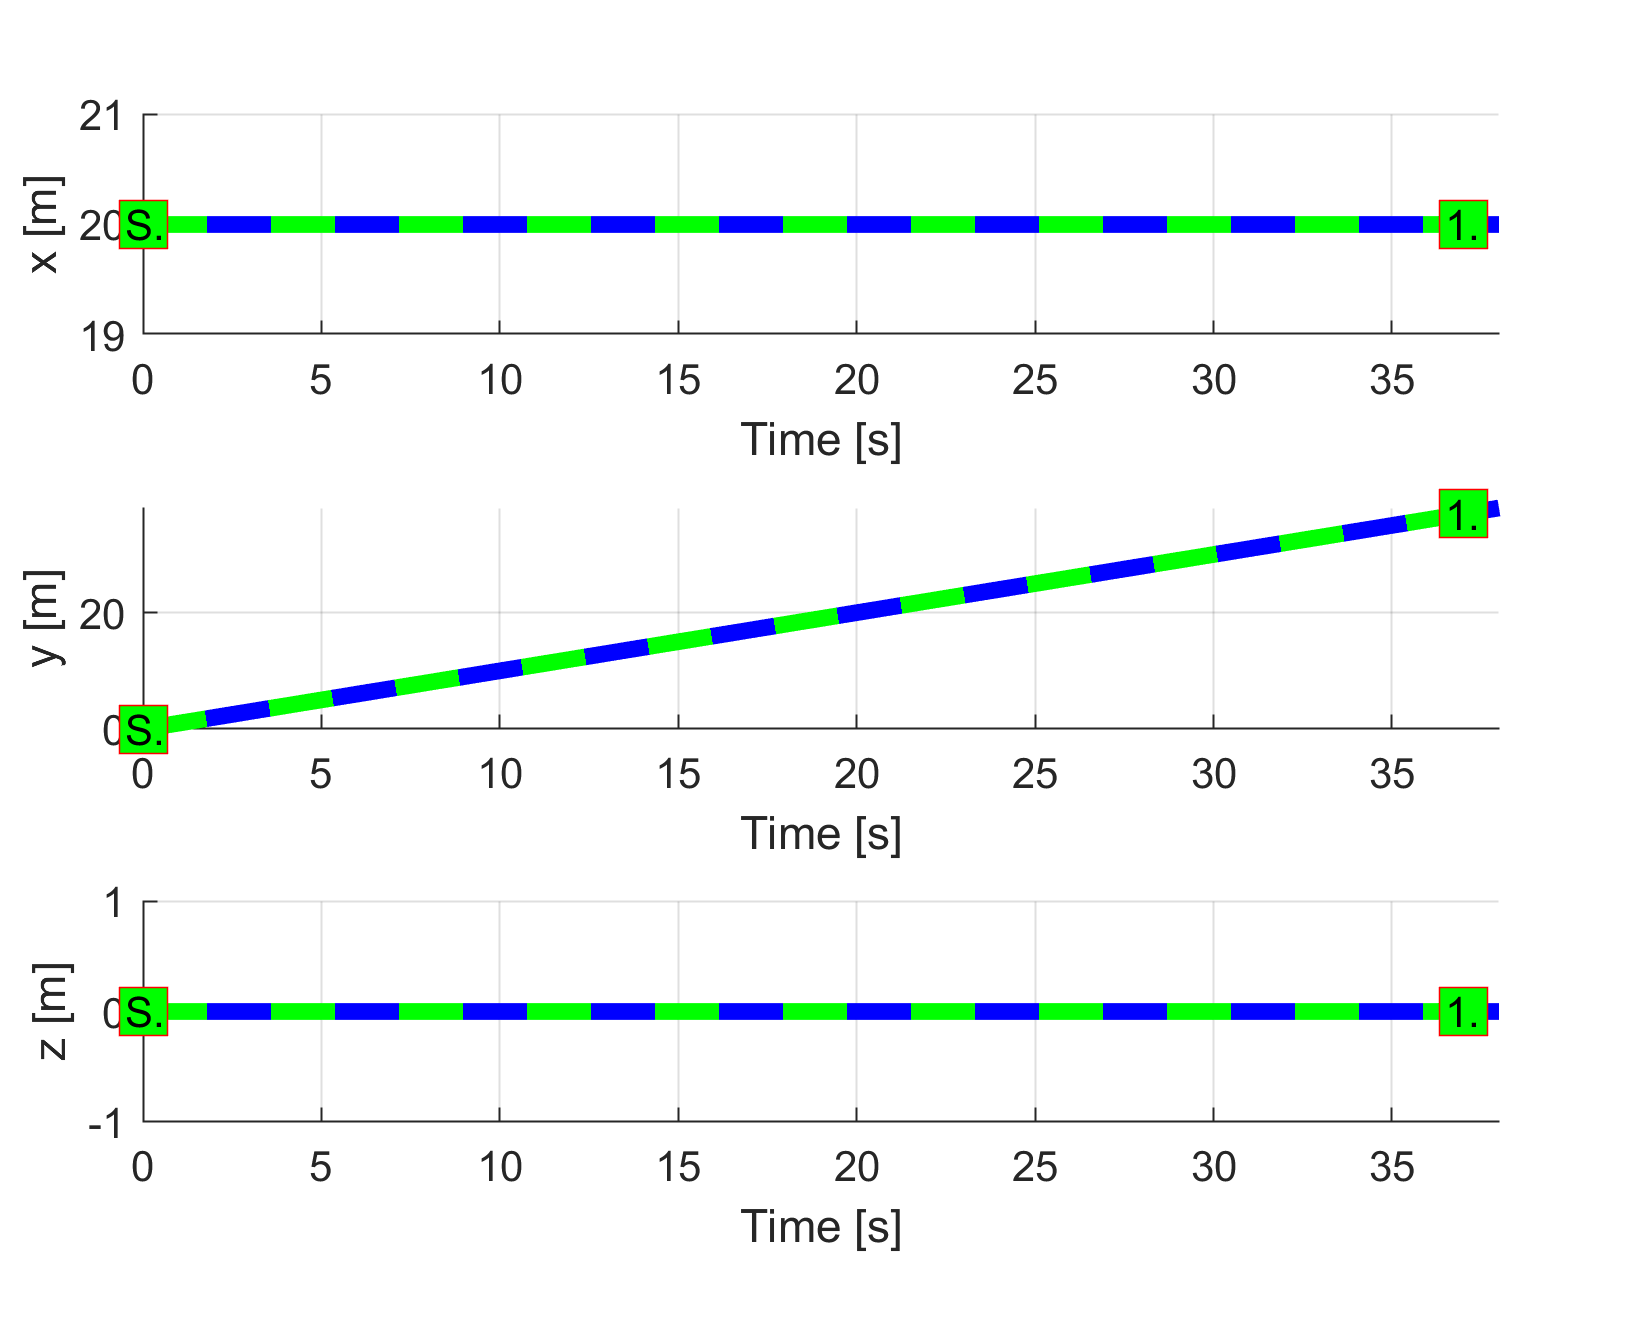
\includegraphics[width=0.9\linewidth]{\FIGDIR/NS031UtmEmergencyConvergingUAV2PathFollowing} 
        \caption{UAS 2.}
        \label{fig:emergencyCovnergingUAS2PathTracking}
    \end{subfigure}
    \caption{\emph{Trajectory tracking} for \emph{Emergency converging} test case. }
    \label{fig:emergencyConvergingTrajectoryTrackingPerformance}
\end{figure}

\paragraph{Path Following Deviations:} \emph{Deviations} (tab. \ref{tab:pathTrackingParametersForEmergencyConverging}) are in expected ranges considering the  \emph{mission plans} (tab. \ref{tab:missionSetupEmergencyConvergingScenario}) and \emph{separation safety margin} (tab. \ref{tab:aboidanceParametersForEmergencyConvergingScenario}).
    
\begin{table}[H]
    \centering
    \begin{tabular}{c||c|c}
        \multirow{2}{*}{Param.} & UAS 1     & UAS 2\\\cline{2-3}
                        & $\mathscr{WP}_1$  & $\mathscr{WP}_1$\\\hline\hline
          $\max |x|$    & 0                 & 0 \\\hline
          $\max |y|$    & 3.25              & 0 \\\hline
          $\max |z|$    & 0                 & 0 \\\hline
          $\max dist.$  & 3.25              & 0 \\
    \end{tabular}
    \caption{Path tracking properties for the\emph{Emergency converging} scenario.}
    \label{tab:pathTrackingParametersForEmergencyConverging}
\end{table}

% 05 Emergency Converging
\paragraph{Computation Load:} The \emph{computation load} for \emph{scenario} (fig.\ref{fig:emergencyConvergingComputationTime}) shows used time (y-axis) over decision frame (x-axis).

The \emph{computation time} is increased only for UAS 1 during the avoidance period. The UAS 2 remains unaffected because it has the right of way.

\begin{figure}[H]
    \centering
    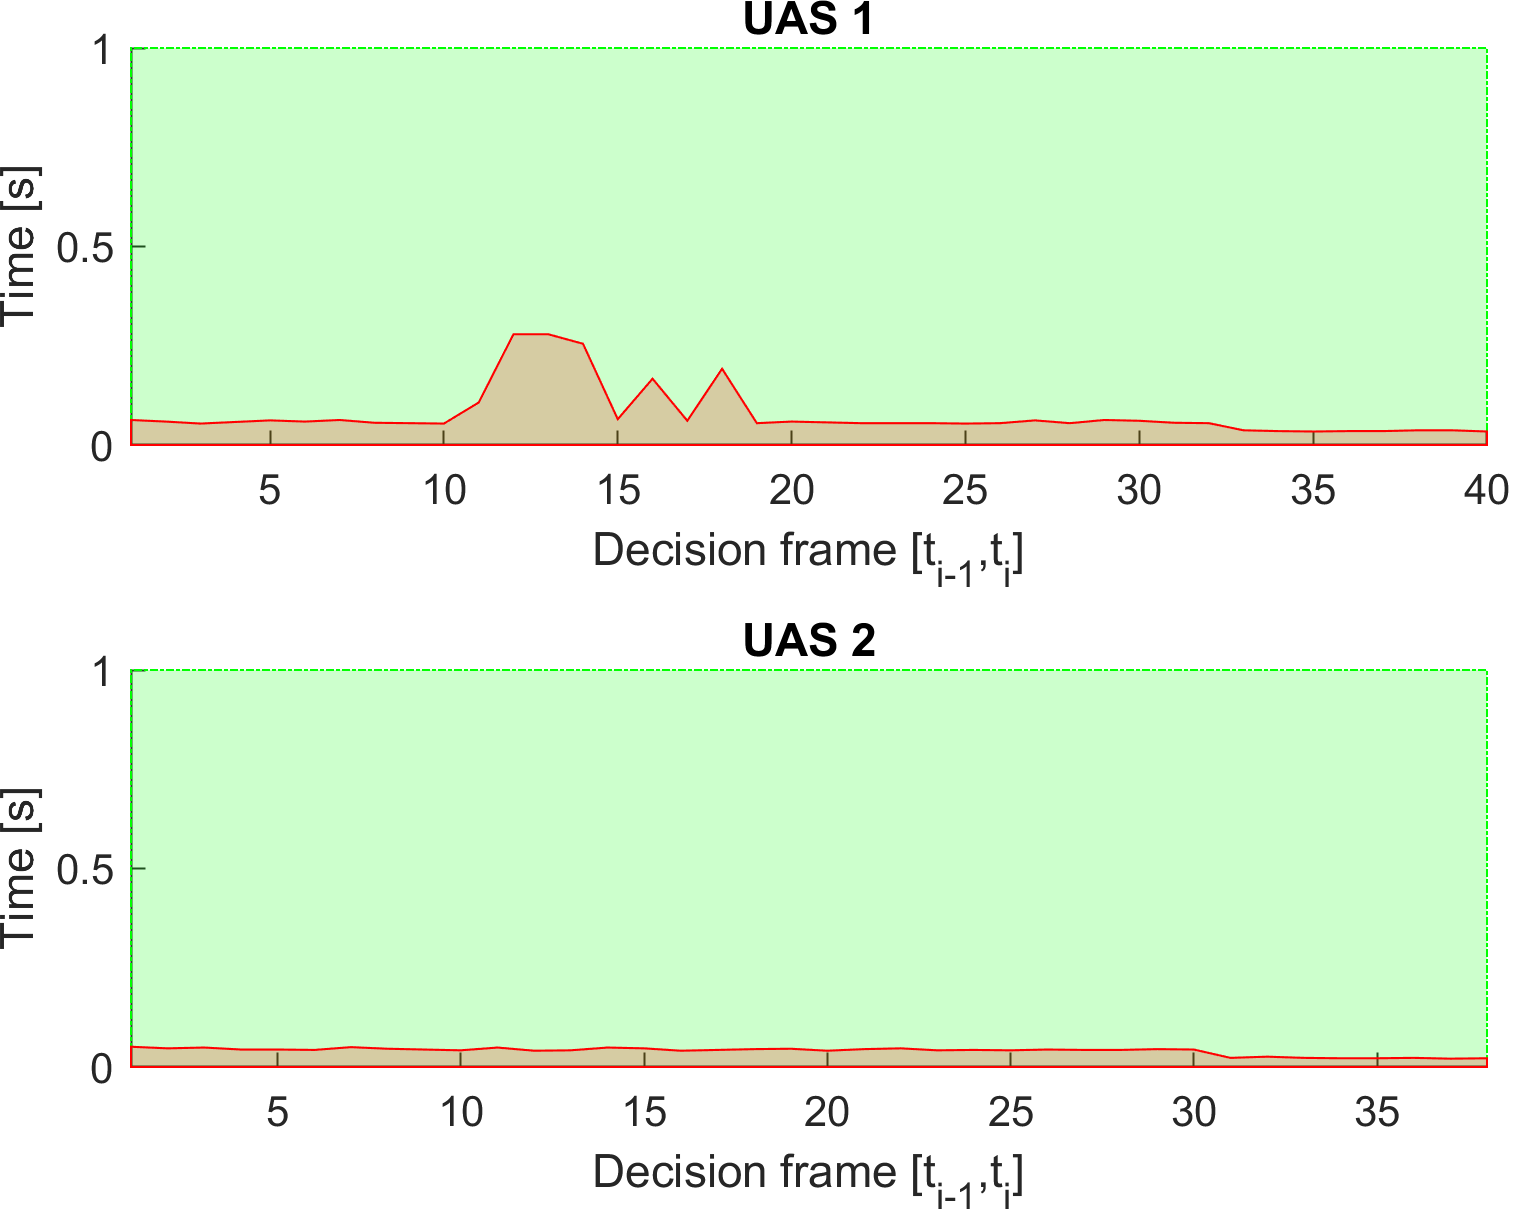
\includegraphics[width=0.65\linewidth]{\FIGDIR/NS096EmergencyConvergingComputationTime} 
    \caption{Computation time for \emph{Emergency converging} scenario.}
    \label{fig:emergencyConvergingComputationTime}
\end{figure}


    	\subsection{Emergency Head on}\label{s:testEmergencyHeadOn}

\paragraph{Scenario:} Two  \emph{UAS} systems are flying in an \emph{uncontrolled airspace} (altitude $\le$ 500 ft. Above the Ground Level) with missions defined in (tab. \ref{tab:missionSetupEmergencyHeadOnScenario}). Both \emph{UAS} are in the  \emph{Navigation mode} with active \emph{ADSB-In/Out}, receiving position notifications from each other. Cruising altitude is sufficient for horizontal separation (50-100 ft. Above Ground Level). \emph{Horizontal separation} is preferred mode for both \emph{UAS}.


\begin{table}[H]
    \centering
    \begin{tabular}{c||c|c||c}
        \multirow{2}{*}{UAS} &\multicolumn{2}{c||}{Position} & \multirow{2}{*}{$\mathscr{WP}_1$} \\\cline{2-3}
          & $[x,y,z]$           & $[\theta,\varpi,\psi]$           & \\\hline\hline
        1 & $[0,20,0]^T $       & $[0^\circ,0^\circ,0^\circ]^T$    & $[40,20,0]^T$\\\hline 
        2 & $[40,20,0]^T $       & $[0^\circ,0^\circ,180^\circ]^T$  & $[0,20,0]^T$\\ 
    \end{tabular}
    \caption{Mission setup for \emph{Emergency head on} scenario.}
    \label{tab:missionSetupEmergencyHeadOnScenario}
\end{table}


\begin{note}
\emph{Collision point} is expected at $\mathscr{C}=[20,20,0]^T$. The \emph{angle of approach} is $180^{\circ}$  which classifies situation as \emph{Head on maneuver} (fig. \ref{fig:HeadOnApproachTheoretical}).
\end{note}


\paragraph{Main Goal:} Show two \emph{non-cooperative } UAS avoidance for \emph{Head-on approach scenario} in \emph{uncontrolled} airspace.


\paragraph{Acceptance criteria:} 
\begin{enumerate}
    \item\emph{Proper mode invocation} - when an intruder intersects the opposing \emph{UAS} Navigation grid, bot intruder and \emph{UAS} will switch to \emph{Emergency Avoidance Mode}. None of the \emph{UAS} have \emph{Right Of the Way}.
    
    \item\emph{Minimal Safety Margin distance} $\ge 0m$. That means the mutual distance of both \emph{UAS centers} does not go below given \emph{safety margin}.
    
    \item\emph{Both UAS} will reach own goal waypoint (tab. \ref{tab:missionSetupEmergencyHeadOnScenario}).

\end{enumerate}

\paragraph{Testing setup:} The \emph{standard test setup} for each UAS defined in (tab \ref{tab:testMovementOrientations}, \ref{tab:testUASBasicParameters}, \ref{tab:testNavigationGridBasic}, \ref{tab:testAvoidanceGridBasic}, \ref{tab:testUASColoring}) is used with following without parameter override.

\emph{Intruder intersection} model has been chosen depending on UAS (tab. \ref{tab:aboidanceParametersForEmergencyHeadOnScenario}). Each UAS is equipped with \emph{ADS-B In/Out} sensor obtaining/distributing following information:

\begin{enumerate}
    \item \emph{Position} - in operational section coordinate frame.
    
    \item \emph{Velocity} - vector representation in given coordinate frame.
    
    \item \emph{Class size} - class body radius based on UAS propulsion and size.
    
    \item \emph{Safety margin set} - set of safety margins for different collision cases.
\end{enumerate}

\noindent \emph{Avoidance parameters} for \emph{Emergency head-on scenario} are given in (tab. \ref{tab:aboidanceParametersForEmergencyHeadOnScenario}). Each UAS has same speed set to $1 m s^{-1}$. None of them have the \emph{Right of The Way}. 

\emph{Safety margin} is considered as sum of both participants \emph{near miss margins}. In this case default safety margin is considered as $1.2$ $m$.

\begin{table}[H]
    \centering
    \begin{tabular}{c||c|c|c||c|c||c}
        \multirow{2}{*}{UAS} & \multicolumn{3}{c||}{Parameters} & \multicolumn{2}{c||}{Margins} & \multirow{2}{*}{Separation}                                            \\\cline{2-6}
                             & velocity & intruder model & ROW        & body & safety \\\hline\hline
        1                    & 1        & body (timed)  & false            & 0.3         & 0.6           & horizontal\\\hline
        2                    & 1        & body (timed)  & false             & 0.3         & 0.6  & horizontal          \\
    \end{tabular}
    \caption{Avoidance parameters for  \emph{Emergency head on} scenario.}
    \label{tab:aboidanceParametersForEmergencyHeadOnScenario}
\end{table}


\begin{note}
Both UAS are using  body (sec. \ref{s:bodyvolumeIntersection}) intersection model, reflecting both body volume along expected trajectory. Both UAS have preference for \emph{horizontal} separation mode, typical for planes.
\end{note}

\paragraph{Simulation Run:} Notable moments from the simulation run (fig. \ref{fig:testCaseEmergencyHeadOnApproach}) are following:

\begin{enumerate}
    \item \emph{Situation detection} (fig. \ref{fig:emergencyConvergingSituationDetection}) - UAS 1 (blue)  is approaching UAS 2 (cyan) with $130^\circ \le angle Of Approach \le 180^\circ$, this is considered head on approach. Head on approach  give the \emph{right of the way} neither to \emph{UAS 1} nor \emph{UAS 2}. \emph{Intruder intersection model} for opposite UAS is created in respective \emph{avoidance grids}. \emph{Head on emergency avoidance} starts independently in each UAS without intruders coordination. First \emph{avoidance maneuver} is invoked when the \emph{intruder intersection model} constraints any trajectory in the \emph{avoidance grid}. When this happens \emph{Navigation mode} switch to the \emph{Emergency avoidance mode}.
                
    \item \emph{Before near miss} (fig. \ref{fig:emergencyHeadOnBeforeNearMiss}) - both \emph{UAS} are in \emph{emergency avoidance mode}, sticking to right side avoidance maneuver.
    
    \item \emph{Near miss case} (fig. \ref{fig:emergencyHeadOnNearMiss}) - UAS 1 to UAS 2 closest distance. The safety margin for \emph{near miss} has not been breached. The safety margin for \emph{well clear} in uncontrolled airspace is invalid. Both UAS are using also \emph{Horizontal separation} to avoid each other, \emph{Emergency avoidance mode} is switched to the \emph{Navigation mode} when risk of an \emph{aerial clash} is voided.
    
    \item \emph{After near miss} (fig. \ref{fig:emergencyHeadOnAfterNearMiss}) - both \emph{UAS} are tracking back to respective waypoint, correcting \emph{altitude} (Z-axis in (fig. \ref{fig:emergencyHeadOnTrajectoryTrackingPerformance})) first.
    
    \item Note \emph{Collision point} was expected at $\mathscr{C}=[20,20,0]^T$
    
    \item Note \emph{Both UAS} used \emph{horizontal} (primary), \emph{vertical} (secondary) separation (fig \ref{fig:emergencyHeadOnTrajectoryTrackingPerformance}).
    
    \item Note \emph{Both UAS} decision times were \emph{synchronized}, this is not an assumption, but it shows critical performance. Usually safety margin is bloated for (eq.\ref{safetyMarginBloat}).
\end{enumerate}


\begin{figure}[H]
    \centering
    \begin{subfigure}{0.75\textwidth}
        \centering
        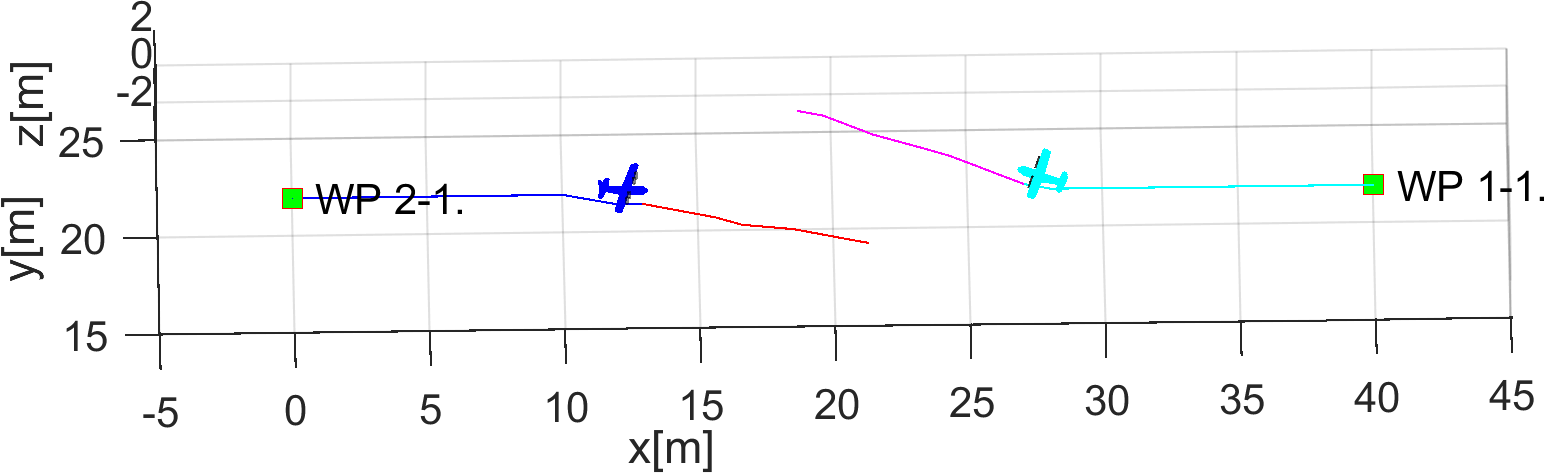
\includegraphics[width=0.9\linewidth]{\FIGDIR/NS032UtmEmergencyHeadOn00013}
        \caption{Situation detection.}
        \label{fig:emergencyHeadOnSituationDetection}
    \end{subfigure}
    \\
    \begin{subfigure}{0.75\textwidth}
        \centering
        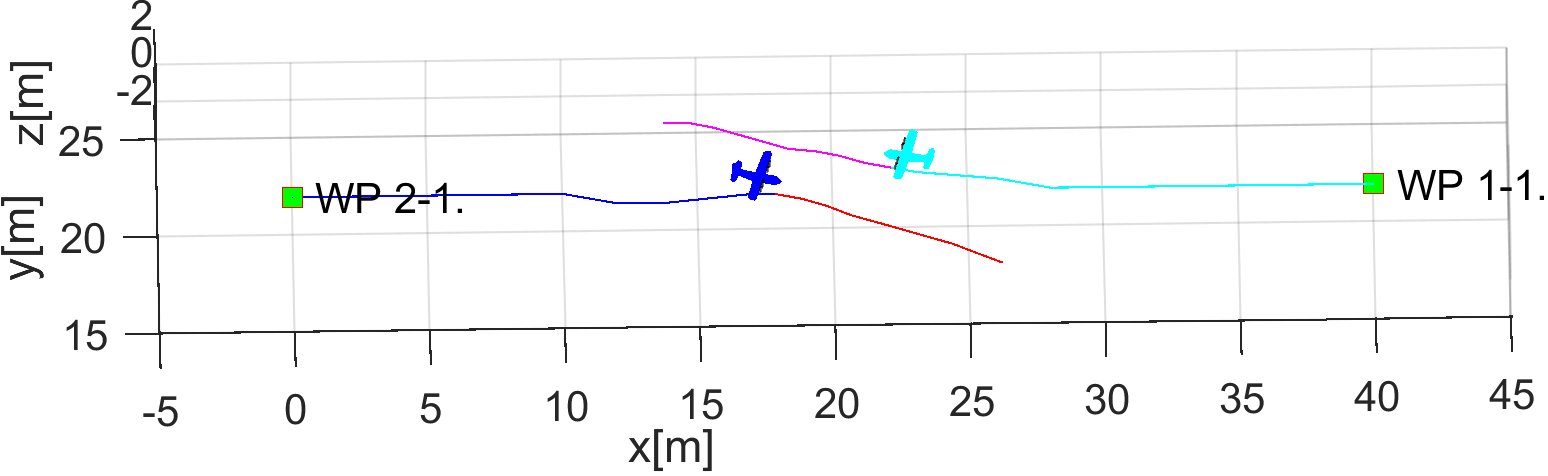
\includegraphics[width=0.9\linewidth]{\FIGDIR/NS033UtmEmergencyHeadOn00018} 
        \caption{Before near miss.}
        \label{fig:emergencyHeadOnBeforeNearMiss}
    \end{subfigure}
    \\
    \begin{subfigure}{0.75\textwidth}
        \centering
        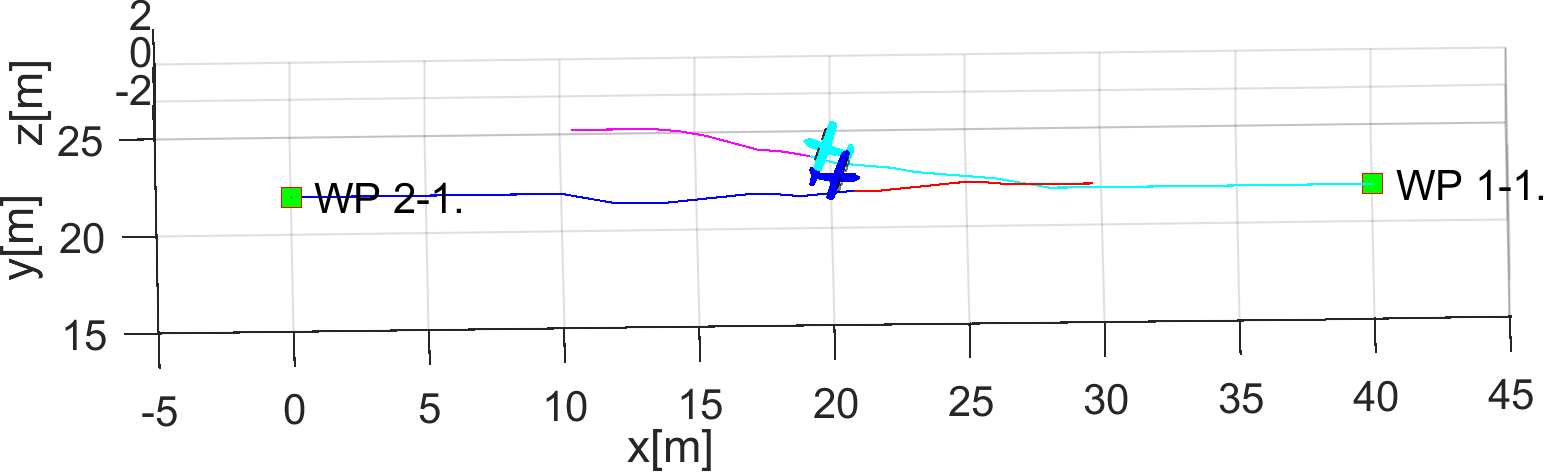
\includegraphics[width=0.9\linewidth]{\FIGDIR/NS034UtmEmergencyHeadOn00021} 
        \caption{Near miss.}
        \label{fig:emergencyHeadOnNearMiss}
    \end{subfigure}
    \\
    \begin{subfigure}{0.75\textwidth}
        \centering
        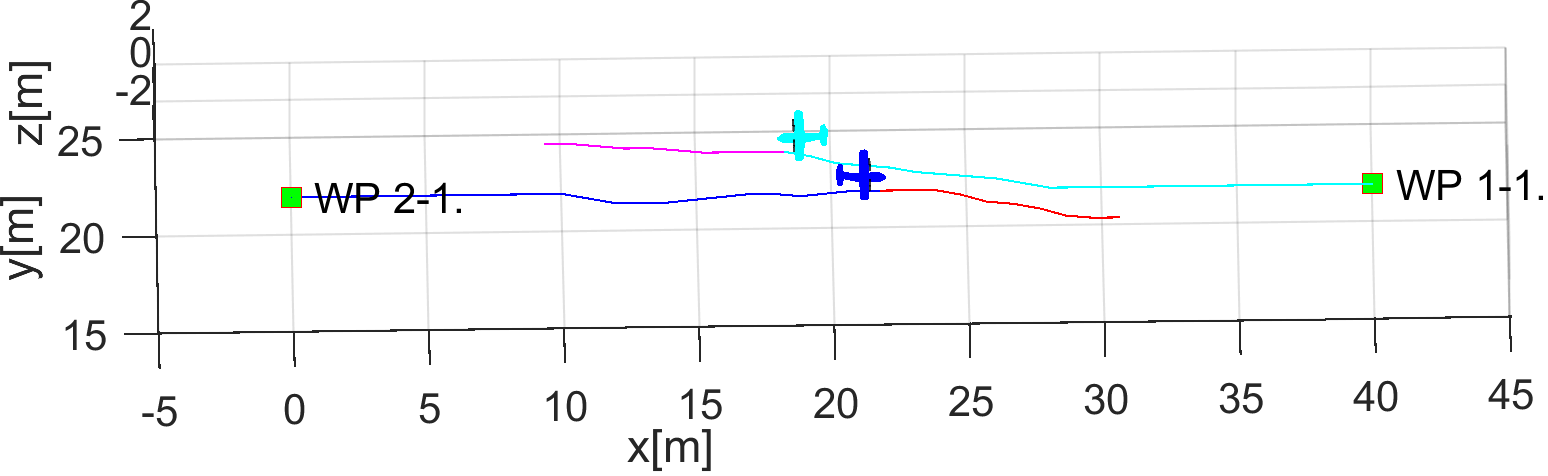
\includegraphics[width=0.9\linewidth]{\FIGDIR/NS035UtmEmergencyHeadOn00022} 
        \caption{After near miss.}
        \label{fig:emergencyHeadOnAfterNearMiss}
    \end{subfigure}
    \caption{Test scenario for \emph{Emergency head on approach} (Intruder avoidance). }
    \label{fig:testCaseEmergencyHeadOnApproach}
\end{figure}


\paragraph{Distance to Safety Margin Evolution:} There is need to compare mutual distance between both UAS (y-axis [m]) and its evolution over synchronized \emph{UTM time} (x-axis [s].) The \emph{mutual distance} between bodies of \emph{UAS 1}, \emph{UAS 2} (blue line) compared to \emph{Safety Margin} (red line) is given in (fig. \ref{fig:testCaseHeadOnAvoidancePerformance}). The \emph{Safety Margin} value was constant for all time at value $1.2$ $m$ which is double of \emph{Near Miss Margin for UAS 1 UAS 2}.

The proper \emph{Avoidance Invocation} is shown when \emph{UAS} systems are getting closer to each other and they starts their \emph{separation phase} (Emergency Avoidance Mode switch). The mutual distance (blue line) does not cross \emph{safety margin} (red line).

\begin{figure}[H]
    \centering
    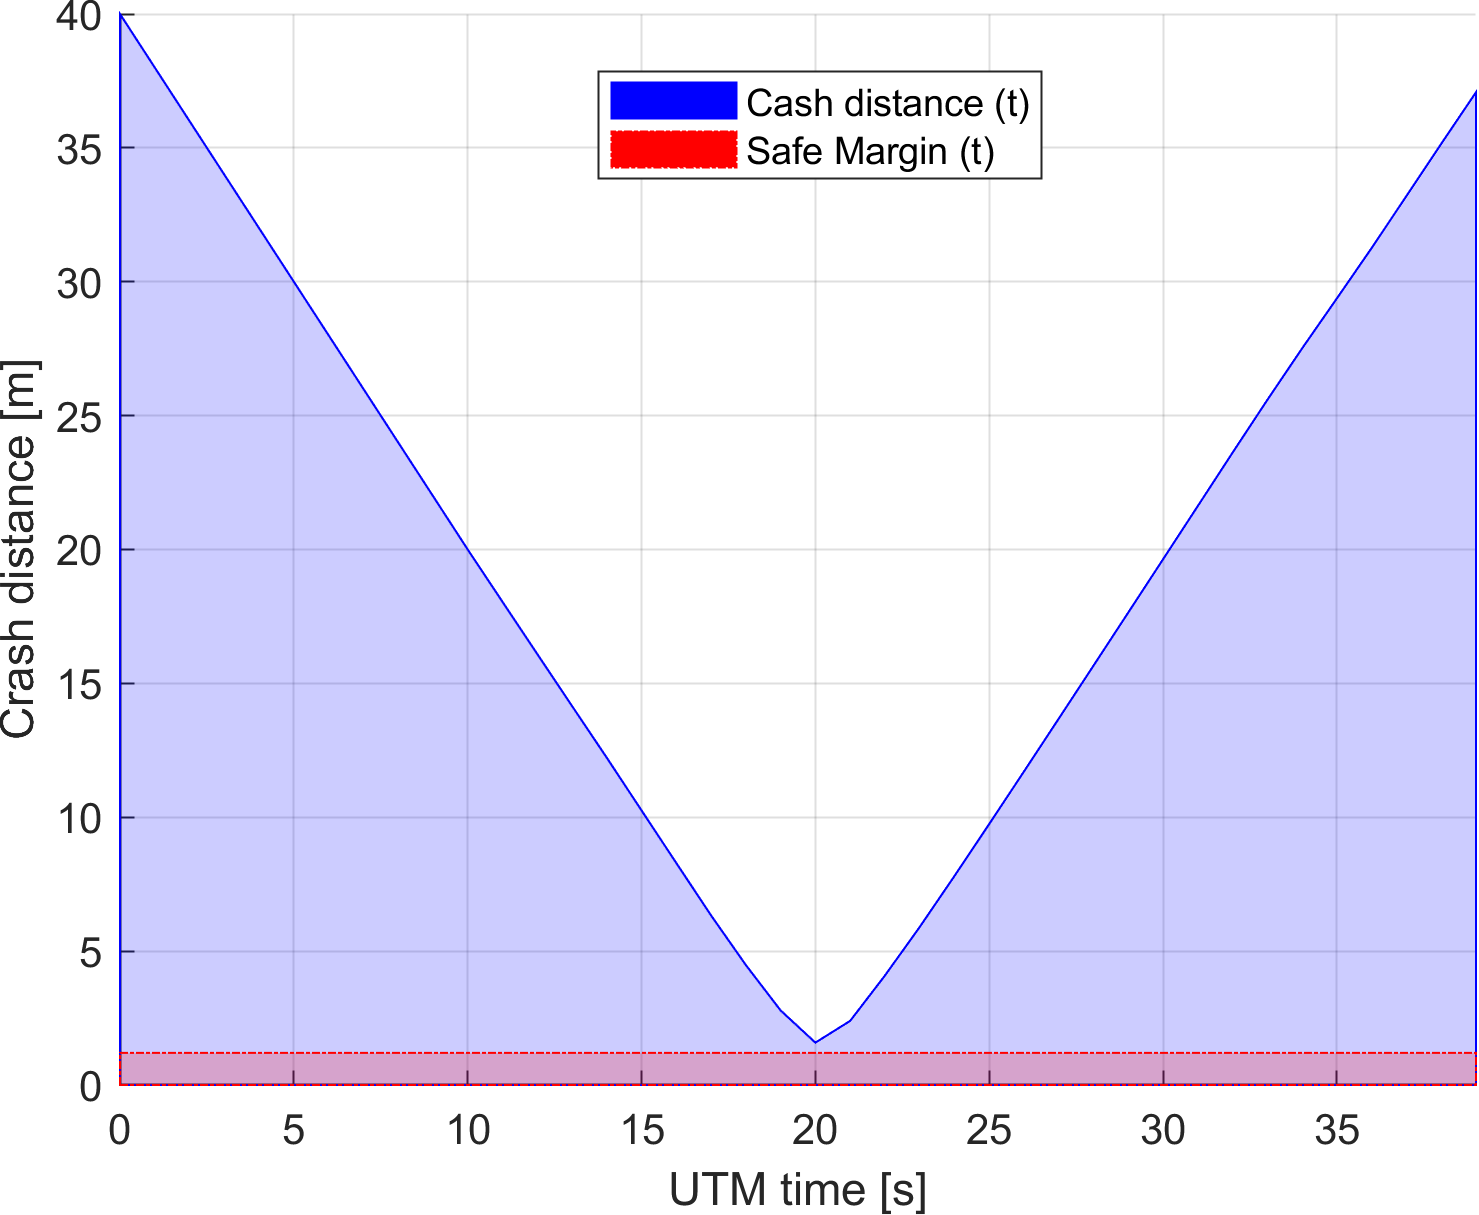
\includegraphics[width=0.55\linewidth]{\FIGDIR/NS036UtmEmergencyHeadOnPerformance} 
    \caption{Distance to safety margin evolution for \emph{emergency head on scenario}.}
    \label{fig:testCaseHeadOnAvoidancePerformance}
\end{figure}


\paragraph{Distance to Safety Margin Peaks:} Minimal and Maximal mutual distance to safety margin is summarized in (tab. \ref{tab:testCaseEmergencyHeadOnSafetyMarginDistances}). The closest to collision are UAS systems  when \emph{distance to safety margin} is $0.3824 m$.

The \emph{minimal distance to safety margin} $\ge$ $0$ which means that the \emph{safety acceptance criterion} is full filled.


\begin{table}[H]
    \centering
    \begin{tabular}{c|c||c}
    \multicolumn{2}{c||}{UAS:} & 1-2 \\\hline\hline
    \multirow{2}{*}{safety margin distance} & min & 0.3824 \\\cline{2-3}
                                            & max & 38.8000 \\
    \end{tabular}
    \caption{Distance to safety margin peaks for \emph{Emergency head on scenario}.}
    \label{tab:testCaseEmergencyHeadOnSafetyMarginDistances}
\end{table}

\paragraph{Path Tracking Performance} All waypoints (green numbered squares) for both UAS have been reached (fig. \ref{fig:emergencyHeadOnTrajectoryTrackingPerformance}). \emph{Reference trajectories} (green dashed lines), between initial position (green square marked S) and goal waypoint (green square marked 1) are split into three XYZ values with respective figures. The tracked value is on y-axis [m] and time on x-axis [s]. The blue lines represents real parameter evolution over time.

Following observations can be made from path tracking (fig.\ref{fig:emergencyHeadOnTrajectoryTrackingPerformance}) and preferred separations (tab. \ref{tab:aboidanceParametersForEmergencyHeadOnScenario}):

\begin{enumerate}
    \item UAS 1 (fig. \ref{fig:emergencyHeadOnUAS1PathTracking}) is using horizontal separation going to the right (y-axis) and a little bit up (z-axis).
    
    \item UAS 2 (fig. \ref{fig:emergencyHeadOnUAS2PathTracking}) is using horizontal separation going to the right (left in GCS, y-axis) and little bit up (z-axis).
\end{enumerate}

\begin{figure}[H]
	\centering
    \begin{subfigure}{0.48\textwidth}
    	\centering
        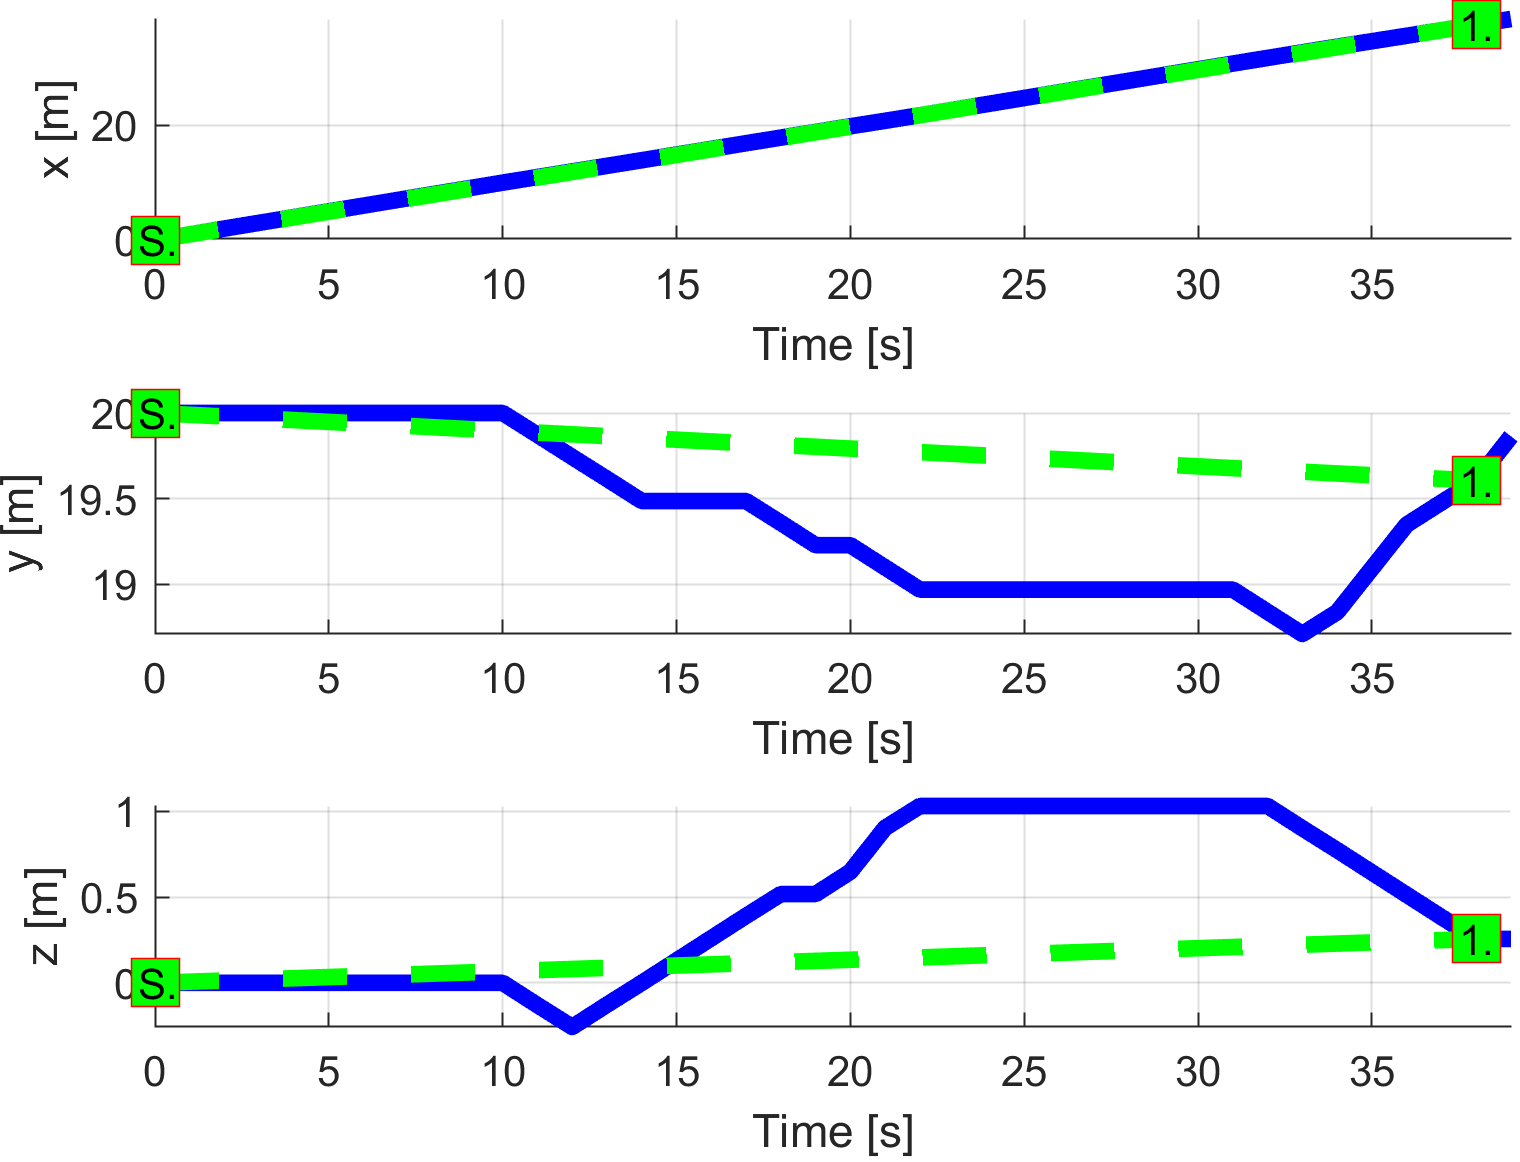
\includegraphics[width=0.9\linewidth]{\FIGDIR/NS037UtmEmergencyHeadOnUAV1PathFollowing}
        \caption{UAS 1.}
        \label{fig:emergencyHeadOnUAS1PathTracking}
    \end{subfigure}
    \begin{subfigure}{0.48\textwidth}
    	\centering
        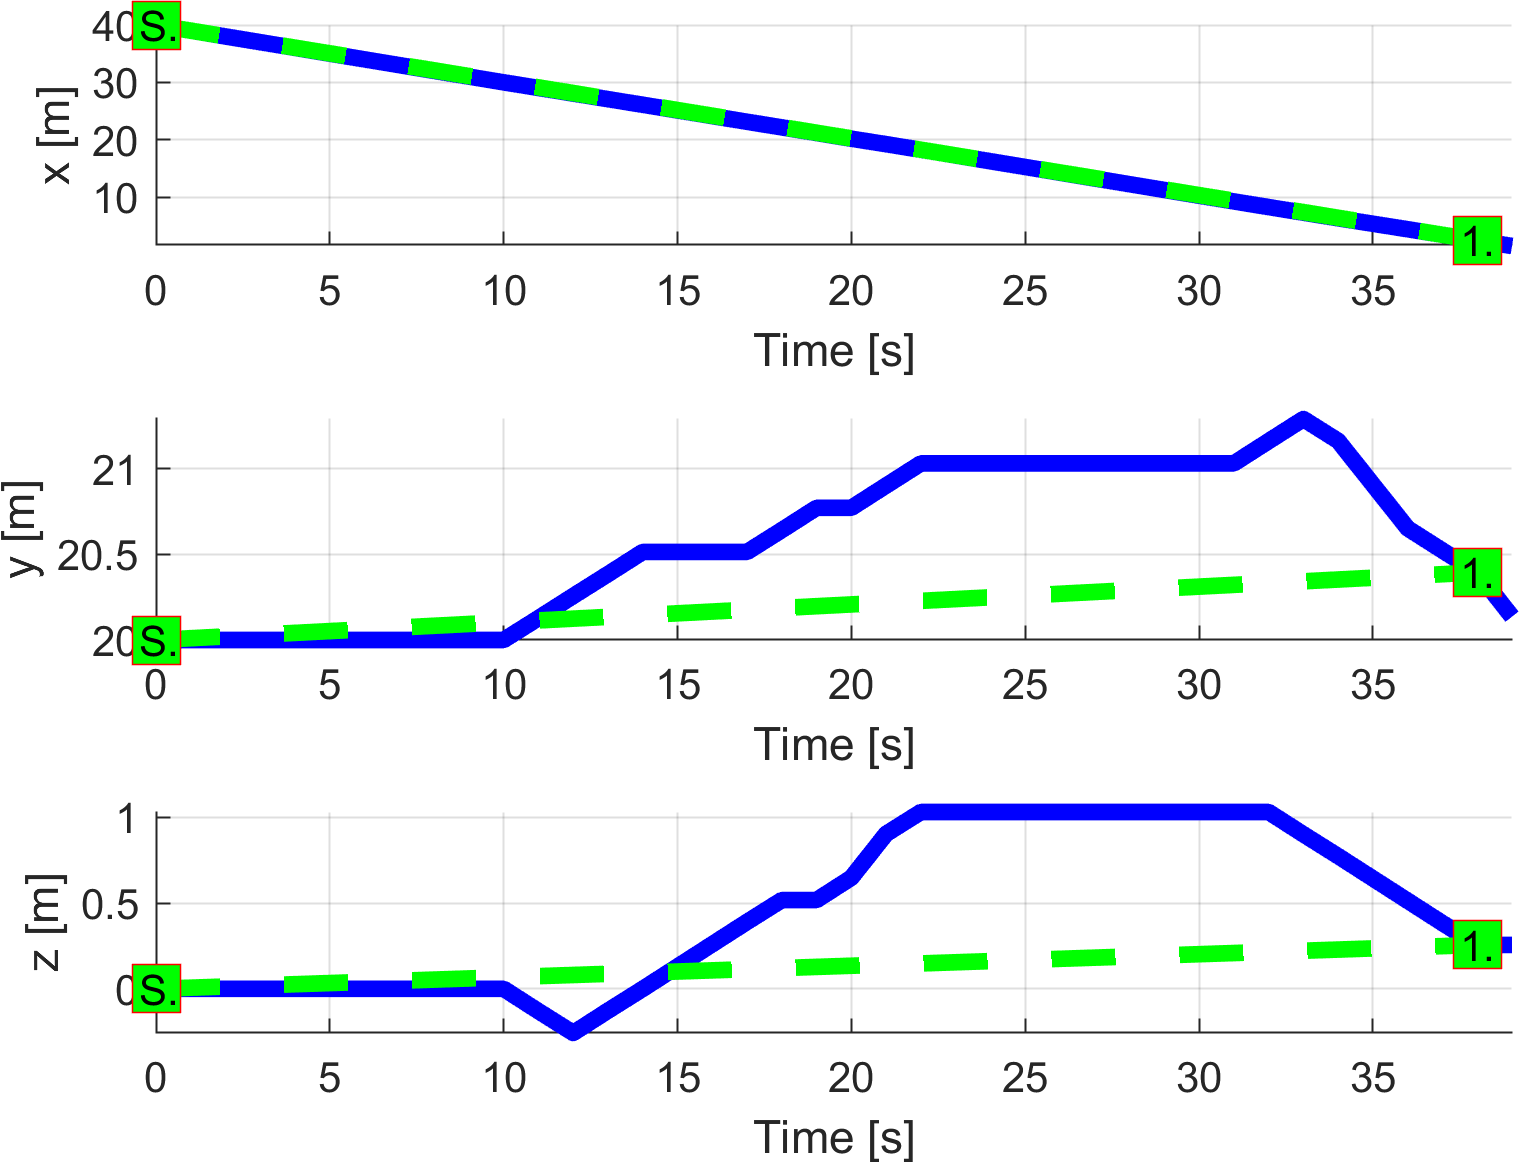
\includegraphics[width=0.9\linewidth]{\FIGDIR/NS038UtmEmergencyHeadOnUAV2PathFollowing} 
        \caption{UAS 2.}
        \label{fig:emergencyHeadOnUAS2PathTracking}
    \end{subfigure}
    \caption{\emph{Trajectory tracking} for \emph{Emergency head on} test case. }
    \label{fig:emergencyHeadOnTrajectoryTrackingPerformance}
\end{figure}


\paragraph{Path Following Deviations:} \emph{Deviations} (tab. \ref{tab:pathTrackingParametersForEmergencyHeadOn}) are in expected ranges considering the \emph{mission plans} (tab. \ref{tab:missionSetupEmergencyHeadOnScenario}) and \emph{separation safety margins} (tab. \ref{tab:aboidanceParametersForEmergencyHeadOnScenario}).


\begin{table}[H]
    \centering
    \begin{tabular}{c||c|c}
        \multirow{2}{*}{Param.} & UAS 1     & UAS 2\\\cline{2-3}
                        & $\mathscr{WP}_1$  & $\mathscr{WP}_1$\\\hline\hline
          $\max |x|$    & 0.05              & 0.06 \\\hline
          $\max |y|$    & 1.37              & 1.48 \\\hline
          $\max |z|$    & 1.03              & 1.05 \\\hline
          $\max dist.$  & 1.39              & 1.52 \\
    \end{tabular}
    \caption{Path tracking properties for \emph{Emergency head on} scenario.}
    \label{tab:pathTrackingParametersForEmergencyHeadOn}
\end{table}
    	\subsection{Emergency Mixed Head on with Converging}\label{s:testEmergencyMixed}

    \noindent\paragraph{Scenario:} \emph{Four UAS} are flying in an \emph{uncontrolled airspace} (altitude $\le$ 500 ft. Above the Ground Level) missions defined in (tab. \ref{tab:missionSetupEmergencyMixedScenario}). All UAS are in the \emph{Navigation mode} with active \emph{ADS-B In}, receiving \emph{position notifications} from each other. Cruising altitude is sufficient for \emph{horizontal separation} (50-100 ft. Above the Ground Level).
    
    
    \begin{table}[H]
        \centering
        \begin{tabular}{c||c|c||c}
            \multirow{2}{*}{UAS} &\multicolumn{2}{c||}{Position} & \multirow{2}{*}{$\mathscr{WP}_1$} \\\cline{2-3}
              & $[x,y,z]$           & $[\theta,\varpi,\psi]$           & \\\hline\hline
            1 & $[0,20,0]^T $       & $[0^\circ,0^\circ,0^\circ]^T$    & $[45,20,0]^T$\\\hline 
            2 & $[40,20,0]^T $       & $[0^\circ,0^\circ,180^\circ]^T$    & $[-5,20,0]^T$\\\hline 
            3 & $[20,0,0]^T $       & $[0^\circ,0^\circ,90^\circ]^T$    & $[20,45,0]^T$\\\hline 
            4 & $[20,40,0]^T $       & $[0^\circ,0^\circ,-90^\circ]^T$  & $[45,20,0]^T$\\ 
        \end{tabular}
        \caption{Mission setup for \emph{Emergency mixed} scenario.}
        \label{tab:missionSetupEmergencyMixedScenario}
    \end{table}
    
    \begin{note}
        \emph{Collision point} is expected at $\mathscr{C}=[20,20,0]^T$
    \end{note}
    
    \noindent \paragraph{Main Goal:} Show \emph{multiple non-cooperative intruders avoidance capability} in \emph{uncontrolled} airspace.
    
    \noindent \paragraph{Acceptance criteria:}
    \begin{enumerate}
        \item \emph{Proper avoidance mode invocation} - when an  \emph{intruder intersection model} impact the \emph{Avoidance Grid}, UAS system will switch to an \emph{Emergency avoidance mode}.
        
        \item\emph{Minimal safety margin distance} $\ge$ $0 m$.
        
        \item Each \emph{UAS} will reach own goal waypoint (tab. \ref{tab:missionSetupEmergencyMixedScenario}).
    \end{enumerate}
    
    
    \noindent\paragraph{Testing setup:} The \emph{standard test setup} for each UAS defined in (tab \ref{tab:testMovementOrientations}, \ref{tab:testUASBasicParameters}, \ref{tab:testNavigationGridBasic}, \ref{tab:testAvoidanceGridBasic}, \ref{tab:testUASColoring}) is used with following without parameter override.

    \emph{Intruder intersection} model has been chosen depending on UAS (tab. \ref{tab:aboidanceParametersForEmergencyMixedScenario}). Each UAS is equipped with \emph{ADS-B In/Out} sensor obtaining/distributing following information:
    \begin{enumerate}
        \item \emph{Position} - in operational section coordinate frame.
        \item \emph{Velocity} - vector representation in given coordinate frame.
        \item \emph{Class size} - class body radius based on UAS propulsion and size.
        \item \emph{Safety margin set} - set of safety margins for different collision cases.
    \end{enumerate}
    
    \emph{Avoidance parameters} for \emph{Emergency mixed scenario} are given in (tab. \ref{tab:aboidanceParametersForEmergencyMixedScenario}). Each UAS has different \emph{intruder model} and separation combination. Each UAS has same speed set to $1 m s^{-1}$. None of UAS has the \emph{Right of The Way}. 
    
    \emph{Safety margin} is considered as sum of both participants \emph{near miss margins}. In this case default safety margin is considered as $1.2$  $m$.
    
    \begin{table}[H]
        \centering
        \begin{tabular}{c||c|c|c||c|c||c}
            \multirow{2}{*}{UAS} & \multicolumn{3}{c||}{Parameters} & \multicolumn{2}{c||}{Margins} & \multirow{2}{*}{Separation}\\\cline{2-6}
                                 & velocity & intruder model & ROW        & body & safety                                        \\\hline\hline
            1                    & 1        & body + spread  & false            & 0.3         & 0.6           & horizontal       \\\hline
            2                    & 1        & body (timed)   & false            & 0.3         & 0.6           & vertical         \\\hline
            3                    & 1        & body (timed)   & false            & 0.3         & 0.6           & horizontal       \\\hline
            2                    & 1        & body + spread  & false            & 0.3         & 0.6           & vertical         \\
        \end{tabular}
        \caption{Avoidance parameters for  \emph{Emergency mixed} scenario.}
        \label{tab:aboidanceParametersForEmergencyMixedScenario}
    \end{table}
    
    \begin{note}
        Each \emph{UAS} use different intruder intersection models and primary \emph{separations} (defined in tab. \ref{tab:aboidanceParametersForEmergencyMixedScenario}).  UAS reactions are based on primary \emph{Separation} mode, intruders intersection models this is reflected on major axial deviations in (fig. \ref{fig:testCaseEmergencyMixedTrajectoryTracking}) and summarized in \emph{path tracking} deviation (tab. \ref{tab:pathTrackingParametersForEmergencyMixed}).
    \end{note}
    
    \noindent\paragraph{Simulation Run:} Notable moments from the simulation run (fig. \ref{fig:testCaseEmergencyMixed}) are following:
    
    \begin{enumerate}
        \item \emph{Situation detection} (fig. \ref{fig:emergencyMultipleSituationDetection}) - UAS 1 (blue) is detecting UAS 2 (cyan), UAS 3 (green), and UAS 4 (black) as possible intruders. There are multiple converging and head on approaches depending on mutual positions (UAS and \emph{angle of approach}). There exist at least one \emph{converging case} where each UAS has \emph{Right of the way}. Each UAS creates intruder intersection models depending on the intruder configuration (tab. \ref{tab:aboidanceParametersForEmergencyMixedScenario}). Each UAS enters into the \emph{Emergency avoidance mode} independently, when at least one trajectory is constrained in the \emph{avoidance grid}. 
        
        \item \emph{Before near miss} (fig. \ref{fig:emergencyMultipleBeforeNearMiss}) - all \emph{UAS} are in \emph{emergency avoidance mode}, using various \emph{separation modes} and \emph{intruder intersection models}. Each UAS is performing its own avoidance maneuver, constantly checking other intruders. If same separation and same intruder model was used, there will be virtual roundabout.
            
        \item \emph{After near miss} (fig. \ref{fig:emergencyMultipleAfterNearMiss}) - all \emph{UAS} avoided each other which is covered in \emph{safety margin performance} (fig. \ref{fig:testCaseMultipleAvoidancePerformance}) and (tab. \ref{tab:testCaseEmergencyMixedSafetyMarginDistances}).
        
        \item \emph{Situation resolution} (fig. \ref{fig:emergencyMultipleSituationReslution}) - all \emph{UAS}
        returns to \emph{Navigation mode} correcting \emph{altitude} first and continuing to assigned waypoints.
    \end{enumerate}
    
    \begin{figure}[H]
        \centering
        \begin{subfigure}{0.48\textwidth}
        	\centering
            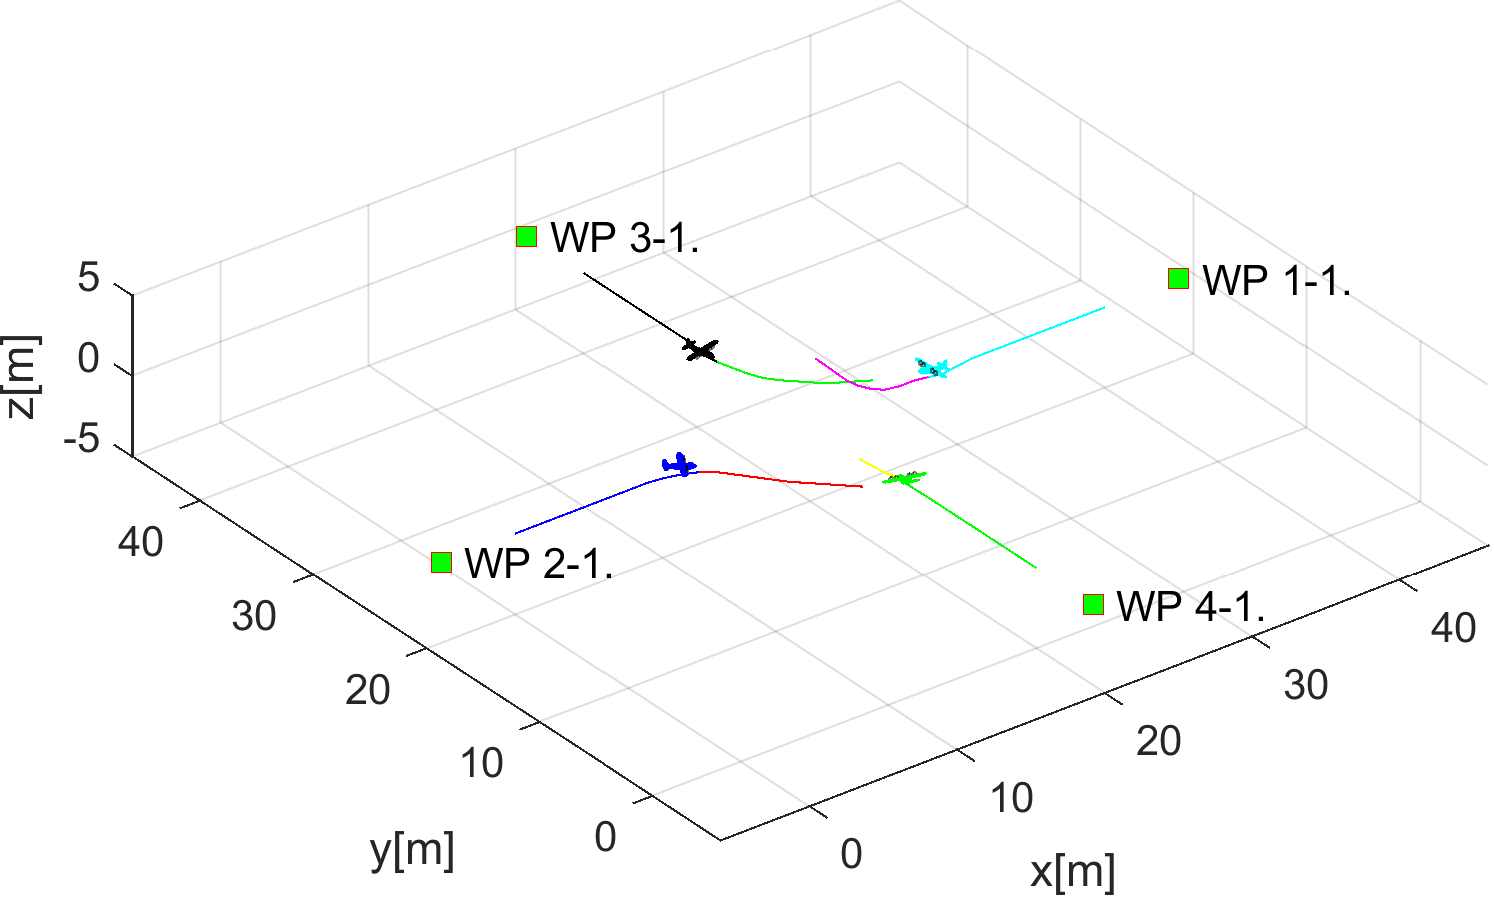
\includegraphics[width=0.9\linewidth]{\FIGDIR/NS039UtmEmergencyHeadOnMultiple00012}
            \caption{Situation detection.}
            \label{fig:emergencyMultipleSituationDetection}
        \end{subfigure}
        \begin{subfigure}{0.48\textwidth}
        	\centering
            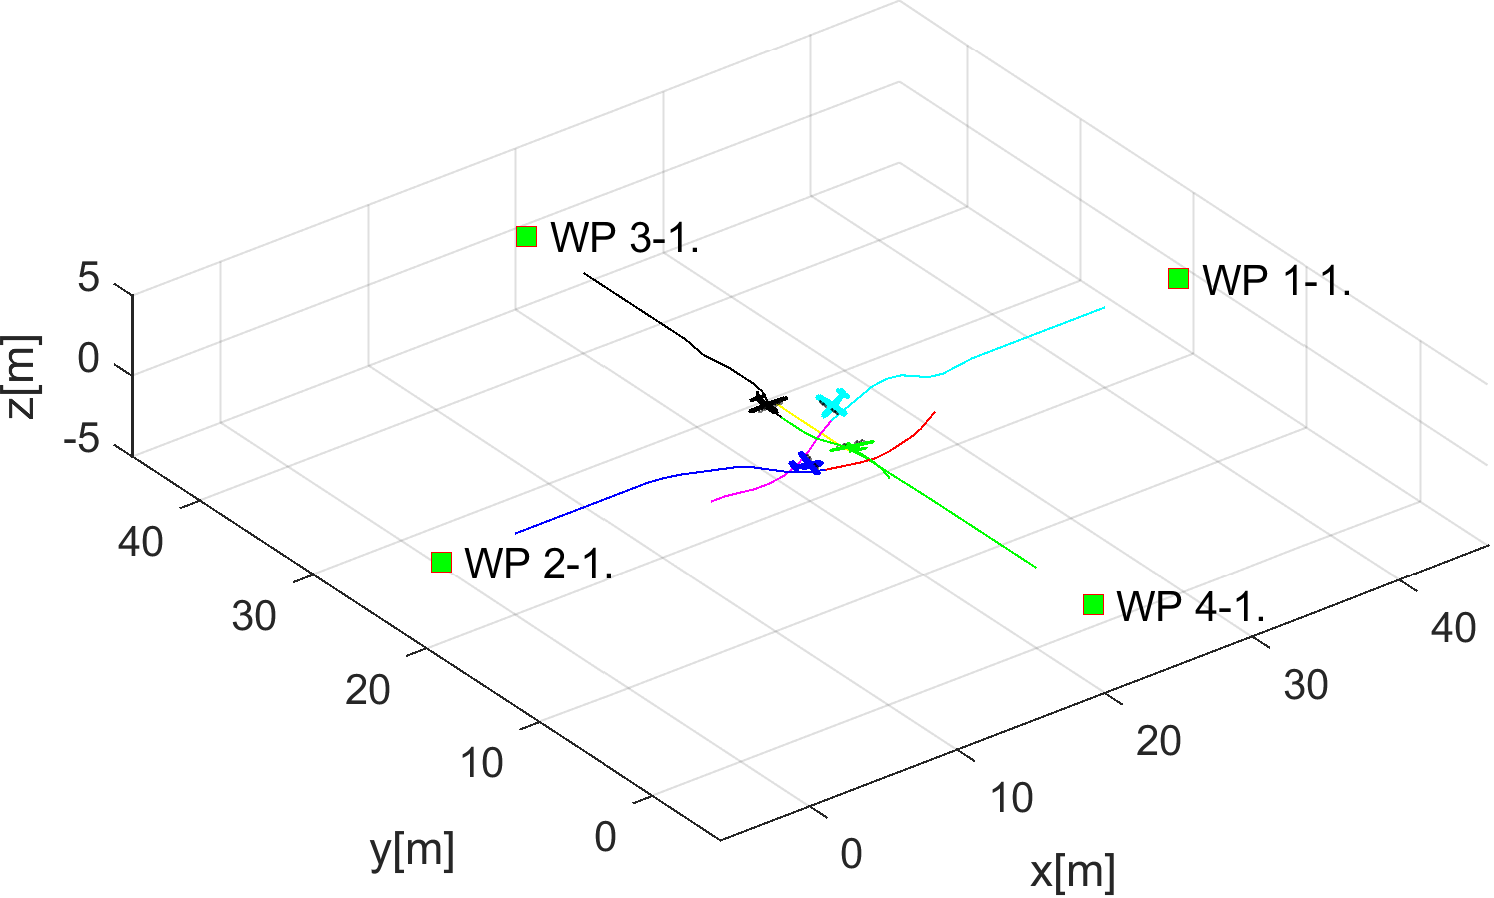
\includegraphics[width=0.9\linewidth]{\FIGDIR/NS040UtmEmergencyHeadOnMultiple00019} 
            \caption{Before near miss.}
            \label{fig:emergencyMultipleBeforeNearMiss}
        \end{subfigure}
        \\
        \begin{subfigure}{0.48\textwidth}
        	\centering
            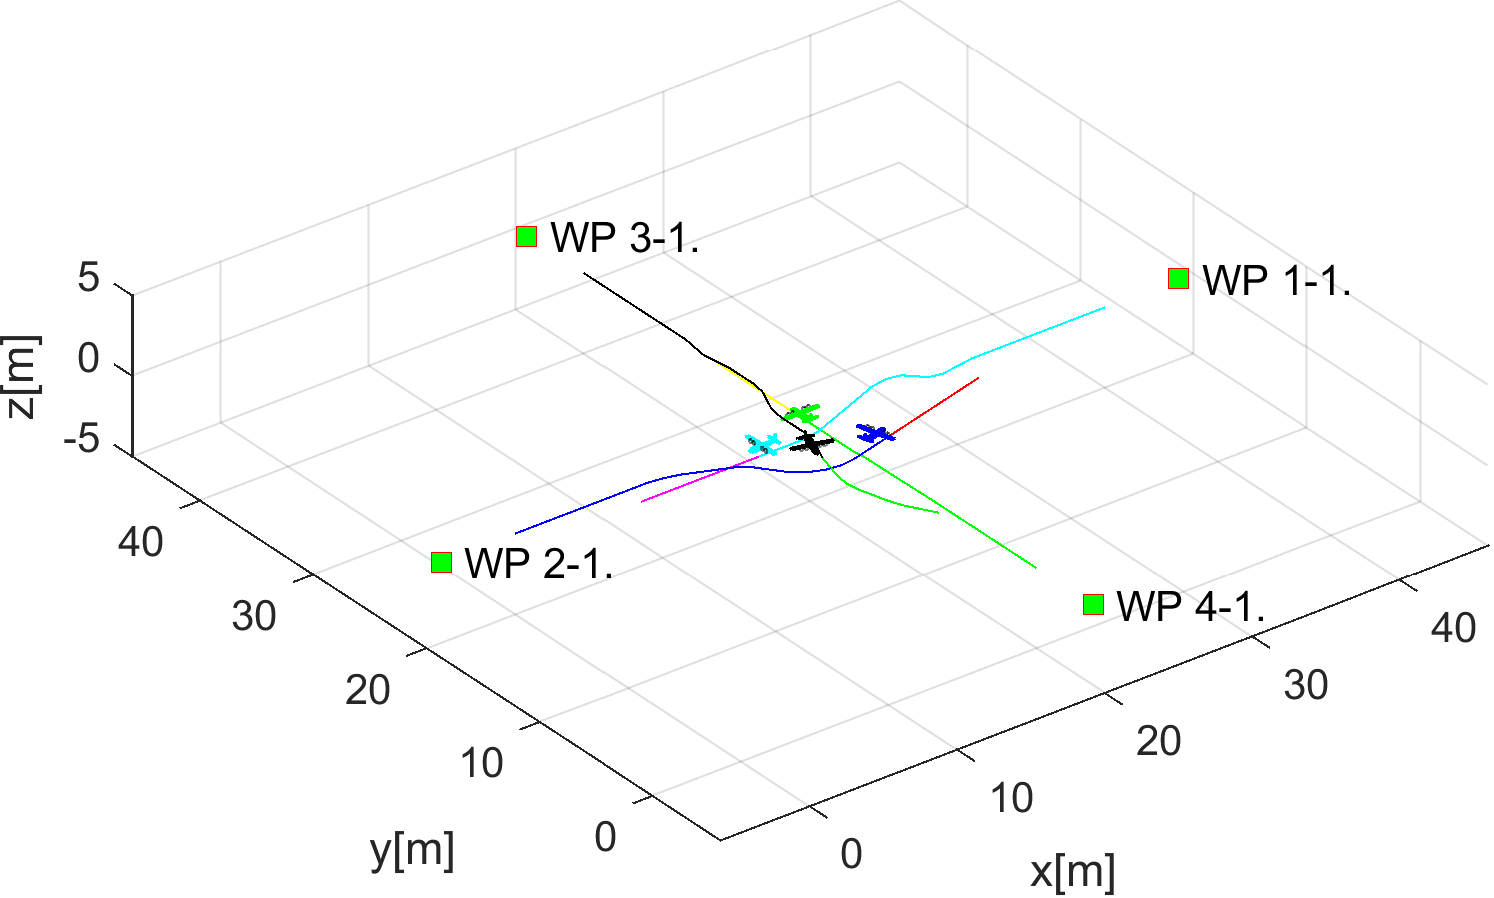
\includegraphics[width=0.9\linewidth]{\FIGDIR/NS041UtmEmergencyHeadOnMultiple00024} 
            \caption{After near miss.}
            \label{fig:emergencyMultipleAfterNearMiss}
        \end{subfigure}
        \begin{subfigure}{0.48\textwidth}
        	\centering
            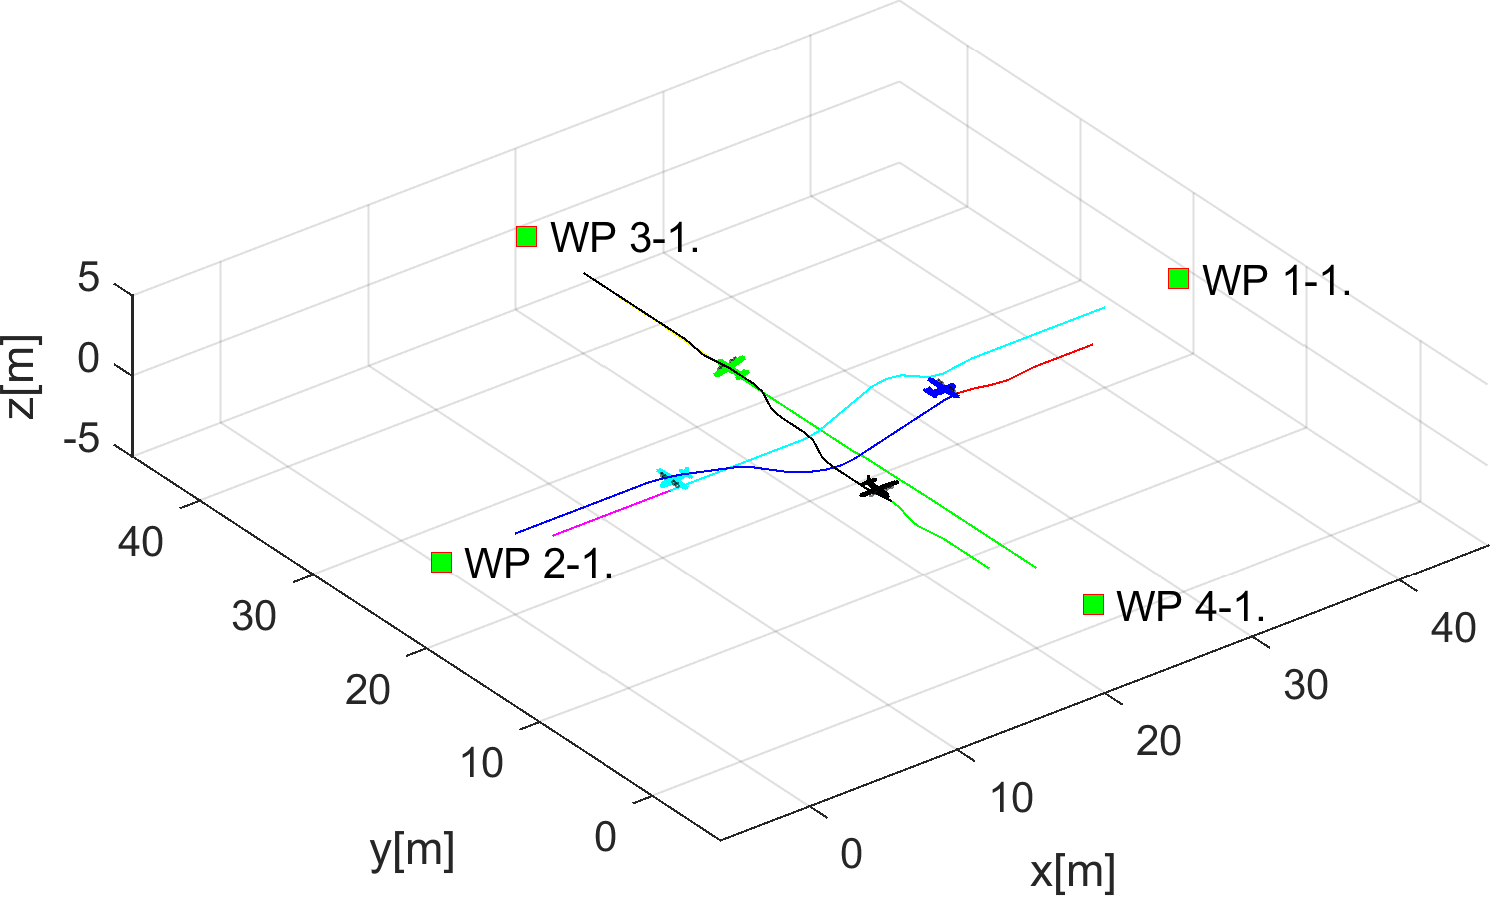
\includegraphics[width=0.9\linewidth]{\FIGDIR/NS042UtmEmergencyHeadOnMultiple00030} 
            \caption{Situation resolution.}
            \label{fig:emergencyMultipleSituationReslution}
        \end{subfigure}
        \caption{Test scenario for \emph{Emergency mixed} situation with \emph{self-separation mode}.}
        \label{fig:testCaseEmergencyMixed}
    \end{figure}
    
    \paragraph{Distance to Safety Margin Evolution:} There is need to compare mutual distance between each UAS. The graph (fig. \ref{fig:testCaseMultipleAvoidancePerformance}) shows six figures for each \emph{UAS systems} mutual distance (blue line) in this scenario. The \emph{Safety Margin} (red line) ($1.2$ $m$) was not breached for any pair (case). 
    
    The \emph{Proper avoidance invocation} is shown when UAS systems are getting closer to each other and then they start separation phase (Emergency avoidance mode).
            
    \begin{figure}[H]
        \centering
        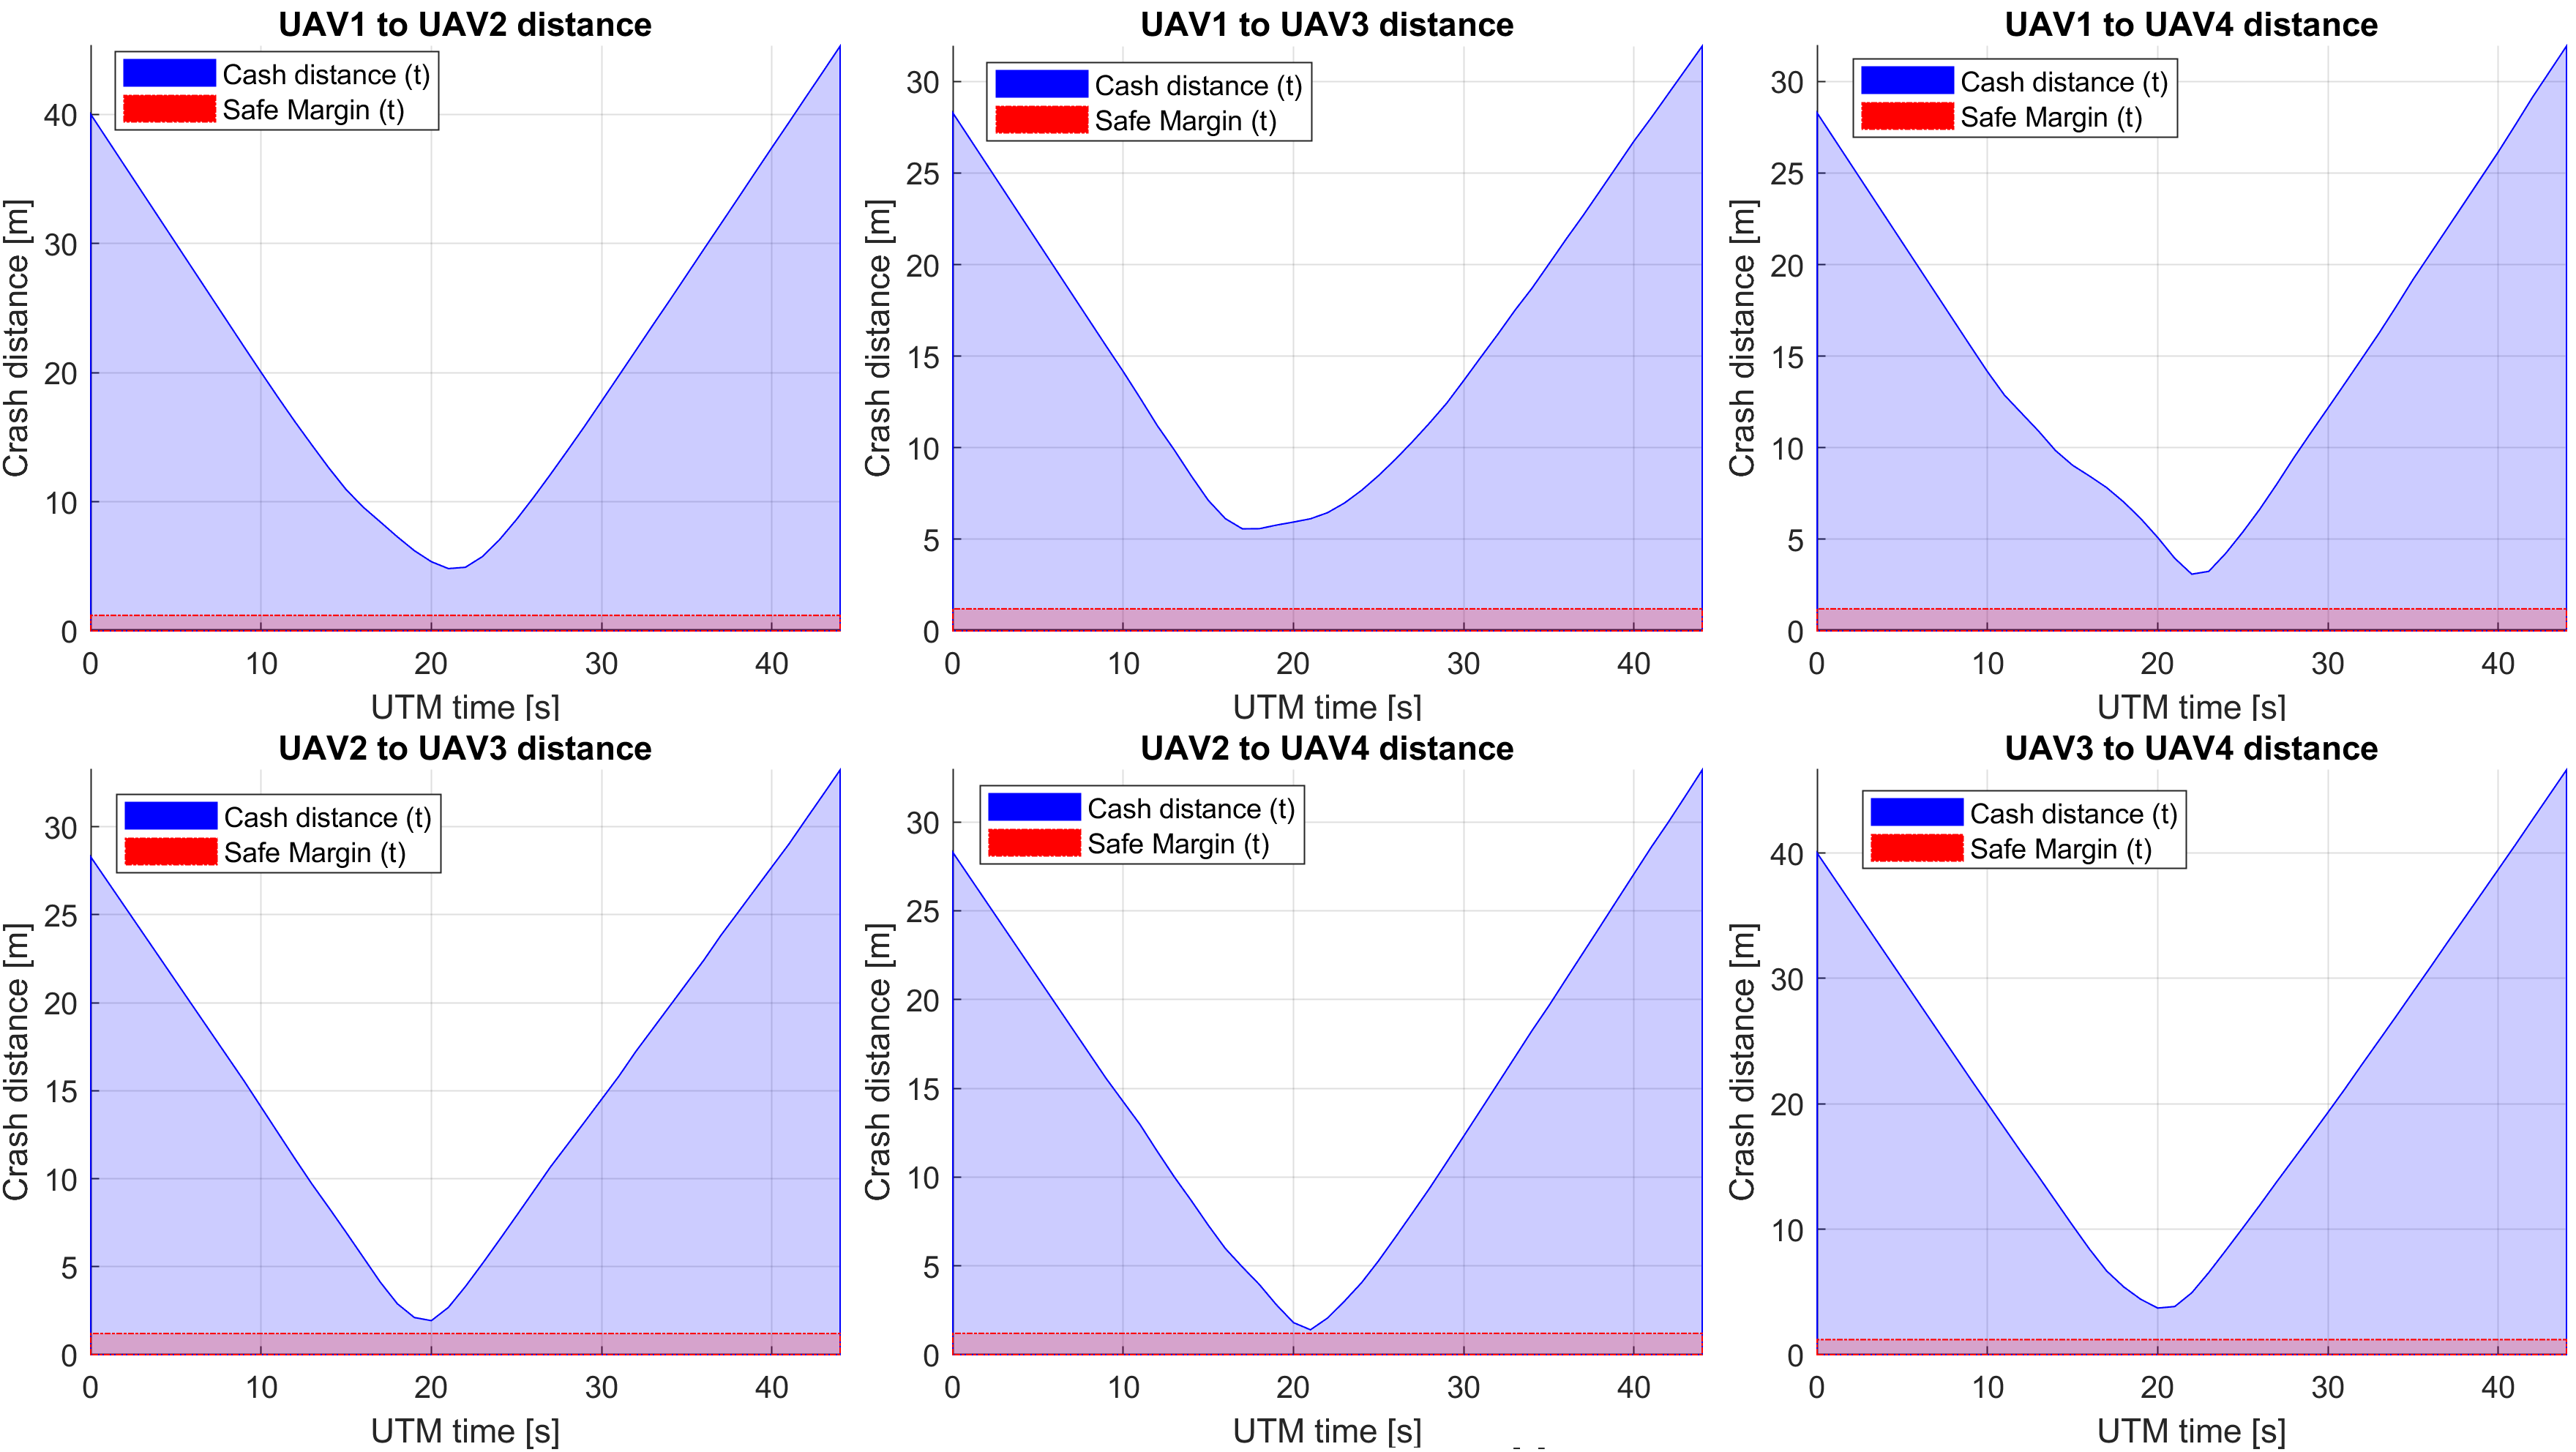
\includegraphics[width=0.9\linewidth]{\FIGDIR/NS043UtmEmergencyHeadOnMultiplePerformance} 
        \caption{Distance to safety margin evolution for \emph{emergency mixed scenario}.}
        \label{fig:testCaseMultipleAvoidancePerformance}
    \end{figure}
    
    \paragraph{Distance to Safety Margin Peaks:} Minimal and Maximal mutual distance to safety margin is summarized in (tab. \ref{tab:testCaseEmergencyMixedSafetyMarginDistances}). There is no detected breach for any combination. 
    
    The \emph{closest to collision} is UAS pair $2-4$ with mutual safety margin only $0.2019$ $m$. On the other side is UAS pair $1-3$ with mutual safety margin $4.3721$ $m$. 
    
    The \emph{minimal distance to safety margin}  $\ge$ 0 which means that the \emph{safety condition} is fulfilled. 
    
    \begin{table}[H]
        \centering
        \begin{tabular}{c||c|c|c}
            \multirow{2}{*}{UAS:} & \multicolumn{3}{c}{Distance to Safety Margin} \\ \cline{2-4} 
                      & min          & max         & breach         \\ \hline\hline
                1-2   & 3.6231       & 44.0831     & false          \\ \hline
                1-3   & 4.3721       & 30.7300     & false          \\ \hline
                1-4   & 1.8959       & 30.7331     & false          \\ \hline
                2-3   & 0.7331       & 32.0266     & false          \\ \hline
                2-4   & 0.2019       & 31.7282     & false          \\ \hline
                3-4   & 2.5171       & 45.4257     & false          \\ 
        \end{tabular}
        \caption{Distance to safety margin peaks for \emph{emergency mixed scenario}.}
        \label{tab:testCaseEmergencyMixedSafetyMarginDistances}
    \end{table}
    
    \noindent\paragraph{Path Tracking Performance:} All waypoints (Green numbered squares) for all UAS have been reached (fig. \ref{fig:testCaseEmergencyMixedTrajectoryTracking}). \emph{Reference trajectories} (green dashed line) have been tracked by \emph{UAS real path} (blue solid line) almost all time. 
    
    Following observations can be made from \emph{path tracking} (fig. \ref{fig:testCaseEmergencyMixedTrajectoryTracking}) and \emph{preferred separations} (tab. \ref{tab:aboidanceParametersForEmergencyMixedScenario}):
    
    \begin{enumerate}
        \item UAS 1 (fig. \ref{fig:emergencyMixedPathTrackingUAS1}) is using \emph{horizontal separation} (y axis right) having \emph{preferred horizontal separation}.
        
        \item UAS 2 (fig. \ref{fig:emergencyMixedPathTrackingUAS2}) is using vertical separation (z axis up-down), having preferred vertical separation.
        
        \item UAS 3 (fig. \ref{fig:emergencyMixedPathTrackingUAS3}) is using horizontal/vertical separation (x right, z down), having preferred horizontal separation.  This UAS has used other than preferred separation type.
        
        \item UAS 4 (fig. \ref{fig:emergencyMixedPathTrackingUAS4}) is using horizontal separation (x-axis right/left), having preferred vertical separation. This UAS has used opposite separation type, than preferred.
    \end{enumerate}
    
    
    \begin{figure}[H]
        \centering
        \begin{subfigure}{0.48\textwidth}
        	\centering
            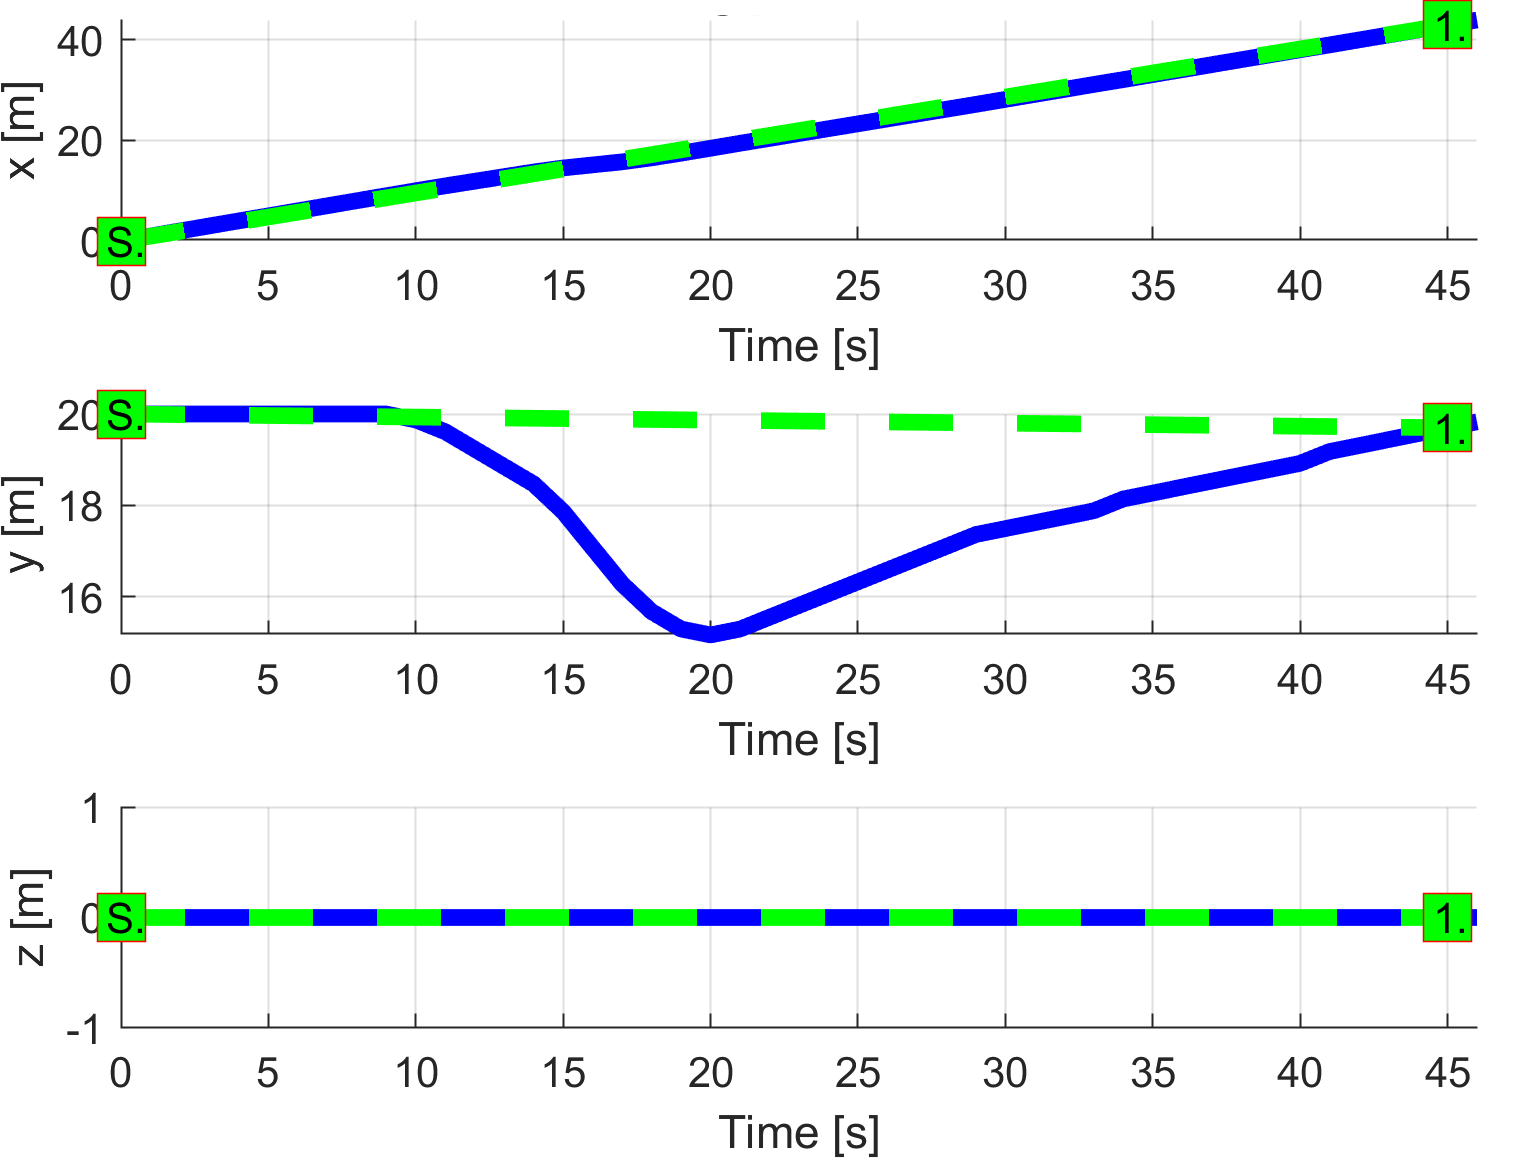
\includegraphics[width=0.9\linewidth]{\FIGDIR/NS044UtmEmergencyHeadOnMultipleUAV1PathFollowing}
            \caption{UAS 1.}
            \label{fig:emergencyMixedPathTrackingUAS1}
        \end{subfigure}
        \begin{subfigure}{0.48\textwidth}
        	\centering
            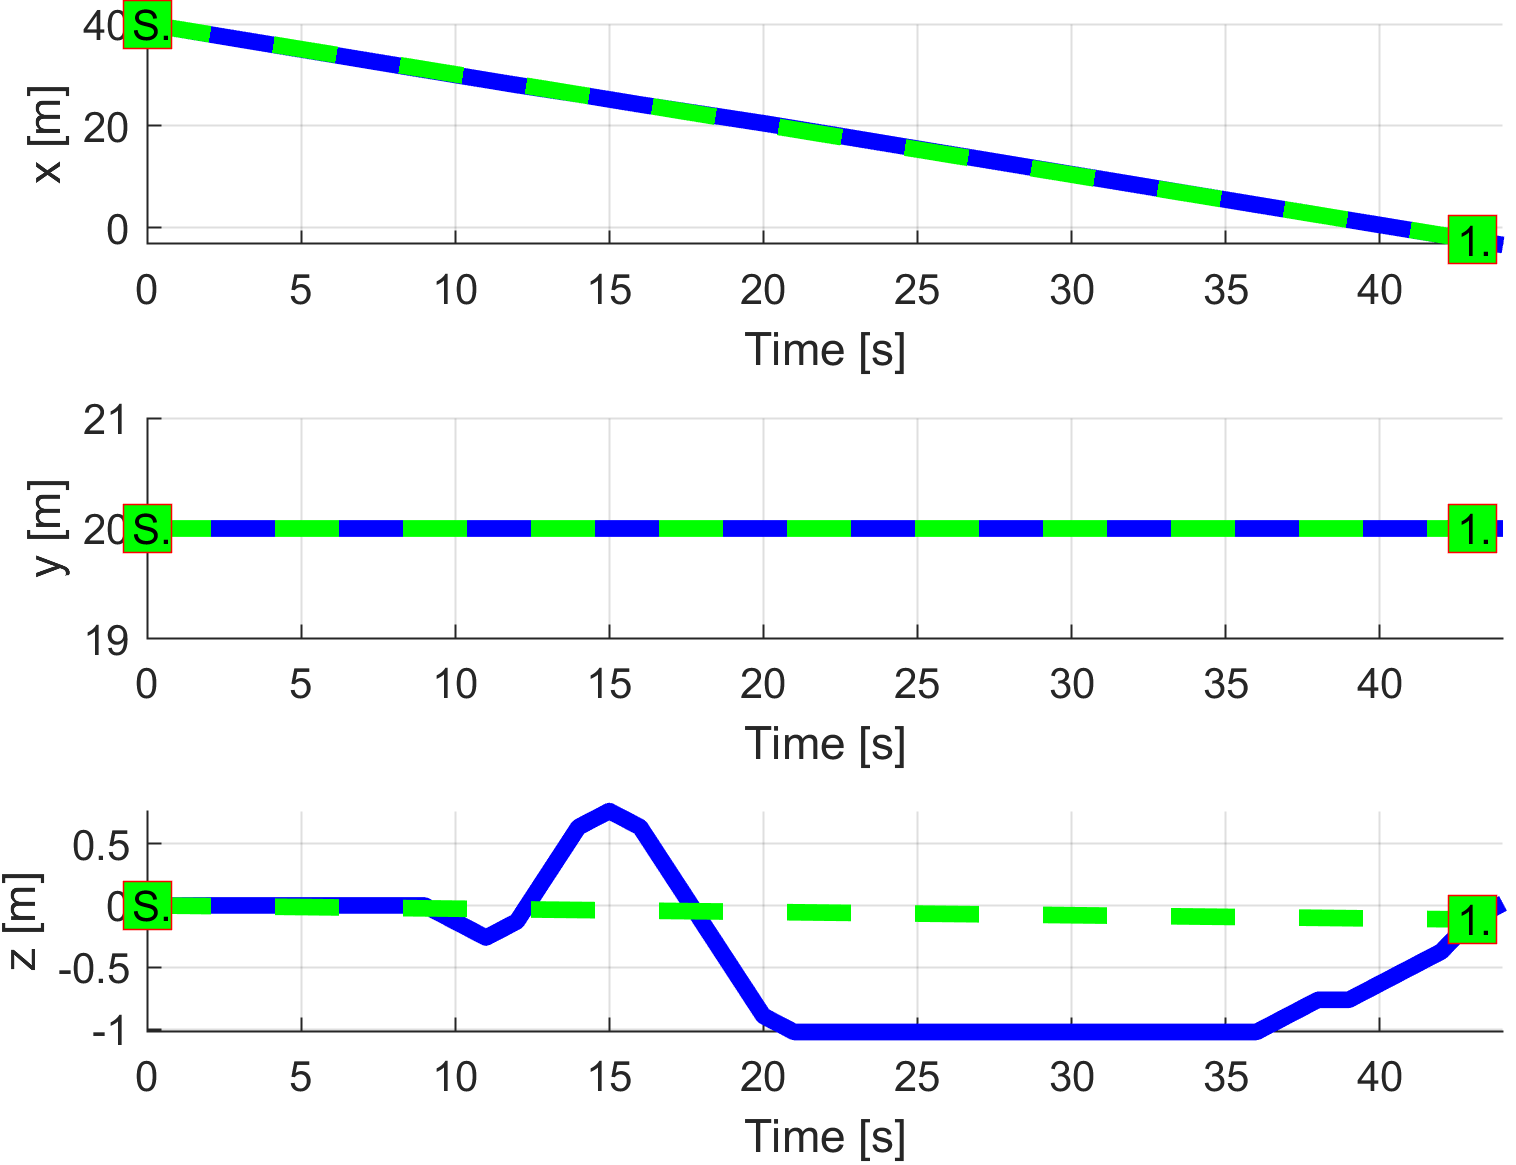
\includegraphics[width=0.9\linewidth]{\FIGDIR/NS045UtmEmergencyHeadOnMultipleUAV2PathFollowing} 
            \caption{UAS 2.}
            \label{fig:emergencyMixedPathTrackingUAS2}
        \end{subfigure}
        \\
        \begin{subfigure}{0.48\textwidth}
        	\centering
            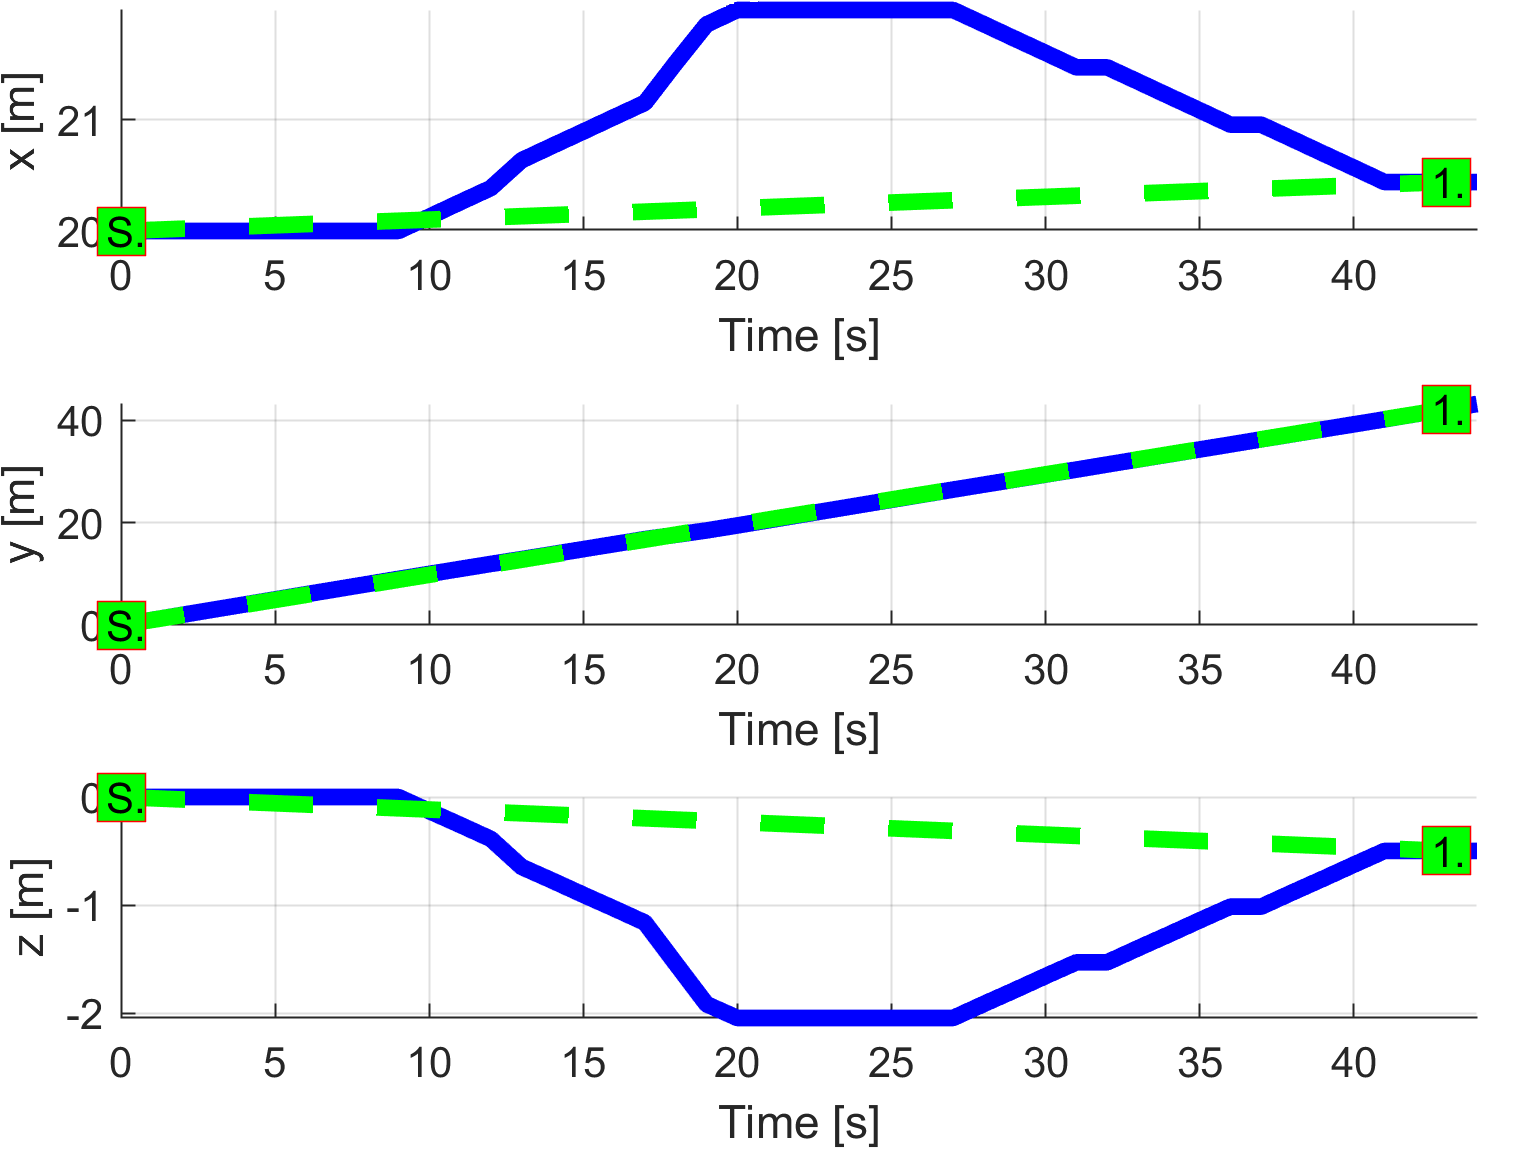
\includegraphics[width=0.9\linewidth]{\FIGDIR/NS046UtmEmergencyHeadOnMultipleUAV3PathFollowing} 
            \caption{UAS 3.}
            \label{fig:emergencyMixedPathTrackingUAS4}
        \end{subfigure}
        \begin{subfigure}{0.48\textwidth}
        	\centering
            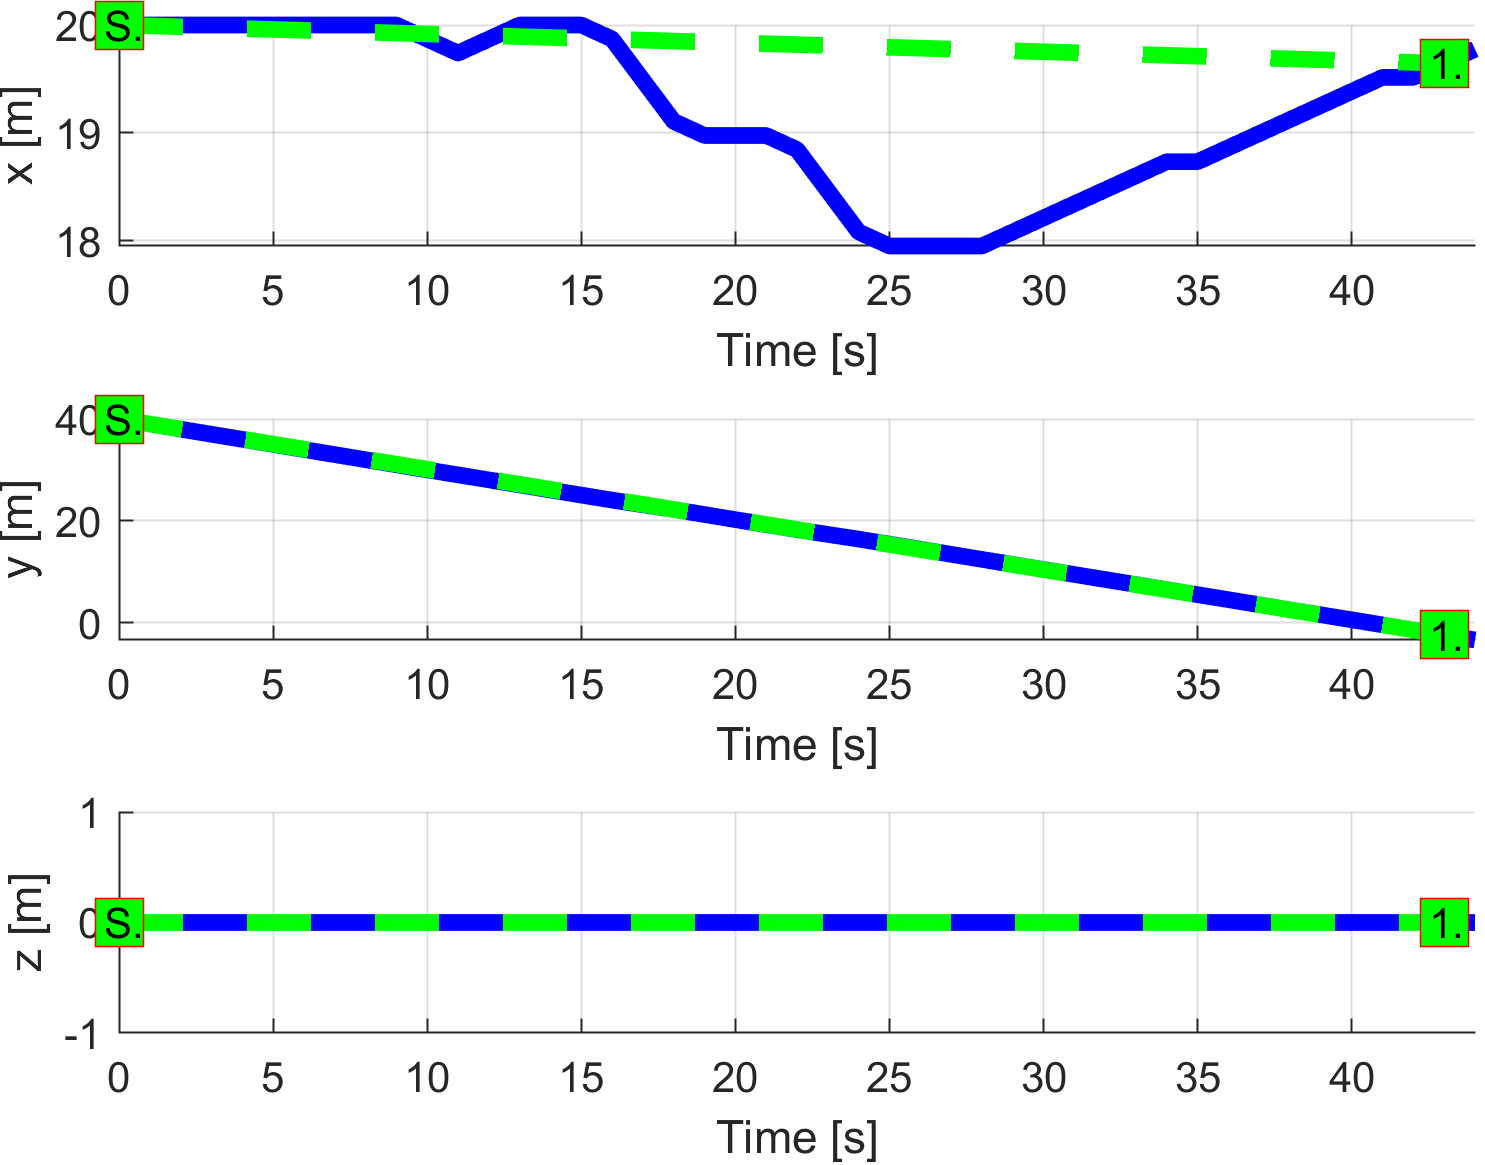
\includegraphics[width=0.9\linewidth]{\FIGDIR/NS047UtmEmergencyHeadOnMultipleUAV4PathFollowing} 
            \caption{UAS 4.}
            \label{fig:emergencyMixedPathTrackingUAS3}
        \end{subfigure}
        \caption{Trajectory tracking for \emph{Emergency mixed} situation test case.}
        \label{fig:testCaseEmergencyMixedTrajectoryTracking}
    \end{figure}
    
    \noindent\paragraph{Path Tracking Deviations:} \emph{Deviations} (tab. \ref{tab:pathTrackingParametersForEmergencyMixed}) are in expected ranges considering the \emph{mission plans} (tab. \ref{tab:missionSetupEmergencyMixedScenario}) and \emph{separation safety margins} (tab. \ref{tab:aboidanceParametersForEmergencyMixedScenario}).
    
    \begin{table}[H]
        \centering
        \begin{tabular}{c||c|c|c|c}
            \multirow{2}{*}{Param.} & UAS 1     & UAS 2             & UAS 3             & UAS 4 \\\cline{2-5}
                            & $\mathscr{WP}_1$  & $\mathscr{WP}_1$  & $\mathscr{WP}_1$  & $\mathscr{WP}_1$ \\\hline\hline
              $\max |x|$    & 0                 & 0                 & 1.98              & 2.05\\\hline
              $\max |y|$    & 4.84              & 0                 & 0                 & 0\\\hline
              $\max |z|$    & 0                 & 1.23              & 2.43              & 0\\\hline
              $\max dist.$  & 4.84              & 1.23              & 3.45              & 2.05\\
        \end{tabular}
        \caption{Path tracking properties for \emph{Emergency mixed} scenario.}
        \label{tab:pathTrackingParametersForEmergencyMixed}
    \end{table}    



    
    %Observations moved to Conclusion - no longer in use
    %\section{(W) Simulation Observations Summary}\label{sec:SimulationObservationsSummary}
    \noindent Use summary of this section in Conclusion and future work on specific 

\subsection{(W) Static Obstacles Avoidance}\label{sec:staticObstacleAvoidanceSummary}
    \noindent TODO: main points of building, slalom, maze scenarios - link artifacts and performance criteria

\subsection{(W) Constraints Avoidance}\label{sec:constraintAvoidanceSummary}
    \noindent TODO constraints main point, main loop processing, breach chance ? etc...
    
\subsection{(W) Unsupervised Intruder Avoidance}\label{sec:unsupervisedIntruderAvoidance}
    \noindent TODO emergency intruder avoidance emphasis navigation, Emergency avoidance contribution main points

\subsection{(W) Supervised (UTM) Intruder Avoidance}\label{sec:supervisedIntruderAvoidance}
    \noindent TODO UTM contribution main points
    
 

%% This adds a line for the Bibliography in the Table of Contents.
\addcontentsline{toc}{chapter}{Bibliography}
%% *** Set the bibliography style. ***
%% (change according to your preference/requirements)
%\bibliographystyle{plain}
%% *** Set the bibliography file. ***
%% ("thesis.bib" by default; change as needed)
\bibliography{thesis}

%% *** NOTE ***
%% If you don't use bibliography files, comment out the previous line
%% and use \begin{thebibliography}...\end{thebibliography}.  (In that
%% case, you should probably put the bibliography in a separate file and
%% `\include' or `\input' it here).

\end{document}
